\documentclass[a4paper, 12pt, twoside]{report}  % Use report class for thesis
\usepackage{uarial}
\usepackage{graphicx}   % For inserting the university logo
\usepackage{setspace}   % For line spacing
\usepackage{titlesec}   % For title formatting
\usepackage[left=38mm, right=25mm, top=25mm, bottom=25mm]{geometry}
\usepackage{indentfirst}
\usepackage{afterpage}
\usepackage{titlesec}
\usepackage{caption} % For figures' caption
\usepackage{url} % For adding url, mainly in references
\usepackage{pdfpages} % To include PDFs
\usepackage{amsmath} % For pseudo codes
\usepackage{algorithm} % For pseudo codes
\usepackage{algpseudocode} % For pseudo codes
\algrenewcommand\algorithmicrequire{\textbf{Input:}} % For pseudo codes
\algrenewcommand\algorithmicensure{\textbf{Output:}} % For pseudo codes

\onehalfspacing  % Set line spacing to 1.5

\begin{document}

% Title Page
\begin{titlepage}
    \newgeometry{left=38mm, right=30mm, top=30mm, bottom=30mm}

    \begin{center}
        
\includegraphics{Images/UNIMI.png} \\
        {\textit{Master’s Degree in Data Science for Economics}} \\[2cm]

        {\LARGE \textbf{Enhancing Needs-Based Segmentation:}} \\
        {\Large \textbf{\textit{Using Text Data Mining Framework for Attribute Discovery and Validation.}}} \\
        {\Large \textbf{\textit{An application in the field of Destination Branding.}}} \\[2cm]
    \end{center}

    \begin{flushleft}
        \textbf{Supervisor:} Prof. Massimo ALIBERTI \\
        \textbf{Co-Supervisor:} Prof. Stefano MONTANELLI  
    \end{flushleft}

    \vspace{2cm}

    \begin{flushright}
        \textbf{Thesis by:} \\ 
        \textbf{Franco Reinaldo BONIFACINI} \\ 
        Matr. 41540A
    \end{flushright}

    \vfill

    \begin{center}
        \textbf{Academic Year 2024/2025}
    \end{center}

    \restoregeometry % Restore original margins after titlepage
\end{titlepage}

\thispagestyle{empty}
\null
\cleardoublepage  % Ensures that the new section starts in an odd page.

\pagenumbering{roman}
\setcounter{page}{1}

\chapter*{Acknowledgments}
\addcontentsline{toc}{chapter}{Acknowledgments}

To my grandmother Chiche, who remains as present as ever. For her unconditional love, for always waiting for me with a smile, and for supporting me every step of the way, even from afar. Today she guides me from heaven, and her strength walks with me every day.

To Delfina, my wife, for being the person who always supports me and with whom I embarked on this beautiful adventure in a new continent. If it hadn’t been for her, I might never have dared to take this step.

To my family, especially my parents, because I know that this decision distanced us physically and was difficult for them, yet they have always supported me.

To Massimo and Giorgia, for guiding me through this final step of the master’s program, and for introducing me to the wonderful city of Ascoli Piceno.

To my friends from Argentina, and especially to all the friends I made during this beautiful experience here in Italy, who helped me grow personally, introduced me to new cultures and ways of life I never imagined I'd discover, and who stood by my side during the most difficult moments, encouraging me to never give up.

To myself, because despite my fear of flying, I had the courage to get on the plane and embark on this incredible journey. And, above all, for the perseverance to keep moving forward despite the obstacles along the way.

And finally, to this beautiful country where my bisnonno was from, which welcomed me and allowed me to have one of the greatest experiences of my life. I came as an Argentinian and now I am an ``Argentano," proud to have reconnected with my roots.

\begin{center}
    \rule{0.5\textwidth}{0.4pt} % Línea divisoria
\end{center}

A mi abuela Chiche, que sigue tan presente como siempre. Por su amor incondicional, por esperarme siempre con una sonrisa, y por apoyarme en cada paso, incluso en la distancia. Hoy me guía desde el cielo, y su fuerza me acompaña cada día.

A Delfina, mi esposa, por ser la persona que siempre me aguanta y con quien emprendí esta hermosa aventura en un nuevo continente. Si no hubiese sido por ella, quizá nunca me habría animado a dar este paso.

A mi familia, principalmente a mis padres, porque sé que esta decisión nos alejó físicamente y les costó, pero aun así siempre me apoyaron a la distancia.

A Massimo y Giorgia, por haberme acompañado en este último escalón del máster, y por haberme presentado a la hermosa ciudad que es Ascoli Piceno.

A mis amigos de Argentina, y principalmente todos los amigos que me hice en esta hermosa experiencia acá en Italia, quienes me hicieron crecer personalmente, me acercaron a nuevas culturas y formas de vivir que jamás imaginé conocer, y que en los momentos más difíciles estuvieron a mi lado, impulsándome a nunca bajar los brazos.

A mí mismo, porque más allá del miedo a volar, tuve el coraje de subirme al avión y emprender esta hermosa aventura. Y, sobre todo, por la perseverancia de seguir adelante a pesar de los obstáculos en el camino.

Y a este hermoso país del que era mi bisnonno y que me recibió para vivir una de las mejores experiencias de mi vida. Vine como argentino y ahora soy un ``argentano", orgulloso de haber vuelto a mis raíces.

\begin{flushright}
    \textbf{Franco Reinaldo Bonifacini}
\end{flushright}

\cleardoublepage

\tableofcontents

\newpage

\listoffigures

\newpage
\pagenumbering{arabic}

\begin{abstract}

    Tourism plays a fundamental role in the economic development of many Italian cities, including Ascoli Piceno, a destination with significant untapped potential. Despite its rich cultural, historical, and gastronomic heritage, the city has yet to establish itself as a highly competitive tourist destination compared to other Italian locations.

    This project analyzes tourism data from various Italian cities to identify key trends in visitor segmentation, pricing models, and market positioning. To address this challenge, this study seeks to answer the following research question: "What is the optimal combination of pricing, positioning, and promotional strategies for Ascoli Piceno to increase tourism competitiveness?". By combining secondary data analysis with primary research through surveys, the project provides insights into tourist preferences, spending behavior, and the effectiveness of different promotional strategies. Additionally, financial factors—including cost structures, potential partnerships, and the role of influencer marketing—are examined to understand their impact on tourism promotion.
        
    Using clustering techniques and strategic pricing models, the research proposes optimized tourism packages tailored to different market segments. The findings aim to offer evidence-based recommendations for Ascoli Piceno to improve its tourism appeal, increase visitor numbers, and strengthen its overall economic sustainability. Further research could explore the long-term effects of these strategies and identify additional factors that influence the competitiveness of tourist destinations.
\end{abstract}

\chapter{Introduction}

\indent This chapter introduces the context and motivation behind this thesis, which focuses on developing an efficient methodological framework for analyzing tourist behavior. It begins with an overview of the tourism sector, emphasizing its economic importance and the structural changes brought by the Covid-19 pandemic. The discussion then introduces Ascoli Piceno as a reference case. The chapter continues by outlining the previous project that served as the starting point for this research, identifying its main limitations and lessons learned. Finally, it reviews the current methodological approaches used in tourism analysis, highlighting the theoretical and practical gaps that motivate the development of a more integrated and adaptive analytical method.

\section{Touristic Context}

\indent Tourism is recognized as one of the most important economic sectors in the world. In 2019, it represented a significant share of the global economy, accounting for 7\% of global trade. However, despite its importance, tourism was also among the sectors most severely impacted by the Covid-19 pandemic, which affected not only global economies but also livelihoods, public services, and development opportunities in countries across all continents \cite{unwtocovid}. Now, four years after the onset of the pandemic, the sector has shown strong signs of recovery. International tourist arrivals have returned to 99\% of 2019 levels, signaling that tourism has bounced back from what is considered the worst crisis in its history \cite{unwtoppt}. As shown in Figure~\ref{fig:global_results}, in addition to the rebound in arrivals, there has also been a notable rise in international tourism revenues, reaching USD 1.7 trillion in 2024 \cite{unwtodash}.

\begin{figure}[ht]
    \centering
    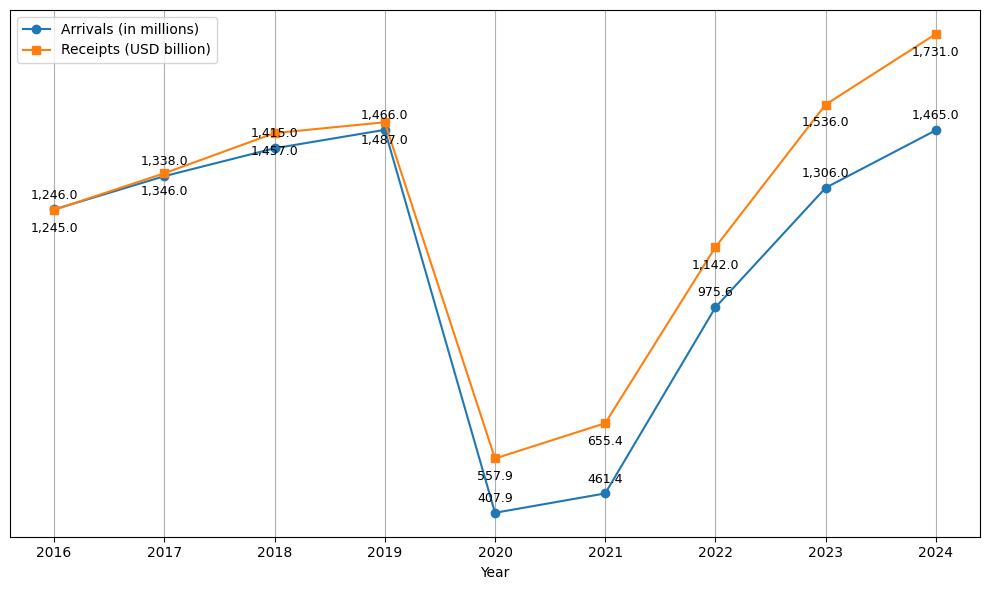
\includegraphics[width=0.9\textwidth]{Images/international_tourism_results.png}
    \captionsetup{font=footnotesize}
    \caption{\textit{International Tourist Arrivals \& Receipts. Source: UNWTO.}}
    \label{fig:global_results}
\end{figure}

\indent Moreover, Ascoli Piceno, a historic city located in the Marche region of central Italy and known for its rich cultural heritage, well-preserved medieval architecture, and local traditions \cite{italia_it}, serves as a useful reference case for this thesis, which aims to develop an efficient analytical method for the tourism sector capable of producing reliable results through the identification of the most relevant attributes. Although it remains a small destination in terms of total arrivals, Ascoli Piceno has shown steady growth and clear potential for further development within the national tourism landscape. This highlights its marginal role in the Italian tourism market, despite its rich cultural and historical appeal, and reinforces the need to explore what types of tourists might be interested in discovering lesser-known destinations like Ascoli Piceno, and how they might differ from visitors to Italy’s more popular cities \cite{istat}.

\section{Previous Work}

\indent This research originates from a project initially developed for the Marketing Analytics course within the Master’s Degree in Data Science for Economics, for the academic year 2024/2025, at the Università degli studi di Milano. The project had a similar objective to the present work, but was carried out over a shorter time period and primarily aimed at applying the techniques taught during the course, not too focused on delivering an in-depth analysis to the city. The course had a duration of almost 3 months, and the project had a duration of around 1 month. In view of this, the earlier project presented several limitations, apart from the short timeframe, which are addressed differently and in greater depth in the current thesis.

\indent First, there was a significant limitation in the qualitative interviews conducted during the initial stage of the project (see Appendix~\ref{sec:previouswork} for an example of these interviews). The main objective of these interviews was to collect qualitative data about participants’ tourist behaviour, which would then serve as the basis for defining the final attributes to be analysed in the quantitative survey. The main limitation was that the interviews contained a small number of predefined questions that were very specific, leaving little room for respondents to describe their genuine behaviour in a tourist destination. Moreover, this limitation may have resulted in the omission of potential attributes that could have further enriched the study. These ``open" questions were formulated so narrowly that interviewees often provided very short answers. Furthermore, the interviews lacked questions related to actual travel experiences, which resulted in a generalised understanding of certain tourist topics rather than experience-based insights.

\indent Second, after the qualitative interviews stage, came the definition of the main attributes. This phase also had its limitations regarding the project’s main goal, as it defined very general attributes (see Appendix~\ref{fig:pw_attributes}). Such generalization led to a limited analysis of tourist behaviour, mainly because attributes such as price, food, culture, and accessibility, among others, did not clearly describe specific tourist behaviours, and failed to describe important aspects that Ascoli Piceno could focus on. For instance, the attribute price could refer to food prices, accommodation costs, transportation costs, or even event ticket prices, among others. Moreover, attributes such as price may have been interpreted in opposite ways by different types of respondents (e.g. budget vs premium travellers), leading to answers that looked equally important but for contradictory interpretations. This ambiguity prevented the attributes from effectively discriminating across tourist segments. In addition, most of the interviews were not recorded, so the final transcriptions relied on the interviewer’s notes, making it impossible for other team members to verify them and maybe extract more valuable insights. Furthermore, no subsequent step was carried out to reinforce or validate the defined attributes, such as an explanatory or follow-up survey that could have complemented the qualitative interviews and refined the attribute selection. Although the project’s final outcome was sufficient for the course's goal, the definition of attributes could have been improved to achieve more precise and insightful results.

\begin{figure}[H]
    \centering
    
\includegraphics[width=0.5\textwidth]{Images/pw_attributes.png}
    \captionsetup{font=footnotesize}
    \caption{\textit{Previous Work Attirbutes. Source: Author’s own elaboration.}}
    \label{fig:pw_attributes}
\end{figure}

\indent Third, the following stage was the online survey, which aimed to obtain quantitative data for the final results and analysis. Although the outcomes were satisfactory and considered sufficient for the course’s objective, the total number of responses (80) was relatively low. A larger and more diverse sample would have further strengthened the validity and generalizability of the results. On the other hand, some questions could have been removed because they were already covered by others, or did not contribute at all. For example, respondents from Italy were asked an additional question: ``From which Italian region are you?". This question not only failed to add value to the analysis but was not even used. Another example is the question ``How far would you be willing to travel for a weekend getaway?", which aimed to assess the distance that respondents were willing to travel over a weekend. The main issue here was that the question assumed a short trip, thereby excluding the possibility of longer journeys, and again it did not add meaningful value due to its specificity. Another limitation of this survey was that most questions did not allow for a deeper exploration of attributes. Although there were questions designed to obtain a good description of each cluster, they failed to provide further insight into the rationale behind the order in which respondents ranked the attributes. Additionally, some of the collected data appeared rather noisy, which complicated the possibility of deriving robust clusters. For instance, repeated applications of clustering validation techniques (such as KElbowVisualizer) yielded unstable and inconsistent results, suggesting that the attributes were not sufficiently discriminative. This issue was further amplified by the role of respondents’ imagination: answers could vary depending on who planned the trip, the season, or the travel companions, which are factors that were not controlled in the survey.

\indent Following the online survey, several questions related to Van Westendorp’s Price Sensitivity Meter, explained in detail in chapter 3, were included. These questions targeted very specific cases, such as the Quintana event, the Ascoliva Festival, a wine tasting, and a city tour. However, the model is designed to estimate willingness to pay for a representative product within the target market. \cite{vw_model}. A more appropriate approach would have been to formulate a single, general question referring to a typical tourist package, in order to obtain results that are more representative and comparable.

\indent Fourth, the project was conducted as a group assignment, mainly during the winter break, which created challenges in terms of coordination. Each member faced different personal contexts: some were engaged with other courses and examinations, while others were travelling to their home countries. As a result, finding common times for meetings was often difficult, and the overall progress of the work advanced more slowly than expected.

\indent Last but not least, the survey was written exclusively in English, which excluded some potential respondents who spoke Spanish, the third most widely spoken language in the world and commonly used across many regions. Although English is often regarded as a universal language, providing a Spanish version could have increased participation, particularly among older individuals less familiar with English. This would have enriched the dataset by incorporating perspectives from a group that may have distinct travel behaviours and preferences.

\indent In summary, while the original project successfully met the requirements of the course and provided an initial exploration of the research topic, these limitations constrained the depth, precision, and representativeness of its findings. The present thesis builds upon that foundation, addressing them through a more extensive working time period, improved qualitative methods, a refined survey design, and a larger and more diverse sample.


\chapter{Literature Review}

\indent This chapter reviews the main literature that supports and informs this research. It presents studies that explain the main ideas, theories, and methods relevant to this work. The aim is to show what has been done in previous research and to provide the theoretical and methodological background for the present study.

\indent The review begins by discussing the qualitative and quantitative research approaches, outlining their key characteristics, strengths, and limitations. It then introduces major concepts and models used in tourism studies, including destination image formation and segmentation methods. This is followed by a review of quantitative techniques commonly applied in tourism research, such as discrete choice experiments and conjoint analysis, along with related issues like response-style effects and hypothetical bias that can affect data interpretation.

\indent The final part of the chapter focuses on more recent developments in the use of data-driven approaches, including text mining and data mining methods applied to customer feedback, segmentation, and product attribute analysis. These studies demonstrate how new analytical techniques can provide deeper insights into tourist preferences and decision-making patterns.

\section{Qualitative Approach}

\indent The qualitative approach relies on non-numerical evidence to generate insights and draw conclusions \cite{finnetal}. Such conclusions are based on rich, descriptive data, including words, narrative and observations, often referred to as ``soft" data \cite{mcdowell}. This method is particularly suited to the in-depth exploration of a topic and is commonly employed to understand how individuals experience and interpret the world \cite{scribbr}. It allows the identification of previously unknown processes, provides explanations of why and how phenomena occur, and reveals the range of their effects \cite{creswelletal}. In this approach, the researcher seeks to interpret situations without imposing pre-existing assumptions or expectations on the phenomenon or setting under investigation \cite{amaratunga}. 

\indent The literature also highlights several potential risks that should be considered and mitigated:

\begin{enumerate}
    \item Compliance bias: refers to situations in which participants’ responses may be influenced by their perception of what they believe is expected of them \cite{massimo}.
    \item Offset bias: occurs when participants are encouraged to reflect on issues they had not previously considered or to perceive certain topics as more complex than they would under normal circumstances \cite{massimo}.
    \item Speculation bias: arises when participants are asked to predict their own behaviour in hypothetical future scenarios. Research suggests that individuals are generally not accurate in forecasting their actions in situations they have never experienced \cite{massimo}.
\end{enumerate}

\subsection{Advantages of Qualitative Approach}

\indent The qualitative approach seeks to preserve the voice and perspective of participants and can be adapted as new research questions emerge \cite{scribbr}. It is characterised by flexible design, which allows the researcher to experiment with different techniques to determine what is most effective within the context of the project \cite{gilmore}. Furthermore, it is typically conducted in natural settings, where data collection takes place in real-world contexts or in ways that closely mirror participants’ everyday environments. This facilitates the gathering of meaningful insights by listening to detailed descriptions of people’s experiences, feelings, and opinions. Such information can help improve the design, testing, or development of systems, services, or products. In addition, using open-ended questions and flexible approaches makes it easier to come up with new ideas and discover problems or opportunities that were not expected at the start of the study \cite{scribbr}.

\subsection{Disadvantages of Qualitative Approach}

\indent On the other hand, qualitative research has several limitations. First, its real-world setting can make findings less reliable because many factors influencing the data cannot be controlled. Second, the strong role of the researcher in interpreting results introduces subjectivity, meaning the same data could be analysed differently by different people and the study cannot be exactly replicated \cite{scribbr}. This reinforces the long-standing criticism that qualitative research findings are not
verifiable, and verifiability, the principle that empirical investigations should be capable of replication so that their findings can be confirmed or refuted, is a central tenet of scientific research. It is difficult to replicate qualitative studies in the same way as quantitative ones; however, this does not mean that qualitative research entirely lacks verifiability \cite{allan}. This is why it is important for the researcher to carefully document each step of the process, thereby creating an audit trail that allows other researchers to trace and review the original procedures if needed \cite{lincoln}. Third, the use of small samples limits the extent to which results can be generalised to a broader population, even when the analysis is rigorous \cite{scribbr}. This criticism may not be entirely justified, as the generalisability of results to an entire population is rarely the primary objective of the qualitative research approach \cite{deruyter}. Finally, qualitative research can be labour-intensive, as the review and interpretation of large amounts of textual data often require manual checking, despite the availability of software tools to assist with the process \cite{scribbr}.

\section{Quantitative Approach}

\indent The quantitative approach is defined as a research strategy that relies primarily on numerical evidence to draw conclusions \cite{veal}. Because of its focus on measurement and statistical analysis, it has often been described as a ``hard" or ``number-crunching" approach to research \cite{murphyblack}. This approach involves the systematic collection and analysis of numerical data in order to identify patterns and averages, test relationships between variables, make predictions, and, when appropriate, generalise results to larger populations. It can be applied in various forms, including descriptive research, which summarises characteristics of variables; correlational research, which explores relationships between variables; and experimental research, which examines cause-and-effect links under controlled conditions. Data collection methods range from surveys and structured observations to experiments and secondary data analysis, all of which require clear operational definitions to translate abstract concepts into measurable indicators. Once collected, the data are processed and subjected to statistical analysis to answer the research questions and test the hypotheses \cite{scribbrquant}.

\subsection{Advantages of Quanitative Approach}

\indent The quantitative research offers several advantages, particularly in terms of standardisation and the potential to generalise findings to broader populations. One of its key strengths is replication, as the use of standardised data collection procedures and tangible definitions of abstract concepts allows studies to be repeated under similar conditions. This also facilitates direct comparisons of results, enabling research to be reproduced across different cultural contexts, time periods, or participant groups, with outcomes compared statistically. The accuracy of these measurement tools, such as questionnaires, can be strengthened by testing their reliability using objective measures prior to data collection \cite{neuman}. Furthermore, the approach is also well-suited to working with large samples, as quantitative data can be processed and analysed through consistent and reliable statistical procedures \cite{scribbrquant}. The knowledge gained from this group or subset of the population is representative of of the entire population under study \cite{bernard}. Finally, an additional advantage of the quantitative approach is that it is generally considered as a relatively impersonal method of conducting research, which helps to minimise the influence of the researcher’s personal biases on the outcomes of the study \cite{cooper}.

\subsection{Disadvantages of Quanitative Approach}

\indent Despite its strengths, quantitative research also has its own limitations. One of them is superficiality, as the use of precise and restrictive operational definitions may inadequately represent complex concepts. For example, an abstract notion such as ``mood" may be represented by a single numerical score, whereas qualitative research could provide a richer explanation. A narrow focus can also be an issue, since predetermined variables and measurement procedures may lead to the omission of other relevant observations. Moreover, even with standardised procedures, structural bias can occur due to factors such as missing data, imprecise measurements, or inappropriate sampling methods, which may distort the findings\cite{scribbrquant}. Finally, the quantitative approach can be relatively inflexible, as there is little a researcher can do after discovering an error in the data collection instrument. For instance, a question that is ambiguous or has been misinterpreted \cite{carsonetal}.

\section{Model of Destination Image Formation}

\indent Baloglu and McCleary’s (1999) study is one of the most influential contributions to destination image research, offering both a conceptual framework and empirical evidence on how such images are formed. Their model shifts the focus from static descriptions of image, which dominated earlier studies, to the dynamic process through which potential tourists develop perceptions and impressions of destinations, particularly when they have not previously visited. They propose that destination image is a multi-dimensional construct composed of cognitive, affective, and global components. The cognitive or perceptual dimension reflects an individual’s knowledge and beliefs about a destination’s attributes—such as infrastructure, safety, cultural attractions, and value for money. The affective dimension refers to the emotional responses a destination evokes, such as whether it feels pleasant, exciting, or relaxing. Together, these components shape the overall image, which ultimately guides destination choice \cite{destinationimg}.

\indent Destination image arises from two broad forces: stimulus factors and personal factors. Stimulus factors include external influences such as marketing communications, media portrayals, word-of-mouth, and prior experience. Personal factors, in contrast, are characteristics of the perceiver, covering sociodemographic attributes like age and education as well as socio-psychological travel motivations, such as the desire for relaxation, excitement, knowledge, social interaction, or prestige. When individuals have not yet visited a destination, three determinants are particularly important in shaping image: tourism motivations, sociodemographic characteristics, and information sources. In their model, as shown in Figure~\ref{fig:destinationimage}, information sources act as stimulus variables, while motivations and sociodemographics represent personal characteristics \cite{destinationimg}.

\begin{figure}[H]
    \centering
    \fbox{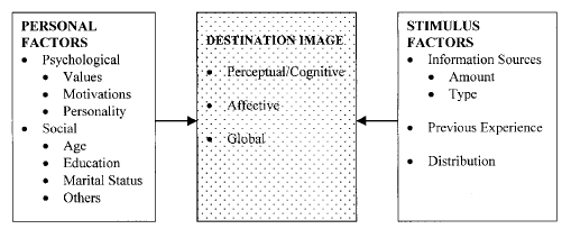
\includegraphics[width=0.8\textwidth]{Images/Destination Image.png}}
    \captionsetup{font=footnotesize}
    \caption{\textit{A General Framework of Destination Image Formation. Source: Baloglu and McCleary’s (1999).}}
    \label{fig:destinationimage}
\end{figure}

\indent To test these propositions, Baloglu and McCleary developed a path model that hypothesized causal relationships among these variables. They predicted that cognitive evaluations would significantly influence affective ones, and that both dimensions would in turn affect overall image, with affect expected to carry the stronger impact. They also proposed that the variety and type of information sources, along with age and education, would affect cognitive evaluations, while motivations would directly influence affective responses. In total, eight hypotheses were tested through path analysis, using survey data from 448 potential tourists evaluating four Mediterranean destinations (Turkey, Greece, Italy, and Egypt) \cite{destinationimg}.

\indent The findings strongly supported the proposed model. Cognitive evaluations emerged as significant predictors of affective responses, with “quality of experience” standing out as the most powerful cognitive factor shaping emotions. Affective evaluations, in turn, had the strongest direct effect on overall image, underscoring their mediating role. The study also revealed that the variety of information sources used positively influenced cognitive evaluations, while word-of-mouth proved to be the single most powerful information source. Age and education, however, showed a negative influence on cognitive evaluations, with older and more educated respondents assessing destination attributes less positively. Motivations played a weaker role overall, with only relaxation and escape motives showing a significant—though negative—relationship with affect \cite{destinationimg}.

\indent The study carries important implications for both theory and practice. Theoretically, it provides understanding of destination image by integrating cognitive and affective components into a single causal framework, showing the process to be dynamic and multi-dimensional. Practically, it reaffirms the central role of information sources, particularly word-of-mouth, in shaping perceptions, suggesting that destinations should invest in strategies that foster the sharing of positive experiences. Because motivations such as knowledge, prestige, and social interaction also influence image, marketers can adapt campaigns to tap into these psychological drivers. Finally, the negative relationship between age, education, and cognitive evaluations emphasize the need for targeted communication strategies that speak differently to diverse demographic groups. In essence, Baloglu and McCleary’s work demonstrates that destination image is co-created by external stimuli and personal characteristics, with affective responses serving as the critical bridge between cognition and overall impression \cite{destinationimg}.

\section{Segmentation and Response-Style Effects}

\indent Pesonen and Honkanen (2014) examine how tourists’ response styles can influence segmentation outcomes when applying k-means cluster analysis. A response style refers to the tendency of individuals to answer questionnaires in a systematic way that is unrelated to the actual content. For example, consistently giving high or low ratings, or avoiding the extremes of a scale. These patterns, known as response-style effects, can significantly distort cluster solutions by grouping individuals based on their answering habits rather than their true motivations or attitudes. Since segmentation aims to form clusters that are internally homogenous and externally distinct, ignoring response styles may lead to producing segments that are artificial and unhelpful for marketing purposes \cite{clustering}.

\indent The authors note that cluster analysis, particularly k-means, remains the most widely used technique in tourism segmentation research. However, this approach is highly sensitive to response styles. Past research has sometimes produced clusters resembling “want-it-all” tourists who rate everything highly, or “passive” tourists who rate everything poorly, patterns that may reflect answering tendencies rather than meaningful market segments. Such results challenge the practical utility of segmentation for identifying actionable strategies \cite{clustering}.

\indent To investigate this issue, the authors collected data via an online survey hosted on a Finnish cottage holiday website. Respondents rated 31 travel motivation items on a 7-point Likert scale. After data cleaning, 709 responses were retained, of which 25 motivation items were used for segmentation. The researchers applied k-means cluster analysis to four versions of the dataset \cite{clustering}:

\begin{enumerate}
    \item The original unstandardized data.
    \item Data adjusted to remove acquiescence response style (ARS) through within-case standardization (row-centering), which highlights relative item importance per respondent.
    \item Data adjusted to remove extreme response style (ERS) by dividing responses by each individual’s standard deviation.
    \item Data with both ARS and ERS removed.
\end{enumerate}

\indent The results revealed marked differences across the cluster solutions. Using the original data, the clusters largely mirrored response styles: some groups scored consistently high, others low, and some in the middle. This confirmed that k-means was capturing answering patterns rather than motivational differences. Once ARS was removed, however, the clusters displayed distinct motivational profiles, with respondents prioritizing certain travel motives over others. This approach produced more interpretable and actionable segmentations. By contrast, removing only ERS offered little improvement, as the clustering still reflected broad high–low patterns. When both ARS and ERS were removed, the solution resembled the ARS-only result, suggesting that acquiescence was the dominant factor influencing clustering \cite{clustering}.

\indent The study emphasizes the methodological importance of addressing response-style bias in tourism segmentation studies. Without accounting for these effects, researchers risk generating misleading clusters that do not represent real market segments. Pesonen and Honkanen conclude that correcting for ARS yields the most meaningful results in this case, and they stress the need for segmentation studies to explicitly report how response styles are handled. They further recommend that future research explore alternative segmentation methods and use simulated data to deepen understanding of how response styles shape clustering outcomes \cite{clustering}.

\section{Representing Tourists’ Heterogeneous Destination and Travel Party Choices}

\indent Wu, Zhang, and Fujiwara (2011) develop a modeling approach that jointly analyzes tourists’ choices of destination and travel party, recognizing that these decisions are interdependent and vary across individuals. Travel decisions are rarely made in isolation; the choice of destination often depends on who tourists travel with, and the composition of the travel party can influence destination selection. The authors argue that treating these choices separately, as prior studies often did, overlooks the sequential and interactive nature of travel decisions. Their paper addresses this by integrating a latent class model with a nested logit model to capture both the interdependency and heterogeneity in tourist decision-making \cite{touristheterogenity}.

\indent The latent class model identifies unobserved tourist segments that follow different decision-making sequences. Some decide on a destination first, then their travel companions, while others choose their travel party before selecting a destination. Within each segment, the nested logit model reflects the sequential choice process based on random utility maximization. This combined approach allows distinguishing groups with distinct “decision hierarchies,” offering a more realistic representation of travel behavior \cite{touristheterogenity}.

\indent The model uses survey data from over 2,000 tourists in Japan, covering 14 destination zones and three travel party categories: traveling alone, traveling with family, and traveling with friends or others. Variables influencing destination choice included travel time, destination attractiveness (measured by annual visitors), and number of tourist spots. Travel party choice was explained by gender, age, and marital status. Results showed all explanatory variables were statistically significant. Travel time had the strongest impact on destination choice, while marital status most strongly predicted travel party composition. Women and married individuals were more likely to travel with family or friends, whereas younger travelers leaned toward independent travel. Crucially, about half of tourists followed a decision sequence beginning with destination choice (latent class 1), while the other half started by selecting their travel party (latent class 2). This demonstrates the absence of a single dominant pattern and emphasizes the importance of modeling heterogeneity rather than assuming uniform behavior. The nested logit parameters confirmed significant interdependencies \cite{touristheterogenity}.

\indent The authors conclude that this integrated latent class–nested logit model provides a more flexible and realistic framework for capturing tourist decision-making. For planners and marketers, the findings highlight the value of understanding destinations’ sensitivity to travel party structure, enabling more targeted promotions. The study also points to the importance of considering decision-making structures alongside sociodemographic segmentation. The authors suggest future research should expand the model to include additional decision dimensions, such as accommodation and travel mode choices, and test its applicability across cultural contexts \cite{touristheterogenity}.

\section{Discrete Choice Experiments in Tourism}

\indent Kemperman (2021) provides a comprehensive review of the use of discrete choice experiments (DCEs) in tourism, analyzing 49 studies published between 2010 and 2020 in the five leading tourism journals. DCEs are widely employed to measure and predict preferences by presenting individuals with alternatives that vary in their attributes. This approach allows researchers to estimate the relative importance of different destination, product, or service features and to calculate willingness to pay for specific attributes. In tourism, DCEs have been applied to questions such as destination choice, travel mode, accommodation type, and activity selection \cite{discretechoice}. 

\indent The method is rooted in random utility theory, which assumes that individuals choose the option that maximizes their utility. Utility consists of a systematic component, based on observable attributes, and a random component that captures unobserved factors. In tourism, this means that travelers are assumed to select the destination, activity, or service that provides the highest perceived benefit given their motivations and constraints. By putting together destinations or services as bundles of attributes such as price, quality, amenities, and location, and asking respondents to choose between hypothetical alternatives, researchers can estimate the marginal utility of each attribute \cite{discretechoice}.

\indent DCEs can use both revealed and stated choice data. Revealed data come from actual behavior such as bookings, while stated data are gathered in controlled experiments. The former reflects real-world decisions, whereas the latter allows researchers to anticipate preferences for products or services that do not yet exist. In practice, when market data are unavailable or lack variation, stated choice experiments often provide the only viable means of capturing likely behavior \cite{discretechoice}.

\indent A key strength of DCEs is their ability to simulate decision-making in a structured way. Tourists are presented with multiple choice scenarios in which attributes vary systematically, allowing researchers to isolate the impact of each factor. This design provides high internal validity, though external validity can be more limited since the choices are hypothetical. Kemperman’s review shows that most studies still examine single, independent decisions but relatively few investigate linked or sequential decisions, such as destination, transport, and accommodation together. In reality, these choices are interdependent \cite{discretechoice}.

\indent Kemperman (2021) shows that discrete choice experiments provide a powerful lens for understanding tourist preferences and predicting responses to innovations in tourism products and services. She argues that future research should design more realistic experiments, incorporate dynamic needs and social influences, and make use of emerging tools such as virtual reality and eye-tracking to enhance engagement and data quality. Such advancements would extend DCEs beyond predicting what choices tourists make toward offering richer insights into how and why those choices are made \cite{discretechoice}.

\section{Conjoint Analysis in Tourism}

\indent Altin (2023) offers a comprehensive overview of how conjoint analysis has been applied in tourism research as a method for measuring tourist preferences. Conjoint analysis is a choice-based technique that allows researchers to understand how travelers value different attributes of destinations, services, or experiences. By decomposing a tourism product into key elements, such as price, accommodation type, attractions, or amenities, it estimates the value respondents assign to each attribute. This makes it possible to capture the trade-offs travelers are willing to make when choosing between alternatives, providing useful insights for destination management organizations (DMOs), tour operators, and other industry stakeholders seeking to design competitive offerings \cite{conjointaltin}.

\indent Methodologically, conjoint analysis involves presenting respondents with sets of hypothetical profiles or “bundles” that combine different attribute levels. Respondents are asked to select their preferred option from each set. Statistical analysis of these choices produces utilities and relative importance estimates for each attribute, showing which features drive satisfaction and willingness to pay (WTP). In tourism, this approach has been applied to diverse products such as destination packages, activity mixes, accommodation types, and other experience-based offerings. Given that tourism products are typically multi-attribute in nature, conjoint analysis provides a structured way to reflect their combined influence on decision-making \cite{conjointaltin}.

\indent Altin (2023) \cite{conjointaltin} also highlights the practical advantages of conjoint analysis for industry practitioners. Well-designed studies can guide product development and market positioning by identifying which attributes matter most to particular traveler segments. By simulating realistic decision-making, conjoint analysis also supports market segmentation, differentiation, and competitive benchmarking, which are critical in a crowded and highly competitive industry \cite{conjointaltin}.

\indent The author also describes several considerations and challenges in applying conjoint analysis. First, the careful selection of attributes is essential: including too many risks overwhelming respondents, whereas omitting key features may reduce validity. Second, samples must be sufficiently representative to ensure generalizable results. Altin further notes the growing relevance of digital and adaptive conjoint approaches, which ease data collection and allow more flexible, personalized designs. As tourism evolves toward increasing complexity, through sustainability concerns, digital innovations, and shifting traveler expectations, conjoint analysis continues to adapt in order to capture these new dimensions of tourist choice \cite{conjointaltin}.

\indent Altin’s work serves as a methodological anchor in tourism research by demonstrating the value of conjoint analysis for understanding preferences, informing product design, and supporting strategic decisions at both managerial and policy levels. By linking conjoint studies with broader frameworks of tourism behavior, this contribution provides a roadmap for integrating preference modeling into the study of tourist decision-making \cite{conjointaltin}.

\section{Hypothetical Bias}

\indent Hensher (2010) reviews how hypothetical bias affects willingness-to-pay (WTP) estimates derived from stated preference (SP) methods and discrete choice experiments (DCEs). Hypothetical bias arises from discrepancies between what people report they would choose or pay in surveys, and what they actually do in real-world situations. Since SP and DCE studies typically lack financial consequences, respondents may overstate their preferences or WTP, often producing inflated values. This poses a serious challenge in transport, environmental, and tourism research, where WTP estimates are commonly used to justify policies and investments \cite{hypotheticalbias}.

\indent The paper synthesizes evidence comparing WTP from hypothetical surveys with values obtained from revealed preference (RP) studies or actual market behavior. Some studies detect no difference, while others find that WTP from SP and DCEs tends to be much lower than real-market values. Hensher (2010) \cite{hypotheticalbias} argues that no single factor explains this variation and that outcomes depend on the type of good, survey design, and respondents’ familiarity with the decision context \cite{hypotheticalbias}.

\indent To mitigate hypothetical bias, several strategies are discussed. One is anchoring surveys in real experiences, for example by “pivoting” choice sets around respondents’ existing travel habits. This grounds choices in familiar conditions, and narrows the gap between hypothetical and real decisions. Other techniques include adding opt-out alternatives, using “cheap-talk” scripts that warn about overstatement, or providing consequentiality scripts and honesty oaths to increase the perceived importance of responses. While these tools have shown promise, their effectiveness is context-dependent \cite{hypotheticalbias}.

\indent The author also highlights the role of calibration methods. Ex ante approaches (instrument-based) seek to prevent bias during survey design, while ex post techniques (statistical adjustments) correct results after data collection using confidence ratings or benchmark comparisons. For instance, calibration functions derived from observed market data have been applied to adjust WTP values, producing results more consistent with revealed behavior \cite{hypotheticalbias}.

\indent A key contribution of the paper is its emphasis on reference alternatives in DCEs. Anchoring choice tasks to respondents’ actual experiences, rather than purely hypothetical scenarios, was shown to reduce bias. Case studies in Australia and New Zealand demonstrated that mean values of travel time savings (VTTS) were significantly higher and more realistic when based on a reference commute compared to forced-choice scenarios. This suggests that reference-dependent designs yield WTP estimates that are more reliable for policy analysis \cite{hypotheticalbias}.

\indent Hensher (2010) \cite{hypotheticalbias} concludes that no universal remedy exists for hypothetical bias. Instead, researchers should use a combination of careful survey design, calibration techniques, and validation against real behavior. The paper highlights the need for further research into hybrid data approaches and pivot-based experiments, which show strong potential for narrowing the gap between hypothetical and real-world valuations \cite{hypotheticalbias}.

\section{A Text Mining Based Approach for Mining Customer Attribute Data on Undefined Quality Problems}

\indent Zhu, Li, and Wu (2018) address the challenge of understanding customer perceptions of quality issues that are not easily defined through traditional evaluation methods. As market structures become increasingly complex, conventional tools such as SERVQUAL often fail to capture the full scope of customer concerns or provide actionable insights. To overcome this limitation, the authors propose an unsupervised machine learning text-mining approach combined with a Recursive Neural Tensor Network (RNTN) to extract customer attribute data from unstructured textual sources \cite{textmining}.

\indent Their framework focuses on the consumer perspective, demonstrating that customers exhibit a coherent “line of sight” when identifying quality problems, even when their feedback involves diverse and scattered attributes. The text-mining process enabled the identification of attribute clusters and revealed that approximately 61\% of consumers converge on common strategies to address ambiguous quality issues through collective reasoning \cite{textmining}.

\indent The study illustrates how advanced text-mining techniques can uncover hidden patterns in consumer feedback that traditional survey-based methods may overlook. By leveraging large volumes of unstructured customer data, this approach provides managers with data-driven insights into quality perception, thereby enhancing quality management and the detection of subtle or emerging concerns \cite{textmining}.

\section{Text Mining for Product Attribute Extraction}

\indent Ghani et al. (2006) propose a method for extracting attribute–value pairs from textual product descriptions to enrich product databases. By conceptualising products as collections of attributes and values rather than as atomic entities, their approach improves the performance of applications such as demand forecasting, assortment optimisation, and product recommendation systems. The study addresses both explicit physical attributes (e.g., size, colour) and implicit semantic attributes (e.g., trendiness, brand appeal), focusing primarily on products in the apparel and sporting goods industries \cite{ghani}.

\indent The authors formulate attribute extraction as a classification problem and employ a semi-supervised learning approach that requires minimal labelled data. Their model leverages large quantities of unlabelled text through co-training and dependency parsing to accurately identify relationships between attributes and their corresponding values. Furthermore, expert discussions informed the identification and categorisation of attributes according to explicit and semantic characteristics \cite{ghani}.

\indent The proposed system’s modular architecture—comprising data collection, seed generation, attribute extraction, value relationship extraction, and user interaction—enhances both scalability and adaptability. Experimental results demonstrate strong accuracy in extracting attribute–value pairs, thereby facilitating the expansion, enrichment, and analytical use of large-scale product attribute databases \cite{ghani}.

\section{Data Mining on Customer Segmentation: A Review}

\indent Kaur and Kaur provide a comprehensive review of data mining techniques applied to customer segmentation, a fundamental process for dividing customers into meaningful groups based on shared characteristics. The paper emphasises the strategic importance of segmentation in modern marketing and customer relationship management, as it enables organisations to tailor their offerings and communication to the specific needs of each segment \cite{datamining}.

\indent The authors examine a range of clustering algorithms, including K-means, DBSCAN, and fuzzy C-means, outlining their respective advantages and limitations in identifying distinct customer groups. They stress that effective segmentation depends on forming clusters that are internally cohesive yet externally distinct, while maintaining relevance to real-world customer profiles \cite{datamining}.

\indent Beyond traditional clustering, the review explores advanced machine learning approaches, such as neural network–based predictive models that leverage product reviews, purchase behaviour, and temporal data to improve segmentation precision. The authors also highlight the role of feature extraction techniques—including unigram, bigram, and trigram analysis—in capturing customer sentiment and preferences from textual data \cite{datamining}.

\indent Overall, the study demonstrates that the careful application of data mining techniques can yield valuable insights into customer behaviour, supporting the development of more targeted marketing strategies and enhancing customer satisfaction \cite{datamining}.

\section{Unlocking insights: integrated text mining and interpretive structural modeling for enhanced user review analysis}

\indent Li, Liu, and Chen (2024) propose a novel approach that integrates text mining with Interpretive Structural Modeling (ISM) to analyse large volumes of user-generated reviews, enabling manufacturers and e-commerce platforms to better understand customer preferences and behaviours. The study applies two text mining techniques—TF–IDF and Word2Vec—to extract meaningful keywords and explore semantic relationships within review texts. The extracted insights are visualised through knowledge graphs constructed using Neo4j, allowing the identification and exploration of thematic connections within the data \cite{unlockinginsights}.

To further extend the analysis, the authors employ ISM to reveal hierarchical and interdependent relationships among key product attributes derived from the reviews. Using a dataset of milk product reviews from Suning.com, six major elements influencing user feedback were identified: freshness of taste, discounted prices, logistics, customer repurchase, product packaging, and nutritional composition. These attributes were organised into three hierarchical layers representing their relative influence—discounted prices, repurchase, and logistics at the top; packaging and nutritional composition in the middle; and freshness of taste as the foundational factor \cite{unlockinginsights}.

This integrated text mining-ISM framework improves the depth and interpretability of user review analysis by capturing both semantic meaning and structural relationships among attributes. The study demonstrates the potential of combining quantitative text analytics with structural modeling to generate actionable insights for product development, marketing optimisation, and consumer experience enhancement \cite{unlockinginsights}.


\chapter{Methodology and Results}

Add an introduction to the chapter

\section{Qualitative Interviews}

\subsection{Methodology}

\subsubsection{The Interviews}

\indent The first step consisted of qualitative interviews, which were used to identify possible attributes related to tourist destinations. This was carried out through flexible open questions, mainly focusing on real-world experiences. Although flexible, a guide of predefined questions was created (see Figure~\ref{fig:qualitativeguide}) to provide a general structure for the interviews, while still leaving the possibility to deviate and follow the flow of each individual conversation. Each new interview generated additional ideas and opportunities that informed subsequent ones, thus enriching the insights obtained. Furthermore, all interviews were conducted online and recorded, and the corresponding transcriptions were produced (see Appendix~\ref{sec:interview} for an example), allowing the subsequent analysis to be validated against the original data.

\begin{figure}[ht]
    \centering
    \fbox{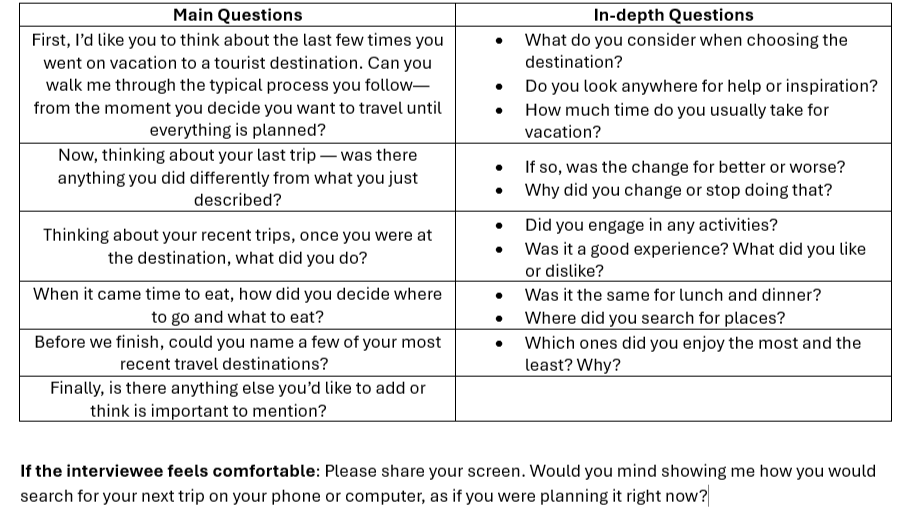
\includegraphics[width=0.9\textwidth]{Material/2. Interviews & Surveys/1. Qualitative Interview/Qualitative Interview Questions.png}}
    \captionsetup{font=footnotesize}
    \caption{\textit{Guide for Qualitative Interview Questions. Source: Author’s own elaboration}}
    \label{fig:qualitativeguide}
\end{figure}

\indent For these interviews, the aim was to gather perspectives from individuals of different generations, nationalities, and professional backgrounds. The sample included:

    \begin{itemize}
        \item Sex: 8 males and 2 females
        \item Age: median of 26 years old, with a maximum equal to 41 years old, and a minimum equal to 21 years old.
        \item Nationalities: 5 Argentinians, 2 Spanish, 1 Italian, 1 Colombian, and 1 Iranian.
        \item Occupations: 5 employed people and 5 Master's students (one of whom had worked for approximately 20 years before starting the degree).
    \end{itemize}

\indent The interviews were conducted through the Zoom platform and in the original language of each interviewee, allowing them to clearly and fully describe their real experiences. In cases where the interviewer and interviewee did not share the same mother tongue, English was used as the common language. Among all the interviews, the only one conducted in English was with the Iranian participant. Furthermore, all interviewees were informed about the recording process, with emphasis placed on the fact that no personal or sensitive information would be disclosed. The main objective at this stage was to understand the genuine process by which interviewees defined and prepared a trip. For this reason, participants were asked to share their screen (or, in cases where this was not possible, the interviewer shared the screen and followed the steps as described by the interviewee) and to demonstrate step by step how they organised either a past trip or an upcoming one. While describing their planning process, they showed the resources they used and expressed both positive and negative impressions. When needed, the interviewer intervened to ask additional questions in order to explore certain topics in greater depth. Nevertheless, the main goal was to allow the interviewee to speak as freely as possible, and as mentioned before, without introducing any potential bias.

\indent After this initial block, in which participants described their real-life experiences of trip planning, they were asked specifically about Ascoli Piceno. In this section, they were invited to demonstrate how they would prepare for a hypothetical trip to the city. They were asked to apply their usual, real-life trip planning process to the case of Ascoli Piceno, following the same steps, tools, and resources they normally use. The aim was to capture their genuine opinions about Ascoli Piceno and to identify potential attributes associated with it, both positive and negative. One of the most relevant aspects of this stage concerned their impressions when analysing the map and the geographical position of the city. In some cases, participants were also asked to compare Ascoli Piceno with Pistoia, a city of similar characteristics located near Florence. At this point, further attributes emerged, particularly when interviewees were asked to decide whether they would prefer to visit one city over the other, and to explain their reasons.

\indent Finally, they were introduced to specific topics related to Ascoli Piceno, such as the olive ascolane and the Quintana festival, in order to gather insights about attributes associated with local events and cultural traditions. At the end of the interview, participants were given the opportunity to add any further comments, which often provided additional perspectives or reinforced the main points that had emerged throughout the session.

\subsubsection{Manual Attribute Identification}

\indent After all interviews were completed, the transcription cleaning process was carried out. For the first two interviews, since the automatic transcription feature had not been enabled, the audio files were transcribed in Google Colab using \texttt{WhisperX}, an enhanced transcription tool built on OpenAI’s Whisper that incorporates speaker diarization from Hugging Face to provide more accurate transcripts and speaker separation \cite{whisperx}. Once the raw transcriptions were obtained (either from Google Colab or Zoom), a manual verification process was conducted. During this stage, the transcripts were checked against the recordings and corrected where necessary, particularly in cases where words or phrases had been inaccurately transcribed. Finally, ChatGPT was used carefully to efficiently translate each transcription into English.

\indent Following the transcription cleaning process, each transcription was carefully re-read, with notes taken on the most relevant insights and linked to potential attributes. This process was repeated for every interview, highlighting key phrases and extracting attributes. Once this analysis was completed, all unique attributes were compiled in an Excel sheet together with their corresponding frequency. Frequency was defined as the number of interviews in which a given attribute appeared, with a maximum possible frequency of 10 (equal to the total number of interviews).

\subsubsection{Text Mining and Topic Modeling Process}

\indent Complementing the previous manual analysis, a text mining process was conducted in Google Colab to reinforce the previously identified attributes and to determine whether any additional attributes could be extracted. Before proceeding with the analysis, a preprocessing stage was required. First, the Colab notebook was connected to the Google Drive account to access the raw interview transcripts. Each transcript was then cleaned through Python, by removing all interviewer segments, deleted metadata sections such as “Interviewee’s information,” and retained only the text spoken by the interviewee. Additional formatting operations were applied to remove redundant blank lines and extra spaces, ensuring a consistent and readable structure across all files. Once all transcripts were cleaned, the script automatically saved the processed versions in the same folder with a new filename prefix to distinguish them from the originals. Subsequently, another function imported all the cleaned files and concatenated them into a single DataFrame named \texttt{df\_interviews}. This consolidated dataset served as the input for the text mining stage.

\indent For the text preprocessing stage, the English language model \texttt{en\_core\_web\_sm} from the \texttt{spaCy} library was employed for text processing. The Named Entity Recognition (NER) and syntactic parsing components were disabled to improve processing efficiency, as they were not required for this analysis. With this configuration, Algorithm~\ref{alg:textpipeline} (see Appendix~\ref{sec:textmining}) was implemented. In this algorithm, each text was first converted to lowercase, and all characters that were not letters, numbers, or whitespace were removed using regular expressions. The cleaned text was then passed to the \texttt{spaCy} NLP model, which performed tokenisation. Finally, if the parameter \texttt{stopwords} was set to ``Yes,” only alphabetic tokens that were not stopwords were retained, and each token was replaced by its lemma (i.e., the base or dictionary form of the word). Although the resulting dataset (\texttt{df\_cleaned\_interviews}) was ready for analysis, a final manual adjustment was performed to remove filler words that did not provide analytical value and were not captured as stopwords, such as ``yes”, ``yeah”, ``yea”, ``uh”, ``um”, ``okay”, ``ok”, ``like”, ``dont”, ``didnt”, ``know”, ``thing”, ``things”, ``go”, ``get”, ``got”, ``just”, ``maybe”, ``kinda”, ``kind”, ``sorta”, ``mean”, ``ve”, and ``think.”

\indent Following text preprocessing, the cleaned tokens were transformed into numerical features using the Term Frequency–Inverse Document Frequency (TF–IDF) method, implemented through the \texttt{TfidfVectorizer} from the \texttt{scikit-learn} library. This approach quantifies the relative importance of each term across the collection of interviews, balancing its frequency within a document against its occurrence across all documents. All unigrams (single words), bigrams (two-word sequences), and trigrams (three-word sequences) were extracted using Algorithm~\ref{alg:compute_tfidf_ngrams} (see Appendix~\ref{sec:textmining}). The TF–IDF scores were aggregated across all documents to obtain a global measure of each term’s relative importance. To visualise the most relevant words in the corpus, a word cloud was generated for each case (single words, 2-grams, and 3-grams) using the \texttt{WordCloud} library, where word size corresponds to cumulative TF–IDF scores.

\indent For the topic modelling stage, the \texttt{BERTopic} framework was employed, combining transformer-based embeddings with clustering and class-based TF–IDF representations. Prior to model training, each interview transcript was divided into smaller textual segments to improve topic coherence. The segmentation was performed using the \texttt{chunk\_text} function (see Algorithm~\ref{alg:chunktext} in Appendix~\ref{sec:textmining}), which tokenises each text into sentences using the \texttt{sent\_tokenize} function from the \texttt{NLTK} library and then groups them into chunks of six sentences each. Only chunks longer than 30 characters were retained, resulting in a list of textual segments (\texttt{documents}) and their corresponding indices (\texttt{origin}). Sentence embeddings were then generated using the \texttt{all-MiniLM-L6-v2} model from the \texttt{SentenceTransformer} library, which encodes each chunk into a dense semantic vector. These embeddings were subsequently used as input for the \texttt{BERTopic} model, which clusters semantically similar texts and derives interpretable topic representations. This step enabled the identification of latent themes across participants’ narratives, complementing the manual attribute extraction phase.

\indent To refine the topic extraction process, a custom stopword list was defined by combining the default English stopwords from the \texttt{scikit-learn} library with domain-specific filler words and non-informative tokens (``like”, ``yeah”, ``really”, ``actually”, ``basically”, ``um”, ``uh”, ``ok”, ``okay”, ``sort”, ``kind”, ``thing”, ``things”, ``so”, ``just”, ``well”, ``yes”, ``no”, ``don”, ``dont”, ``doesnt”, ``didnt”, ``im”, ``ive”, ``youre”, ``its”, ``id”, ``think”, ``know”, ``mean”, ``look”, ``get”, ``got”, ``going”, ``go”, ``place”, ``places”, ``city”, ``cities”, ``tourist”, ``tourists”, ``trip”, ``travel”). The \texttt{TfidfVectorizer} was configured to ignore tokens shorter than four letters and to discard words appearing in fewer than two documents. Additionally, the \texttt{KeyBERTInspired} representation model was applied to enhance topic interpretability through keyword relevance weighting.

\indent The final model (see Algorithm~\ref{alg:bertopic} in Appendix~\ref{sec:textmining}) was implemented with the parameters \texttt{low\_memory=True} and \texttt{min\_topic\_size=8} to enhance computational efficiency and ensure that each topic contained a sufficient number of documents. The model was subsequently trained using the segmented documents and their corresponding embeddings, producing a set of topics (\texttt{topics}) and associated probabilities (\texttt{probs}) that represent the distribution of topics across all text segments.

\subsubsection{Complementary Attribute Discovery through ChatGPT}

\indent Before proceeding to the next step, ChatGPT was also employed as a complementary tool to identify potential attributes by providing each interview transcription separately. The prompts (see Appendix~\ref{sec:chatgpt_prompts}) were designed and implemented in two stages: first, to obtain an initial list of attributes, and subsequently, to refine and consolidate the results.

\subsection{Results}

\subsubsection{Manual Attribute Identification}

\indent After the interview transcriptions were properly cleaned, the main insights were extracted from each case (see Appendix~\ref{sec:interviewnotes}). Some phrases contained a single attribute, while others referred to multiple ones. For instance, in the first interview with the Italian respondent, he said: “…in that famous Tuscany trip, we also included the Palio di Siena…”. This was linked to a general attribute: local events. On the other hand, in the second interview with an Argentinian respondent, he said: “…we looked a lot into what the transportation is like there, food prices, which beaches are recommended.”. In this case, the phrase was related to three attributes: public transportation, food prices, and beaches. These initial attributes were not definitive but rather a starting point (see Figure~\ref{fig:attributesfreq} in Appendix~\ref{sec:manual_att}).

\subsubsection{Text Mining and Topic Modeling Process}

\indent Regarding the text mining analysis, the TF–IDF results provided valuable insights for refining and validating the list of attributes. Among the different n-gram configurations tested, the 3-grams (sequences of three consecutive words) produced the most meaningful expressions (see Figure~\ref{fig:int3wordcloud}), allowing a clearer identification of recurring concepts and patterns relevant to tourist preferences. These multi-word combinations helped to capture contextual nuances that single words or bi-grams could not, thereby contributing to a more accurate definition of the attributes. As illustrated in the following figure, the main terms and phrases extracted through TF–IDF analysis were closely aligned with the attributes identified in the previous manual stage, confirming the consistency and robustness of the attribute selection process.

\begin{figure}[ht]
    \centering
    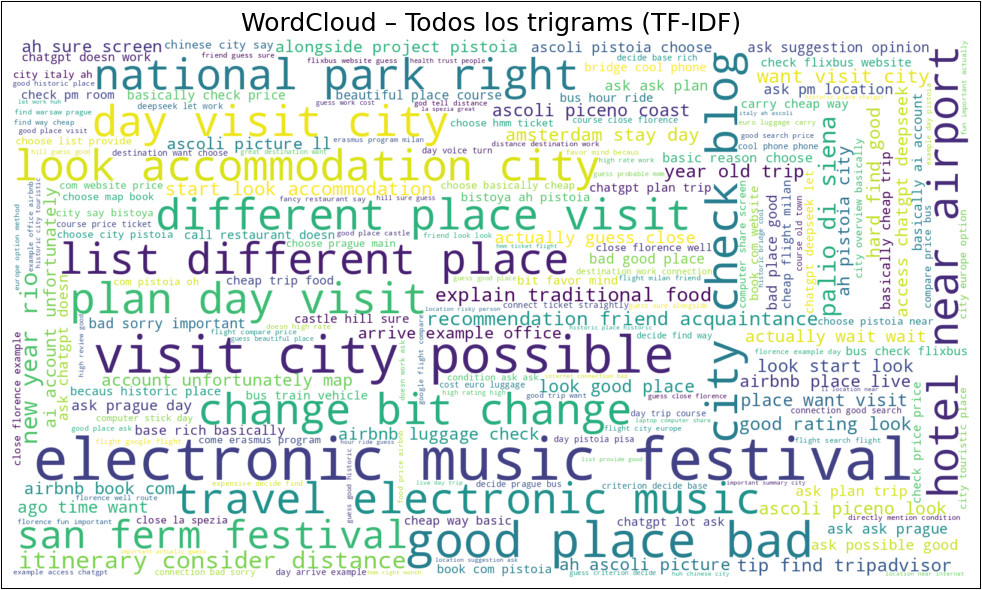
\includegraphics[width=0.9\textwidth]{Images/Qualitative Interviews/3-grams.png}
    \captionsetup{font=footnotesize}
    \caption{\textit{3-grams Wordcloud for Interviews. Source: Author’s own elaboration}}
    \label{fig:int3wordcloud}
\end{figure}

\indent The topic modeling analysis revealed distinct thematic clusters that illustrate how travelers plan and experience their trips. Overall, the model identified eight coherent clusters representing key aspects of travel behaviour and preferences, as shown in Figure~\ref{fig:bertopic}. Several clusters underscored the strong influence of digital discovery tools, as participants frequently mentioned using platforms such as Google and TripAdvisor as their primary sources of inspiration and information (Cluster 0: Digital Search \& Food Inspiration). Culinary experiences, scenic beauty, and iconic landmarks emerged as central motivations, reflecting travelers’ emphasis on authentic local food and visually appealing destinations (Cluster 1: Iconic Attractions \& Scenic Destinations).

\indent Financial considerations also played a critical role, with travelers demonstrating a clear preference for budget-conscious accommodation options such as hostels and Airbnb (Cluster 2: Budget-Friendly Lodging), as well as the systematic comparison of hotel offers and travel costs (Cluster 4: Hotel Comparison \& Budget Planning). The analysis further revealed a tendency toward multi-city itineraries and structured travel planning, where visitors combine well-known destinations with smaller towns or day trips to optimise time and variety (Cluster 3: Structured Tours \& Multicity Itineraries; Cluster 5: Short Excursions from Urban Hubs).

\indent In addition, certain clusters captured more specific travel patterns, such as the popularity of classic European city tourism focused on emblematic destinations (Cluster 6: Classic European City Tourism), and a broader category encompassing general travel exploration and destination diversity (Cluster 7: General Travel Exploration \& Destination Variety).

\indent Taken together, these clusters highlight the main drivers of contemporary travel behaviour: digital research, cost optimisation, local immersion, and multi-destination planning.

\begin{figure}[ht]
    \centering
    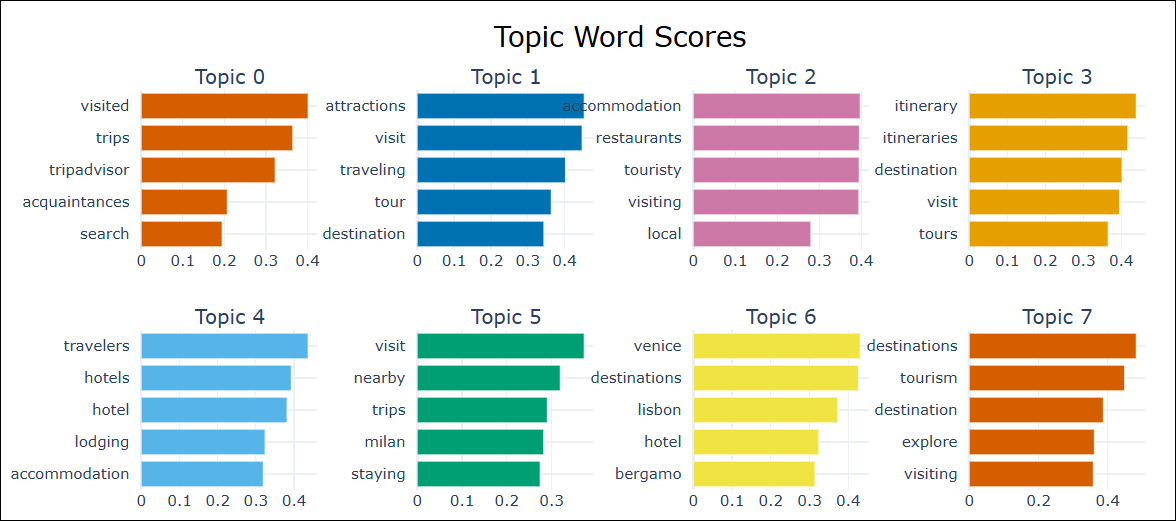
\includegraphics[width=1\textwidth]{Images/Qualitative Interviews/BERTopic.png}
    \captionsetup{font=footnotesize}
    \caption{\textit{BERTopic Clusters. Source: Author’s own elaboration}}
    \label{fig:bertopic}
\end{figure}

\subsubsection{Complementary Attribute Discovery through ChatGPT}

\indent The first attributes suggested by ChatGPT, as shown in Figure~\ref{fig:chatgpt_I} (Appendix~\ref{sec:chatgpt_att}), were relatively broad and generic, often referring to general aspects of tourism such as “food,” “culture,” or “accommodation.” While these terms reflected relevant dimensions of the travel experience, their lack of specificity risked creating conceptual overlap and ambiguity among categories. After applying the refinement prompt, the output became more detailed and contextually accurate. ChatGPT provided clearer, more actionable attribute definitions:

\begin{figure}[ht]
    \centering
    
\includegraphics[width=0.5\textwidth]{Images/Qualitative Interviews/ChatGPT_II.png}
    \captionsetup{font=footnotesize}
    \caption{\textit{Refined Attributes from ChatGPT. Source: ChatGPT}}
    \label{fig:refinedchatgpt}
\end{figure}

\subsubsection{Final Attributes}

\indent Finally, the list of attributes was refined to enhance their accuracy and clarity. Several attribute names were adjusted to prevent ambiguity or misinterpretation. Supported by the results of the text mining analysis and the complementary suggestions provided by ChatGPT, the final ten attributes were carefully selected to ensure they were representative, clearly defined, and free from ambiguity or overlap.

\begin{figure}[ht]
    \centering
    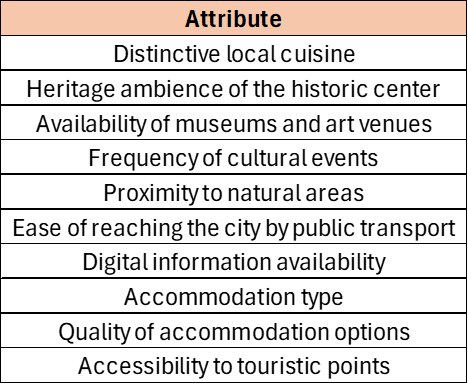
\includegraphics[width=0.4\textwidth]{Images/Qualitative Interviews/10_attributes.png}
    \captionsetup{font=footnotesize}
    \caption{\textit{Preliminary 10 attributes. Source: Author’s own elaboration}}
    \label{fig:preliminaryatt}
\end{figure}


\section{Text Mining of Online Accommodation Reviews}

\subsection{Methodology}

\indent One of the datasets used for this analysis consisted of Airbnb reviews from various Italian cities. These data were obtained from the Inside Airbnb platform, which provides quarterly datasets for multiple regions and cities available for free download \cite{airbnbdata}. The Italian cities included in this analysis were Bergamo, Bologna, Florence, Milan, Naples, Puglia, Rome, Sicily, Trentino, and Venice. All individual datasets were concatenated into a single dataset, resulting in a total of 7,141,844 records. The dataset contained the following variables: \texttt{listing\_id}, \texttt{id}, \texttt{date}, \texttt{reviewer\_id}, \texttt{reviewer\_name}, \texttt{comments}, and \texttt{location}. 

\indent To optimise computational performance, a word count was calculated for each review, and only reviews up to the upper quartile (75\%) of this distribution were retained. This filtering step reduced the dataset to 5,383,460 records. Since reviews were written in multiple languages, a language detection process was implemented using the Compact Language Detector 2 (\texttt{cld2}), which probabilistically detects over 80 languages in UTF-8 encoded text \cite{cld2}. To ensure consistency in the subsequent text-mining process, only English-language reviews were retained, resulting in 2,800,779 entries (see Figure~\ref{fig:cld2}). To further optimise computational efficiency, a random 15\% sample of the English reviews was used in the final analysis.

\begin{figure}[ht]  
    \centering
    \fbox{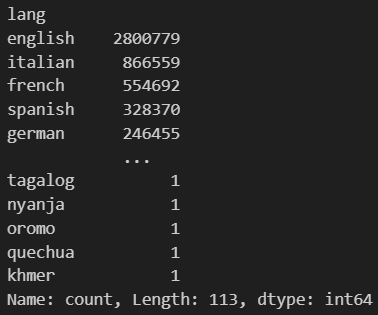
\includegraphics[width=0.5\textwidth]{Images/cld2.png}}
    \captionsetup{font=footnotesize}
    \caption{\textit{Compact Language Detector 2 Results. Source: Author’s own elaboration based on Inside Airbnb}}
    \label{fig:cld2}
\end{figure}

\indent The remaining reviews were tokenised using the \texttt{word\_tokenize} function from the \texttt{NLTK} library. All tokens were converted to lowercase to maintain consistency and reduce redundancy caused by case differences. Stopwords and punctuation marks were then removed using the NLTK English stopword list and the \texttt{string} library, respectively. A custom cleaning function was applied to remove both types of noise, leaving only meaningful tokens. Subsequently, all words were lemmatised using the \texttt{spaCy} library to reduce them to their base or dictionary form (e.g., “running” $\rightarrow$ “run”). To optimise performance, texts were processed in batches of 2,000 using parallelisation across four cores. The cleaned and lemmatised tokens were then stored as a new variable in the dataset, producing a standardised textual representation suitable for further computational analysis, such as topic modelling and sentiment classification.

\begin{algorithm}[ht]
\caption{Lemmatizing Reviews}\label{alg:lemmatize_reviews}
\begin{algorithmic}[1]
\Require Data frame $airbnb\_reviews\_sample$ with column \texttt{clean\_tokens}
\State Initialize empty list $lemma\_token\_list \gets [\,]$
\State Create list $texts \gets$ join tokens in each element of $airbnb\_reviews\_sample[\texttt{clean\_tokens}]$ with spaces
\For{each $doc$ in NLP pipeline applied to $texts$ with batch size $2000$ and $n\_process = 4$}
    \State Extract $lemmas \gets$ list of $token.lemma\_$ for each $token$ in $doc$
    \State Exclude tokens that are punctuation or spaces
    \State Append $lemmas$ to $lemma\_token\_list$
\EndFor
\Ensure List $lemma\_token\_list$ containing lemmatized tokens for each review
\end{algorithmic}
\end{algorithm}

\indent Following this text preprocessing, the cleaned tokens were converted into numerical features using the TF–IDF method, as described before. Both unigrams (single words) and trigrams (three-word sequences) were extracted using the following pseudocode:

\begin{algorithm}[ht]
\caption{Computing TF-IDF Vectors}\label{alg:compute_tfidf_vectors}
\begin{algorithmic}[1]
\Require List of documents $doc$ \\
\Comment{--- Compute TF-IDF for unigrams ---}
\State Initialize \texttt{vectorizer\_unigrams} $\gets$ \texttt{TfidfVectorizer} with parameters:
\begin{itemize}
    \item \texttt{lowercase = False}
    \item \verb|token_pattern = r"(?u)\b\w+\b"|
    \item \texttt{ngram\_range = (1,1)}
    \item \texttt{min\_df = 5}, \texttt{max\_df = 0.8}
    \item \texttt{max\_features = 100{,}000}
    \item \texttt{dtype = float32}
\end{itemize}
\State Fit and transform $doc$ using \texttt{vectorizer\_unigrams} to obtain matrix $X\_{unigrams}$
\State Extract feature names $terms\_{unigrams} \gets$ \texttt{vectorizer\_unigrams.get\_feature\_names\_out()} \\
\Comment{--- Compute TF-IDF for trigrams ---}
\State Initialize \texttt{vectorizer\_trigrams} $\gets$ same parameters as above, but with \texttt{ngram\_range = (3,3)}
\State Fit and transform $doc$ using \texttt{vectorizer\_trigrams} to obtain matrix $X\_{trigrams}$
\State Extract feature names $terms\_{trigrams} \gets$ \texttt{vectorizer\_trigrams.get\_feature\_names\_out()}
\Ensure TF-IDF matrices $X\_{unigrams}$ and $X\_{trigrams}$, and their corresponding term lists
\end{algorithmic}
\end{algorithm}


\indent The TF–IDF scores were aggregated across all documents to obtain a global measure of each term’s relative importance. To visualise the most relevant words in the corpus, a word cloud was generated using the \texttt{WordCloud} library, where word size corresponds to cumulative TF–IDF scores. Additionally, the top 20 terms were identified and presented in tabular form, ranked by their total TF–IDF weight.

\indent The other dataset used in this work is the Booking.com Reviews Dataset, which is a comprehensive collection of hotel reviews and ratings gathered from the popular travel booking platform, Booking.com. This dataset provides valuable insights into customers’ experiences and perceptions of hotels across various destinations \cite{bookingdata}. After importing the dataset, reviews containing the text “There are no comments available for this review” were removed, leaving a total of 18,988 valid records for analysis.  

\indent Each review was tokenised using the \texttt{word\_tokenize} function from the \texttt{NLTK} library, and all tokens were converted to lowercase to ensure consistency. As in the Airbnb pipeline, stopwords (from NLTK’s English stopword list) and punctuation marks (from Python’s \texttt{string} library) were removed to retain only semantically meaningful words. The resulting tokens were then lemmatised as done with the previous dataset, using Algorithm~\ref{alg:lemmatize_reviews}. A final cleaning step was applied to remove generic or low-information terms such as “review” and “comment.”

\indent After preprocessing, the dataset was divided into two subsets based on the rating score:

\begin{itemize}
    \item Positive reviews: ratings $\geq 7$
    \item Negative reviews: ratings $< 7$
\end{itemize}

\indent For each subset (positive and negative), a TF–IDF vectoriser was applied to transform the lemmatised text into a numerical representation, following the same steps as done with Aribnb's dataset (Algorithm~\ref{alg:compute_tfidf_vectors}). The resulting TF–IDF matrices were aggregated to identify the most relevant terms within positive and negative reviews. To visualise these patterns, word clouds were generated, with word size proportional to cumulative TF–IDF scores. Additionally, the top 20 terms were extracted and presented in tabular form for each subset, offering a clear comparison of the dominant lexical features that distinguish positive and negative customer experiences.

\subsection{Results}

\indent After applying the TF–IDF method to the Airbnb dataset, the unigram analysis revealed that the most frequent terms were primarily related to the location of the property and the services offered by the accommodation. This suggests that, when writing reviews, guests tend to emphasise not only the geographical setting (e.g., location, walk, or close) but also the specific amenities provided (e.g., clean, comfortable, or amenity). As shown in Figure~\ref{fig:airbnbunigram} (see Appendix~\ref{sec:airbnbwords}), these two dimensions—location and services—emerged as dominant topics shaping guests’ perceptions and experiences.

\indent To gain a more detailed understanding, the same analysis was conducted using trigrams. As shown in Figure~\ref{fig:airbnbtrigram}, the results further reinforced the centrality of location, with frequent expressions such as “place great location”, “great location close”, “within walking distance”, and “close train station”. In contrast, there were relatively few trigrams directly associated with services, and several of the most frequent ones still referred to location, such as “clean great location”. This indicates that, even when considering multi-word expressions, guests consistently prioritise aspects related to the property’s location over other features of the accommodation.

\begin{figure}[ht]
    \centering
    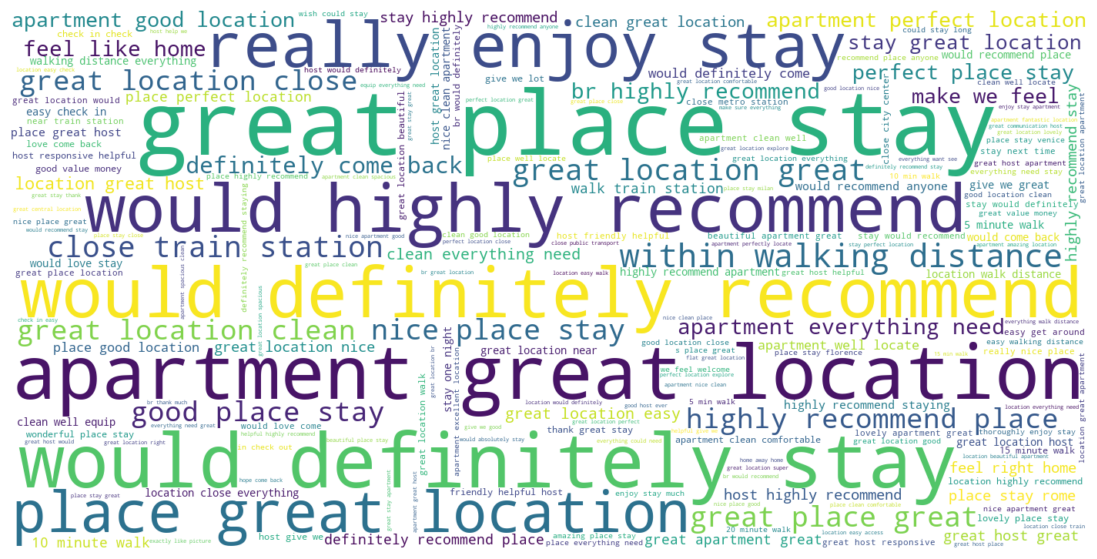
\includegraphics[width=0.9\textwidth]{Analysis/Airbnb 3-gram.png}
    \captionsetup{font=footnotesize}
    \caption{\textit{Airbnb Reviews' Top 3-grams. Source: Author’s own elaboration based on Inside Airbnb}}
    \label{fig:airbnbtrigram}
\end{figure}

\indent Turning to the Booking.com dataset, the unigram analysis of positive reviews revealed that the most frequent terms were again related to both the location of the property and the services provided by the accommodation. As shown in Figure~\ref{fig:bookingpword} (see Appendix~\ref{sec:bookingtopwords}), compared with the Airbnb reviews, a greater number of terms referred to specific services such as “breakfast”, “reception”, “garden”, and “bed”. In addition, new location-related terms appeared, including “metro” and “restaurant”.

\indent In contrast, the unigram analysis of negative reviews (see Figure~\ref{fig:bookingnword} in Appendix~\ref{sec:bookingtopwords}) showed that, although “location” remained a highly frequent term, a larger share of the most common words referred to accommodation services, including “shower”, “bathroom”, “bed”, and “staff”.

\indent The trigram analysis of positive reviews (see Figure~\ref{fig:bookingptri}) highlighted the growing importance of accommodation services, with common expressions such as “friendly helpful staff” and “room comfortable bed”. Location, however, remained a crucial factor, with trigrams such as “within walking distance” and “close city center”.

\begin{figure}[ht]
    \centering
    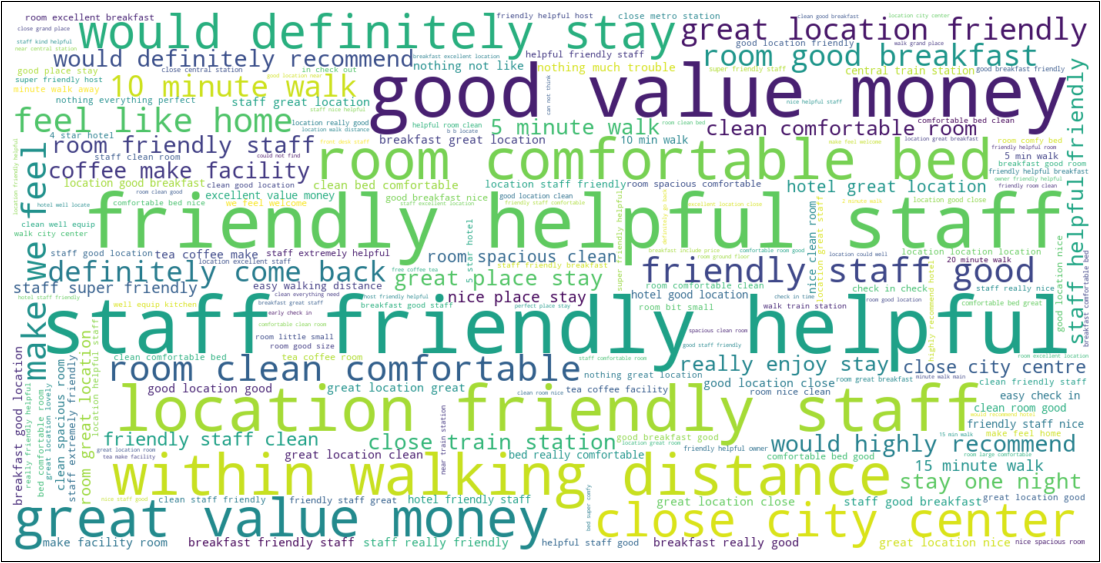
\includegraphics[width=0.9\textwidth]{Analysis/Booking Positive Scores 3-Gram.png}
    \captionsetup{font=footnotesize}
    \caption{\textit{Booking.com Positive Reviews' 3-grams. Source: Author’s own elaboration based on a Kaggle's dataset}}
    \label{fig:bookingptri}
\end{figure}

\indent As shown in Figure~\ref{fig:bookingntri}, the trigram analysis of negative reviews revealed a stronger emphasis on location, with expressions such as “close train station”, “5 minute walk”, and “close city center”. At the same time, several trigrams provided clearer insights into service-related concerns, including “4 star hotel”, “friendly helpful staff”, and “coffee make facility”.

\begin{figure}[ht]
    \centering
    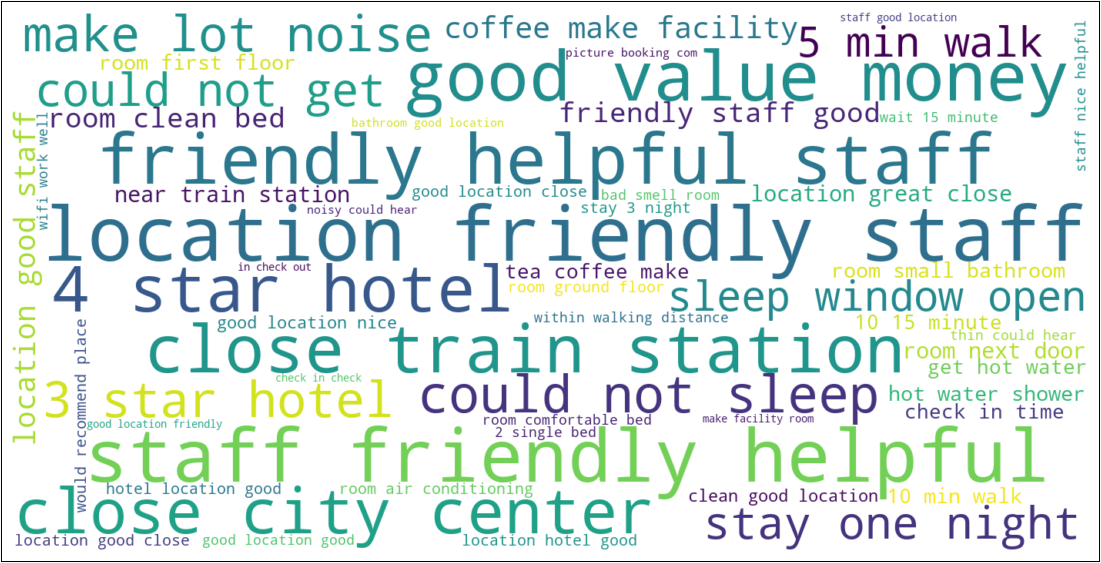
\includegraphics[width=0.9\textwidth]{Analysis/Booking Negative Scores 3-gram.png}
    \captionsetup{font=footnotesize}
    \caption{\textit{Booking.com Negative Reviews' 3-grams. Source: Author’s own elaboration based on a Kaggle's dataset.}}
    \label{fig:bookingntri}
\end{figure}

\indent Based on the insights obtained from the textual analyses of both datasets, the list of attributes was refined and improved as follows:

\begin{figure}[ht]
    \centering
    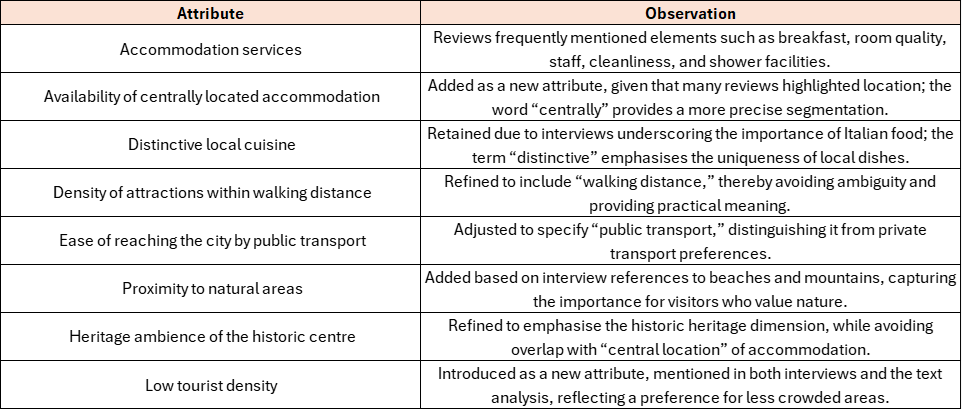
\includegraphics[width=1\textwidth]{Images/Accommodation Reviews/reviews_att.png}
    \captionsetup{font=footnotesize}
    \caption{\textit{Refined Set of 10 Preliminary Attributes. Source: Author’s own elaboration.}}
    \label{fig:reviews_att}
\end{figure}


\section{Explanatory Survey}

\subsection{Methodology}

\indent To further advance the analysis, an explanatory survey (see Appendix~\ref{sec:explanatorysurvey}) was conducted using Microsoft Forms to capture travelers’ perceptions, decision-making processes, and experiences related to tourism. The survey was available in both English and Spanish and distributed to 25 respondents without disclosing the specific research purpose. Data collection concluded once all 25 responses had been received. This stage functioned as a bridge between the qualitative interviews and the final quantitative survey, serving both to test question clarity and to generate additional insights for refining the set of destination attributes.

\indent The survey combined open-ended and structured questions. The open-ended questions invited respondents to narrate personal travel experiences (e.g., unsatisfactory trips, representative vacations, or memorable journeys) and to offer advice to their “past self” regarding travel decision-making. Scenario-based questions (scene choices) were also included to explore how travelers evaluate different destination settings. The structured questions focused on decision-making steps, missing factors in information searches, levels of information saturation, and perceptions of pricing. For the latter, a question based on Van Westendorp’s Price Sensitivity Meter was included to estimate acceptable price ranges for a tourism package. This model offers a comprehensive multi-question framework that indirectly measures willingness to pay, identifying a range of acceptable prices rather than a single point estimate \cite{vanwestern}.

\indent Once collected, responses in Spanish were translated into English using ChatGPT, followed by careful manual verification to ensure accuracy. The dataset was then imported into Google Colab for processing, where column names were standardised. An exploratory data analysis (EDA) was conducted to summarise key statistics and visualise general respondent characteristics. For the Van Westendorp model, inconsistent responses, such as cases in which the “too cheap” value exceeded the “bargain” value, were removed. Outliers were excluded using the interquartile range thresholds (\texttt{Q1 - 1.5 × IQR} and \texttt{Q3 + 1.5 × IQR}). This procedure enabled the estimation of price thresholds for “too cheap,” “bargain,” “expensive,” and “too expensive,” ultimately identifying the Optimal Price Point (OPP), by implementing the Algorithm~\ref{alg:vw_code} (see Appendix~\ref{sec:vwcode}).

\indent The textual responses were processed using a standardised natural language preprocessing pipeline, which included:

\begin{itemize}
    \item Conversion of text to lowercase.
    \item Removal of punctuation, special characters, and extra spaces.
    \item Normalisation of accented characters.
    \item Tokenisation and lemmatisation using \texttt{spaCy}.
    \item Stopword removal to retain only meaningful terms.
\end{itemize}

\indent The analysis followed a text-mining approach combining both a semantic and frequency-based techniques. Sentence embeddings (using \texttt{SentenceTransformers}) were employed to capture semantic similarity and group related responses, with cosine similarity calculated through the \texttt{networkx} library. TF–IDF vectorisation was subsequently applied within each semantic cluster to identify the most frequent words and expressions. Sentence embeddings were first used to group responses, followed by TF–IDF analysis within each group, for the following open-ended questions:

\begin{itemize}
\item “Tell us about a trip of yours that you were not satisfied with. What would you not do again, especially in the planning phase?” (similarity fixed greater than 0.7).
\item “Which trip or vacation best represents your way of choosing how to travel? Tell us about the destination: how you chose it, why it reflects you, etc” (similarity fixed greater than 0.67).
\item “If you had to teach someone your method of choosing, which 3 fundamental steps would you tell them to follow?” (similarity fixed greater than 0.7).
\item “If instead you had to give 3 pieces of advice to your past self about organising a vacation, what would you say?” (similarity fixed greater than 0.7).
\item “When you organised your last vacation, did you have a list of destinations in mind? How did you make your final choice? And among them, was there a destination you said, ‘No, this is not for me’?” (similarity fixed greater than 0.7).
\end{itemize}

\indent For other questions, only TF–IDF vectorisation was applied, using different n-gram configurations depending on the length and structure of responses:

\begin{itemize}
\item “Imagine organising a vacation. Sketch a short story of your choice: what would be the 3–4 main scenes?”
\item “Which was the decisive piece of information you looked at last before choosing?”
\item “When did you feel you had ‘enough’ information to decide? What made you stop searching? And if you had had more time, what would you have added to your research?”
\item “What type of trip do you usually choose: a short trip, a medium-length trip, or a long one? Please explain the reason for your choice.”
\end{itemize}

\indent In some cases, additional steps were taken prior to text analysis. For the question “Which was the decisive piece of information you looked at last before choosing?”, responses were divided into two groups (A and B) according to the answer to the preceding question, “If you had to choose right now, which of the two screens would you pick?”. For the question “What type of trip do you usually choose: a short trip, a medium-length trip, or a long one? Please explain the reason for your choice”, responses were manually labelled based on the preferred trip length (short, medium, long, or not defined). Finally, for the questions “If you had to teach someone your method of choosing, which 3 fundamental steps would you tell them to follow?” and “If instead you had to give 3 pieces of advice to your past self about organising a vacation, what would you say?”, all steps were concatenated for each case, preserving their order, so that each respondent’s full set of steps or pieces of advice could be analysed as a single continuous text.

\indent Finally, using the same prompt described previously (see Appendix~\ref{sec:chatgpt_prompts}), the raw dataset containing all responses was uploaded to ChatGPT. The model was asked to examine each column carefully and extract any tourist-related attributes identified within the answers. In addition, a series of personal observations and comparative notes were made to evaluate how ChatGPT’s results aligned with the attributes previously obtained from the text mining processand to determine whether any new attributes emerged from its output. This step allowed for a cross-validation between human interpretation and AI-assisted analysis.

\subsection{Results}

\subsection{Exploratory Data Analysis (EDA)}

\indent The exploratory analysis of the explanatory survey dataset provided a general profile of the average respondent (see Figures~\ref{fig:descriptivedata} and~\ref{fig:descriptivedata2} in Appendix~\ref{sec:expsurvresults} for additional visualisations). The results suggest that most participants were young adults between 25 and 35 years old, although a secondary group of respondents aged over 60 was also identified. The majority of respondents were female and employed, with South America representing the most common region of origin. In terms of travel behaviour, participants typically organised trips collaboratively and tended to travel with companions such as partners, family, or friends. As shown in Figure~\ref{fig:descriptivemain}, the primary motivation for travel was exploring new cities, although relaxation was also cited as a complementary purpose.

\begin{figure}[ht]
    \centering
    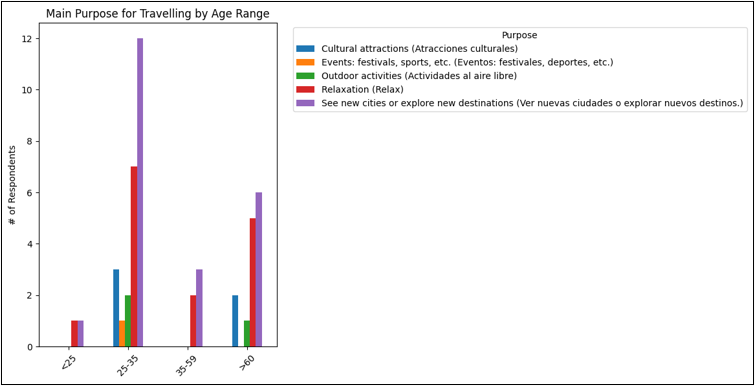
\includegraphics[width=0.9\textwidth]{Images/Explanatory Survey/Descriptive_main.png}
    \captionsetup{font=footnotesize}
    \captionof{figure}{\textit{Main Purpose for Travelling. Source: Author’s own elaboration based on survey data.}}
    \label{fig:descriptivemain}
\end{figure}

\indent Notable differences emerged across age groups: younger respondents reported relying primarily on Google or similar platforms—and in some cases ChatGPT—for information searches, whereas older respondents showed a stronger reliance on travel blogs or agencies. Regarding decision-making patterns, respondents generally reported considering three to four destination options and taking several days to evaluate alternatives before confirming their booking, as shown in Figure~\ref{fig:descriptivemain2}.

\begin{figure}[ht]
    \centering
    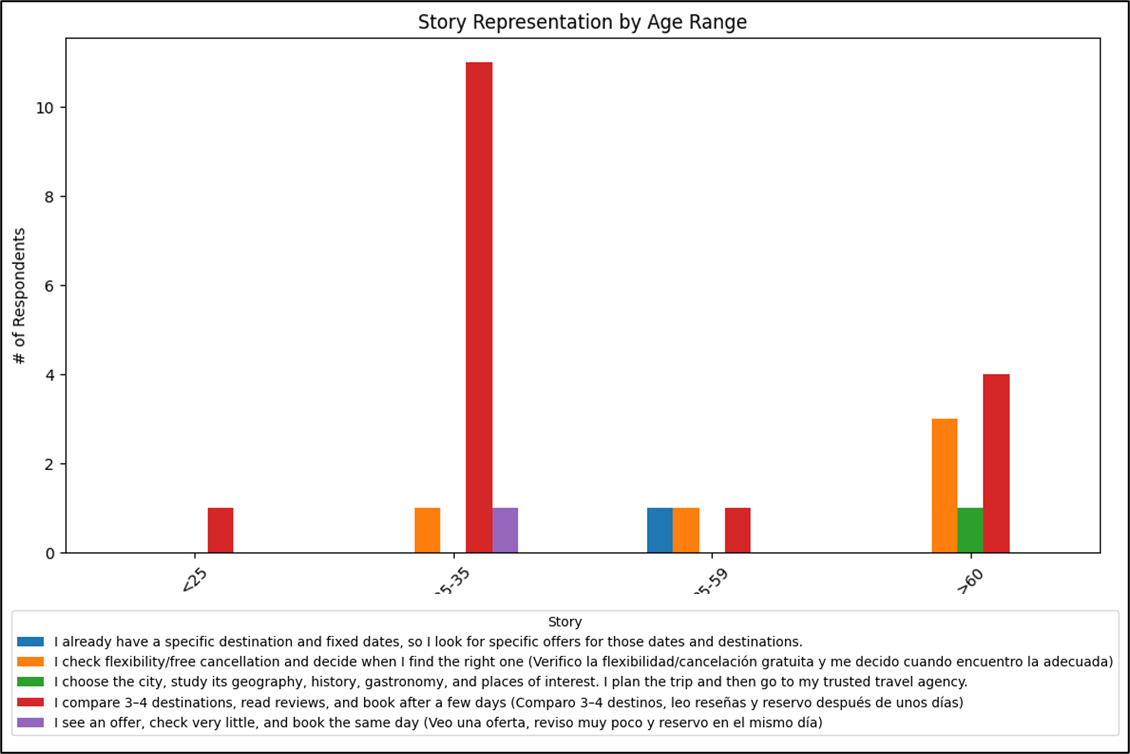
\includegraphics[width=0.9\textwidth]{Images/Explanatory Survey/Descriptive_main2.png}
    \captionsetup{font=footnotesize}
    \captionof{figure}{\textit{Description of Explanatory Survey's Respondents. Source: Author’s own elaboration based on survey data.}}
    \label{fig:descriptivemain2}
\end{figure}

\subsection{Van Westendorp Price Sensitivity Analysis}

\indent The analysis of price perceptions using the Van Westendorp method revealed notable differences across age groups. For the full sample (see Figure~\ref{fig:vwfull}), after removing outliers and inconsistent responses, the Optimal Price Point (OPP) was estimated at €250.06. When the analysis was segmented, clear differences emerged: respondents aged 35 or younger reported a substantially lower OPP of €150.20 (see Figure~\ref{fig:vwage} in Appendix~\ref{sec:vanwestendorp}), whereas those older than 35 years displayed a much higher OPP of €279.46 (see Figure~\ref{fig:vwage} in Appendix~\ref{sec:vanwestendorp}). For the latter group, outliers were retained, as their removal resulted in no definable OPP. These findings indicate that younger respondents demonstrate greater price sensitivity and a lower willingness to pay for tourism products, whereas older respondents are generally more willing to spend, suggesting distinct consumer profiles relevant for market segmentation and pricing strategies.

\begin{figure}[ht]
    \centering
    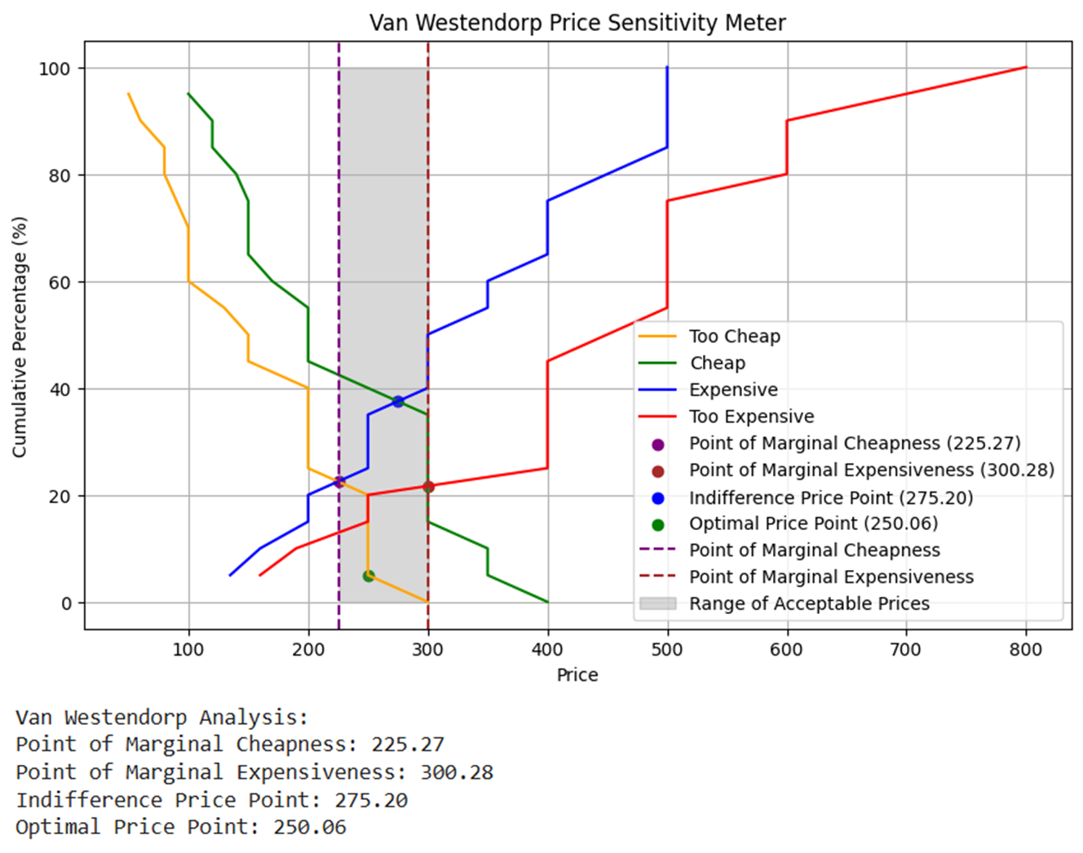
\includegraphics[width=0.9\textwidth]{Images/Explanatory Survey/Van Westendorp.png}
    \captionsetup{font=footnotesize}
    \captionof{figure}{\textit{Van Westendorp Pricing Method with Full Sample. Source: Author’s own elaboration based on survey data.}}
    \label{fig:vwfull}
\end{figure}

\subsection{Text Mining, Embeddings \& TF-IDF}

\subsubsection{Unsatisfying Trip}

\indent In response to the question “Tell us about a trip of yours that you were not satisfied with. What would you not do again, especially in the planning phase?”, two groups were identified. The first group (see Figure~\ref{fig:worst1}), composed mainly of young adults (25–35), emphasised poor organisation as the main reason for dissatisfaction.

\begin{figure}[ht]
    \centering
    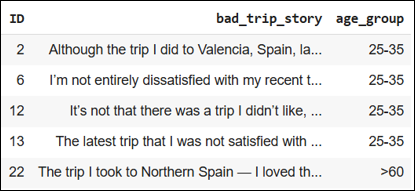
\includegraphics[width=0.5\textwidth]{Images/Explanatory Survey/Worst Trip - Group 1.png}
    \captionsetup{font=footnotesize}
    \captionof{figure}{\textit{Unsatisfying Trip - Group 1. Source: Author’s own elaboration based on survey data.}}
    \label{fig:worst1}
\end{figure}

\indent The second group (see Figure~\ref{fig:worst2}) comprised respondents aged over 60, who mainly attributed their unsatisfactory experience to not booking tours conducted in their native language.

\begin{figure}[ht]
    \centering
    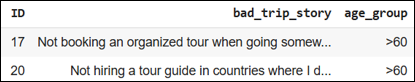
\includegraphics[width=0.5\textwidth]{Images/Explanatory Survey/Worst Trip - Group 2.png}
    \captionsetup{font=footnotesize}
    \captionof{figure}{\textit{Unsatisfying Trip - Group 2. Source: Author’s own elaboration based on survey data.}}
    \label{fig:worst2}
\end{figure}

\subsubsection{Satisfying Trip}

\indent For the question “Which trip or vacation best represents your way of choosing how to travel? Tell us about the destination: how you chose it, why it reflects you, etc.”, two groups were also identified. The first group (see Figure~\ref{fig:best1}) included both young adults (25–35) and older participants (>60). These respondents typically described trips in which they visited multiple destinations, most often in Europe, a continent that enables visiting several cities within a single trip.

\begin{figure}[ht]
    \centering
    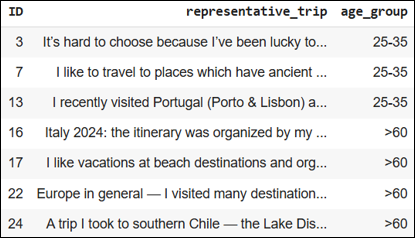
\includegraphics[width=0.5\textwidth]{Images/Explanatory Survey/Best Trip - Group 1.png}
    \captionsetup{font=footnotesize}
    \captionof{figure}{\textit{Satisfying Trip - Group 1. Source: Author’s own elaboration based on survey data.}}
    \label{fig:best1}
\end{figure}

\indent The second group (see Figure~\ref{fig:best2}) comprised two respondents, both young adults, who expressed a preference for visiting multiple destinations, including cruises, while highlighting the importance of relaxation as a core element of their ideal trip.

\begin{figure}[ht]
    \centering
    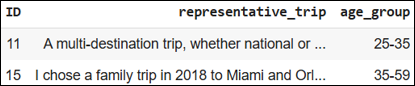
\includegraphics[width=0.5\textwidth]{Images/Explanatory Survey/Best Trip - Group 2.png}
    \captionsetup{font=footnotesize}
    \captionof{figure}{\textit{Satisfying Trip - Group 2. Source: Author’s own elaboration based on survey data.}}
    \label{fig:best2}
\end{figure}

\subsubsection{Organizing a Vacation}

\indent In the question “Imagine organising a vacation. Sketch a short story of your choice: what would be the 3–4 main scenes?”, each step was analysed separately using TF–IDF vectorisation. In the first stage, respondents primarily focused on defining the destination, often new or unexplored places, and aligning it with their available budget (see Figure~\ref{fig:organizing1}).

\begin{figure}[ht]
    \centering
    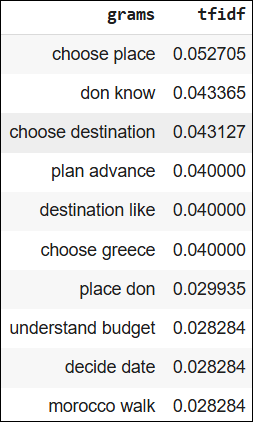
\includegraphics[width=0.2\textwidth]{Images/Explanatory Survey/Organizing (step 1).png}
    \captionsetup{font=footnotesize}
    \captionof{figure}{\textit{Organizing a Vacation - Step 1. Source: Author’s own elaboration based on survey data.}}
    \label{fig:organizing1}
\end{figure}

\indent The second stage (see Figure~\ref{fig:organizing2}) was mainly described by planning logistics, such as defining travel dates, purchasing plane tickets, booking accommodation, and comparing different options.

\begin{figure}[ht]
    \centering
    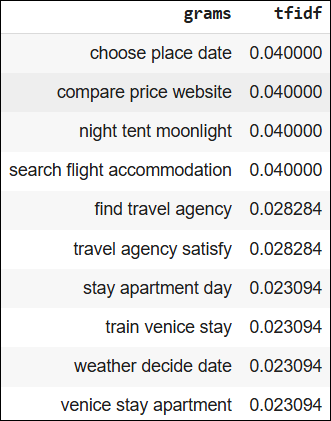
\includegraphics[width=0.3\textwidth]{Images/Explanatory Survey/Organizing (step 2).png}
    \captionsetup{font=footnotesize}
    \captionof{figure}{\textit{Organizing a Vacation - Step 2. Source: Author’s own elaboration based on survey data.}}
    \label{fig:organizing2}
\end{figure}

\indent The third stage focused mainly on defining the itinerary and selecting activities at the destination (see Figure~\ref{fig:organizing3}). The optional fourth stage (see Figure~\ref{fig:organizing4}) often repeated previous elements, such as defining accommodation or activities, confirming their importance in the final stages of trip planning.

\begin{figure}[ht]
    \centering
    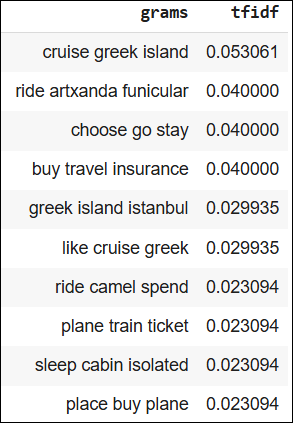
\includegraphics[width=0.3\textwidth]{Images/Explanatory Survey/Organizing (step 3).png}
    \captionsetup{font=footnotesize}
    \captionof{figure}{\textit{Organizing a Vacation - Step 3. Source: Author’s own elaboration based on survey data.}}
    \label{fig:organizing3}
\end{figure}

\begin{figure}[ht]
    \centering
    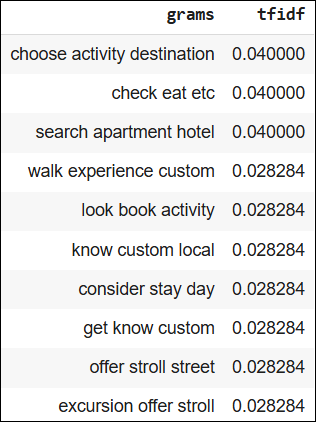
\includegraphics[width=0.3\textwidth]{Images/Explanatory Survey/Organizing (step 4).png}
    \captionsetup{font=footnotesize}
    \captionof{figure}{\textit{Organizing a Vacation - Step 4. Source: Author’s own elaboration based on survey data.}}
    \label{fig:organizing4}
\end{figure}

\subsubsection{Choosing Between Two options}

\indent Most participants (72\%) preferred option B, primarily due to the possibility of free cancellation. Some also mentioned reviews as a secondary factor. Conversely, those who chose option A (28\%) mainly cited price as the decisive factor. Figure~\ref{fig:screenchoose} displays the most frequent bigrams for each group.

\begin{figure}[ht]
    \centering
    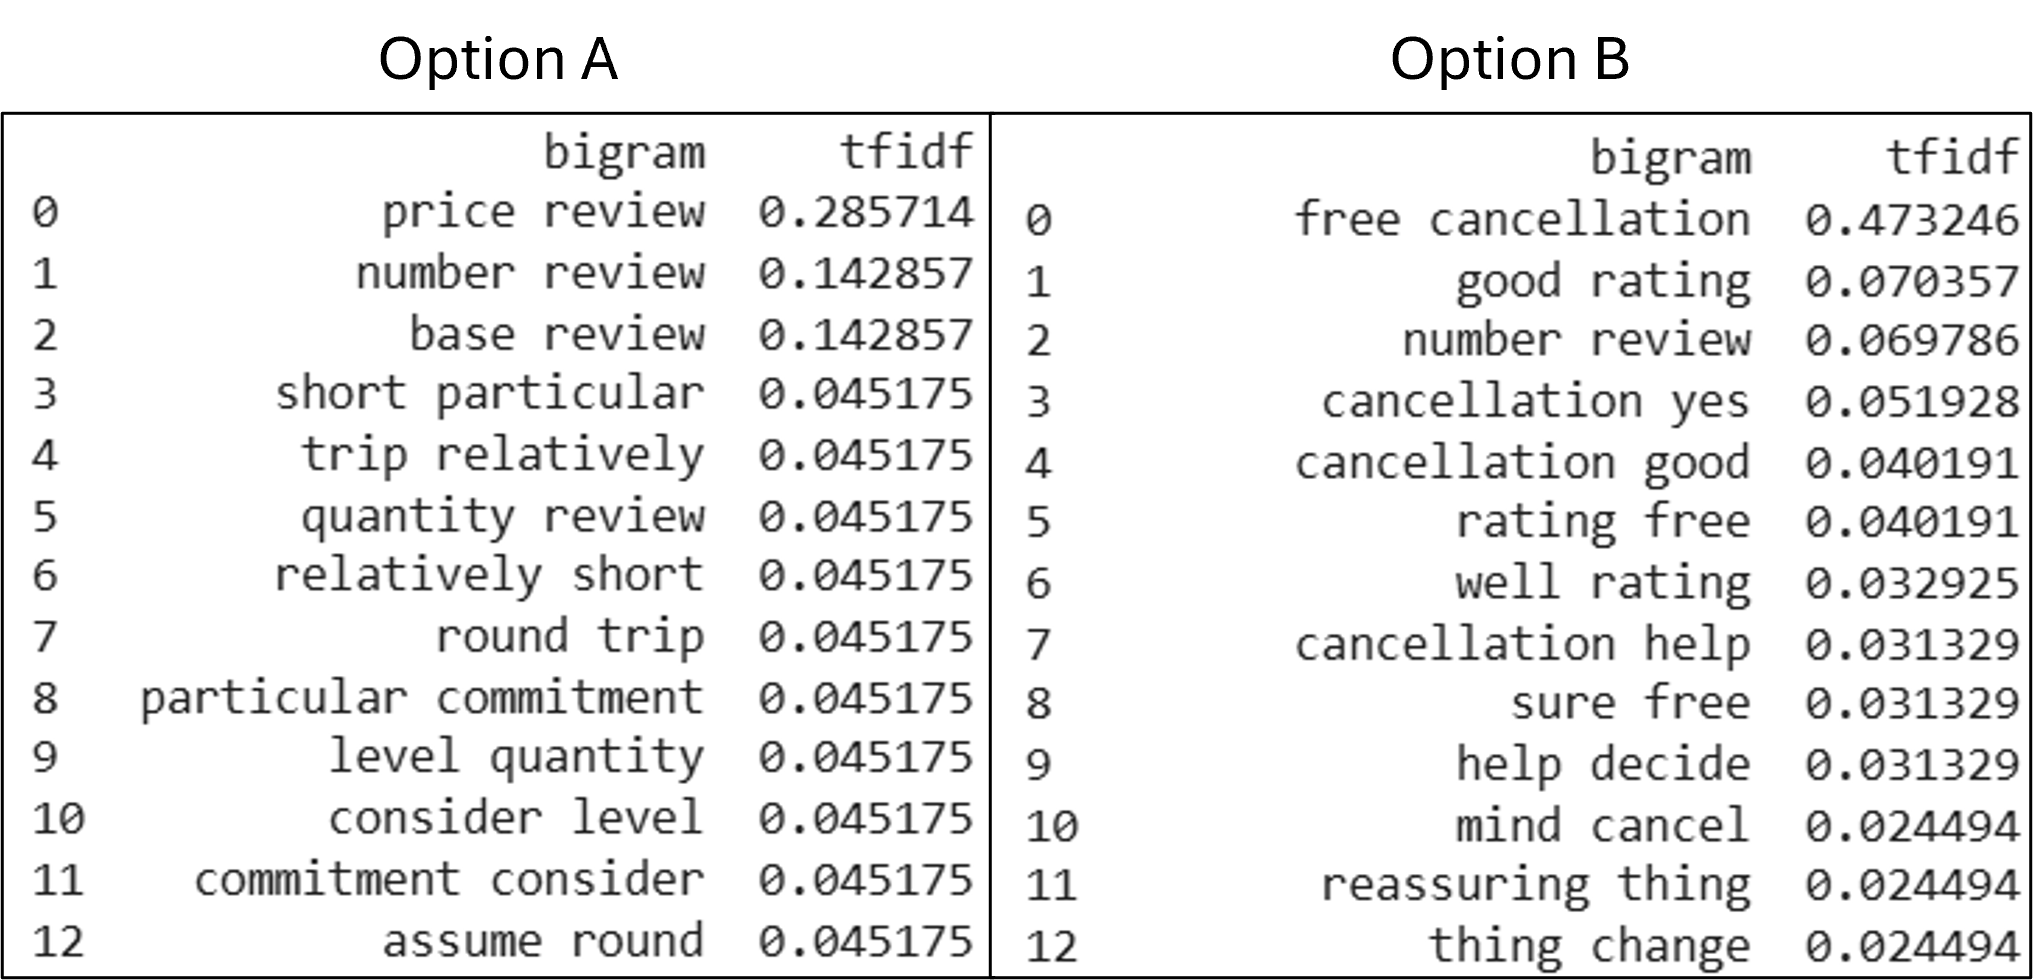
\includegraphics[width=0.8\textwidth]{Images/Explanatory Survey/Screen Choose.png}
    \captionsetup{font=footnotesize}
    \captionof{figure}{\textit{Group A and B. Source: Author’s own elaboration based on survey data.}}
    \label{fig:screenchoose}
\end{figure}

\subsubsection{Choosing Method}

\indent The embedding similarity analysis for the question “If you had to teach someone your method of choosing, which 3 fundamental steps would you tell them to follow?” yielded a single cluster containing 11 responses (see Figure~\ref{fig:choosingmethod}). This group comprised mainly young adults (25–35) and a smaller proportion of older respondents (>60). Both embedding similarity and TF–IDF analyses highlighted a consistent decision-making pattern: beyond defining the destination, respondents placed strong emphasis on checking recommendations, verifying accommodation availability, and planning the trip in advance.

\begin{figure}[ht]
    \centering
    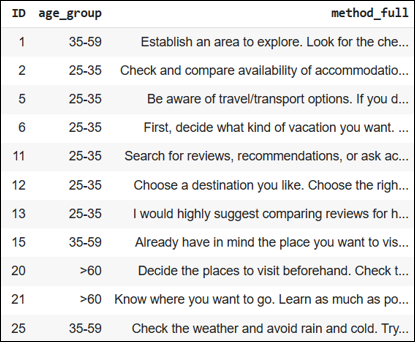
\includegraphics[width=0.5\textwidth]{Images/Explanatory Survey/Method of Choosing.png}
    \captionsetup{font=footnotesize}
    \captionof{figure}{\textit{Choosing Method Group. Source: Author’s own elaboration based on survey data.}}
    \label{fig:choosingmethod}
\end{figure}

\indent Based on these insights, the decision-making process for this group can be summarised in three steps:

\begin{enumerate}
    \item Define \& Learn: Decide on the type of trip and preferred destination, and gather initial information about the location.
    \item Check \& Compare: Review recommendations, compare accommodation and transport options, and verify availability.
    \item Plan \& Book: Create a detailed plan, book accommodations and key activities in advance, and prepare financially.
\end{enumerate}

\subsubsection{Advice to Their ``Past Self''}

\indent For the question “If instead you had to give 3 pieces of advice to your past self about organising a vacation, what would you say?”, two groups were identified. The first (see Figure~\ref{fig:past_self}) included a majority of older participants (>60) but also a considerable number of young adults (25–35).

\begin{figure}[ht]
    \centering
    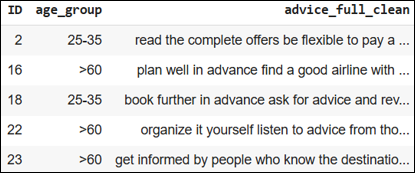
\includegraphics[width=0.5\textwidth]{Images/Explanatory Survey/Advice (Group 1).png}
    \captionsetup{font=footnotesize}
    \captionof{figure}{\textit{Advice to ``Past Self'' - Group 1. Source: Author’s own elaboration based on survey data.}}
    \label{fig:past_self}
\end{figure}

\indent The main themes extracted were as follows:

\begin{itemize}
    \item Good preparation:
    \begin{itemize}
        \item Read offers carefully and understand what is included.
        \item Plan and book early, especially for flights and hotels.
        \item Get informed from reliable sources, such as experienced travelers, review sites, and travel forums.
    \end{itemize}
    \item Choose Carefully:
    \begin{itemize}
        \item Quality and reliability matter.
        \item Choose hotels with at least 3 stars or good reviews.
        \item Select transfers carefully.
    \end{itemize}
    \item Spend Smart:
    \begin{itemize}
        \item Be willing to pay a bit more for better quality and comfort.
        \item Balance between booking in advance and leaving room for spontaneous activities.
    \end{itemize}
\end{itemize}

\indent The second group (see Figure~\ref{fig:past_self2}) consisted primarily of young adults (25–35), along with a few older respondents (>60). The main pieces of advice identified from this group were:

\begin{itemize}
    \item Plan with time but leave some room for spontaneous experiences.
    \item Take your time to compare options.
    \item Book tours to get to know better the city.
    \item Check transportation.
\end{itemize}

\begin{figure}[ht]
    \centering
    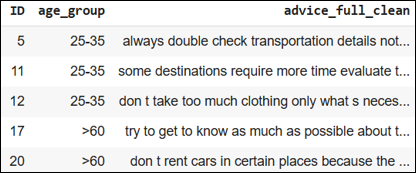
\includegraphics[width=0.5\textwidth]{Images/Explanatory Survey/Advice (Group 2).png}
    \captionsetup{font=footnotesize}
    \captionof{figure}{\textit{Advice to ``Past Self'' - Group 2. Source: Author’s own elaboration based on survey data.}}
    \label{fig:past_self2}
\end{figure}

\subsubsection{Defining the Destination}

\indent The question “When you organised your last vacation, did you have a list of destinations in mind? How did you make your final choice?” produced two groups. The first (see Figure~\ref{fig:definition1}) comprised mainly young adults (25–35) and a few older participants (>60). Most respondents began with a list of potential destinations, narrowing it down based on preferences such as activities, local events, and desired experiences. Some excluded destinations considered overly touristic, while a few made spontaneous choices without a predefined list, balancing planning with flexibility.

\begin{figure}[ht]
    \centering
    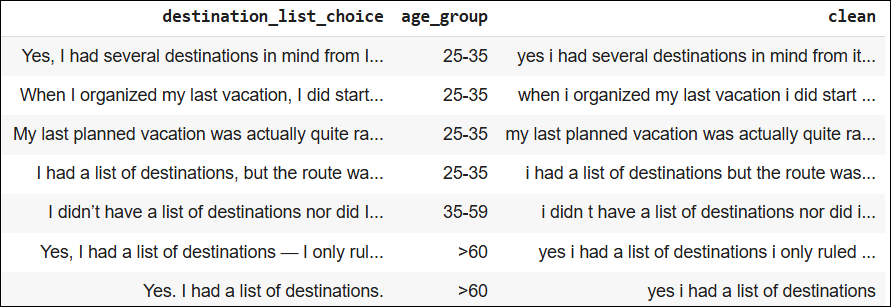
\includegraphics[width=0.8\textwidth]{Images/Explanatory Survey/Definition (Group 1).png}
    \captionsetup{font=footnotesize}
    \captionof{figure}{\textit{Defining the Destination - Group 1. Source: Author’s own elaboration based on survey data.}}
    \label{fig:definition1}
\end{figure}

\indent The second group (see Figure~\ref{fig:definition2}) included only young adults. Their responses focused strongly on practical factors such as cost and time availability, indicating decisions guided more by feasibility and affordability than by emotional preference.

\begin{figure}[ht]
    \centering
    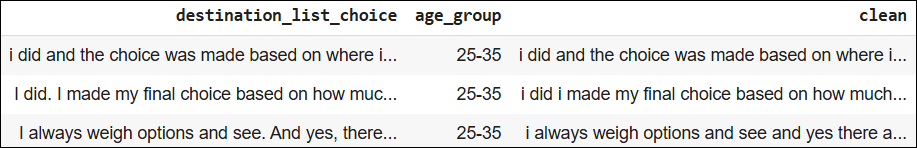
\includegraphics[width=0.8\textwidth]{Images/Explanatory Survey/Definition (Group 2).png}
    \captionsetup{font=footnotesize}
    \captionof{figure}{\textit{Defining the Destination - Group 2. Source: Author’s own elaboration based on survey data.}}
    \label{fig:definition2}
\end{figure}

\subsubsection{Information Saturation}

\indent As shown in Figure~\ref{fig:infosaturation}, most participants reported stopping their search once they had gathered essential information, such as dates, accommodation, transport, and prices, that made them feel confident in their decision. Avoiding information overload was a key trigger to stop searching. For example, one respondent noted that social media can sometimes create unnecessary information overload, promoting distrust rather than clarity. If given more time, some respondents indicated they would have explored nearby destinations, searched for better deals, or extended their stay, while a few felt no need to add anything further.

\begin{figure}[ht]
    \centering
    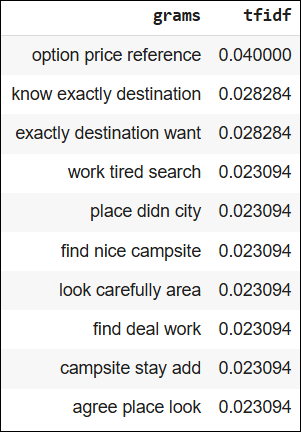
\includegraphics[width=0.3\textwidth]{Images/Explanatory Survey/Info Saturation.png}
    \captionsetup{font=footnotesize}
    \captionof{figure}{\textit{Top Trigrams for Information Saturation. Source: Author’s own elaboration based on survey data.}}
    \label{fig:infosaturation}
\end{figure}

\subsection{Additional Observations}

\indent Combined with the results presented above, responses to the question “Is there something important we haven’t asked you but that influenced your decision? Tell us about it.” provided additional insights for attribute refinement. Although few participants provided responses, some noteworthy comments included:

\begin{itemize}
    \item ``...the opportunity to learn something new. Whether it’s history, local traditions, or even trying a completely new activity.''
    \item ``Ticket prices and promotions always influence my decision.''
    \item ``I listen to other travelers’ stories and take what might interest me.''
\end{itemize}

\subsubsection{Complementary Attribute Discovery through ChatGPT}

\indent Regarding the suggestions from ChatGPT, as shown in Figure~\ref{fig:expsurvchat}, although most of the attributes were related to existing ones, there was one attribute that consistently appeared across the analyses and suggestions: Availability of guided tours in different languages.

\begin{figure}[ht]
    \centering
    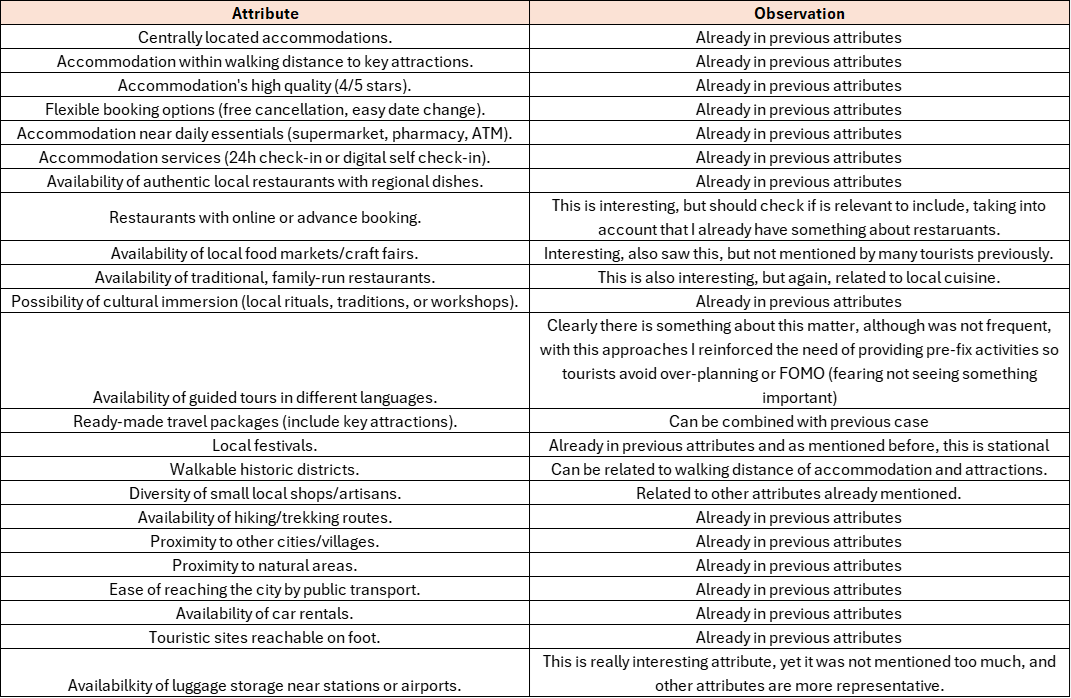
\includegraphics[width=1\textwidth]{Images/Explanatory Survey/ChatGPT.png}
    \captionsetup{font=footnotesize}
    \captionof{figure}{\textit{Attributes Suggested by ChatGPT. Source: ChatGPT.}}
    \label{fig:expsurvchat}
\end{figure}

\section{Final Refined Attributes}

\indent After completing all stages of analysis, from the initial qualitative interviews to the explanatory survey, the process led to the consolidation of a refined set of attributes. These attributes represent the final version derived from multiple rounds of identification, validation, and refinement. They constitute the core variables to be included in the final survey for testing. For this research, the attribute ``Ease of reaching the city by public transport'' was manually replaced with ``City located outside major tourist circuits,'' since, as mentioned earlier, Ascoli Piceno serves as the reference case, and for this city it was considered more relevant to test this new attribute.

\indent To illustrate the progression, Figure~\ref{fig:final_set_att} presents the evolution of the attributes from the previous project (the starting point) to the final set obtained through the methodology described in this work.

\begin{figure}[ht]
    \centering
    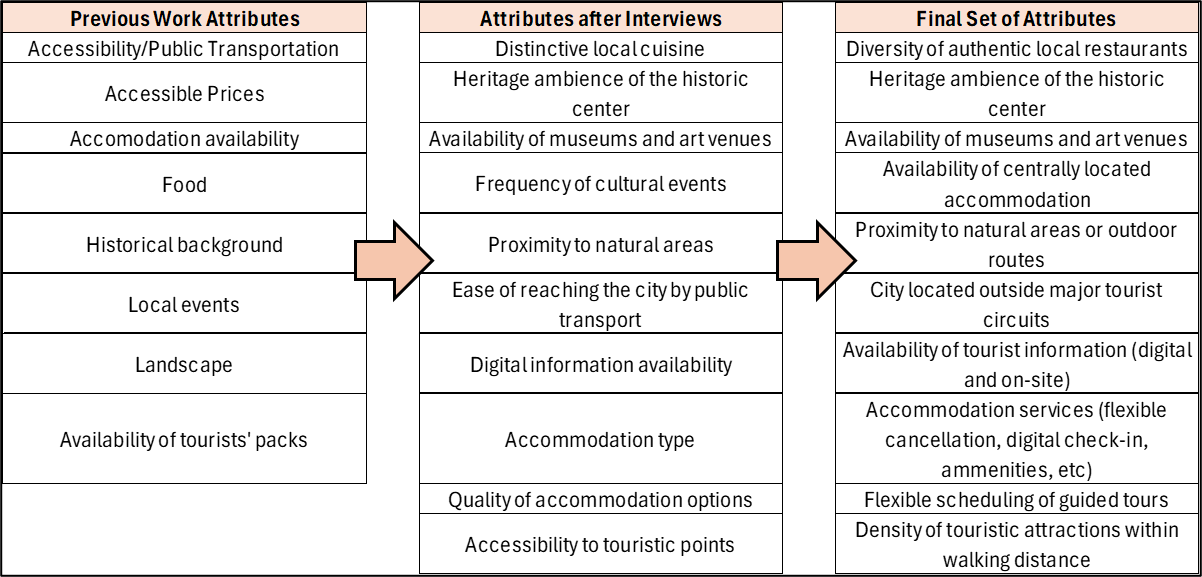
\includegraphics[width=1\textwidth]{Images/Final Set of Attributes.png}
    \captionsetup{font=footnotesize}
    \caption{\textit{Final Set of Attributes. Source: Author’s own elaboration.}}
    \label{fig:final_set_att}
\end{figure}


\section{Quantitative Survey}

\subsection{Methodology}

\subsubsection{Quantitative Survey}

\indent After completing the process of defining the final set of attributes, the quantitative survey (see Appendix~\ref{sec:quantitativesurvey}) was conducted to test this set and identify potential tourist clusters. In addition to asking respondents to rank the attributes according to their preferences, it was important to include Likert-scale questions to serve as a control for attribute preferences, as well as additional questions related to the attributes to further explain touristic behaviour. Some descriptive questions were also incorporated to characterise each cluster more precisely. The survey also included, as an illustrative example, a dedicated section with questions specifically referring to the city under analysis. This section was designed as a template that could be adapted to any destination applying the same methodology. In this study, it was implemented using the reference case of Ascoli Piceno.

\indent The survey was completed by a total of 125 respondents, with the aim of capturing a diverse sample across different age groups, primarily individuals with the ability to plan and undertake trips, such as professionals or even students living in Europe (travel distances are generally shorter compared to larger or more distant regions).

\subsubsection{Ranking vs Likert Scale}

\indent Firstly, after getting the dataset with all the answers, the ranking responses were reorganised so that each attribute corresponded to a separate column, containing the numerical rank assigned by each respondent. To enable comparison with the Likert-scale questions, the ranking values were then inverted (the attribute ranked first was assigned a value of 10, the second a value of 9, and so on) and subsequently rescaled to a 1–5 range. This transformation ensured comparability with the Likert scale, where values range from 1 (strongly disagree) to 5 (strongly agree). 

\indent Once both datasets were aligned on the same scale, a correlation analysis was conducted to evaluate the relationship between the ranking-based preferences and the Likert-scale responses for each attribute. The non-parametric Spearman’s rank correlation coefficient (\(\rho\)) was employed, as it measures the strength and direction of the monotonic relationship between two ranked variables \cite{spearman}. Statistical significance was assessed through p-values, and significance levels were labelled using standard notation (\(*p < 0.05\), \(**p < 0.01\), \(***p < 0.001\), \(****p < 0.0001\)). The pseudocode of the implemented procedure is presented below:

\begin{algorithm}[H]
\caption{Spearman Correlation Analysis}\label{alg:spearmancorr}
\begin{algorithmic}[1]
\Require DataFrames $df\_ranking\_scaled$ and $df\_likert$
\State Initialize empty list $corrs$
\For{each column $i$ in $df\_ranking\_scaled$}
    \State $x \gets df\_ranking\_scaled[:, i]$
    \State $y \gets df\_likert[:, i]$
    \State Compute Spearman correlation: $(\rho, p) \gets spearmanr(x, y)$
    \State Append \texttt{[Attribute, $\rho$, p]} to $corrs$
\EndFor
\State Create DataFrame $result$ from $corrs$
\For{each $p$ in $result[p\_value]$}
    \If{$p < 0.0001$}
        \State Assign significance label: \texttt{`****'}
    \ElsIf{$p < 0.001$}
        \State Assign significance label: \texttt{`***'}
    \ElsIf{$p < 0.01$}
        \State Assign significance label: \texttt{`**'}
    \ElsIf{$p < 0.05$}
        \State Assign significance label: \texttt{`*'}
    \Else
        \State Assign significance label: \texttt{`'}
    \EndIf
\EndFor
\State Round $\rho$ to three decimals and $p$ to four decimals
\Ensure DataFrame $result$ containing attributes, Spearman $\rho$, p-values, and significance labels
\end{algorithmic}
\end{algorithm}

\subsubsection{Defining Optimal K}

\indent The ten final attributes, using their original ranking values, were employed as input variables for the clustering analysis. The inverted and rescaled versions were used exclusively for validation purposes, such as the consistency check with the Likert-scale questions.

\indent In the previous work, the clustering procedure was conducted using the K-Means algorithm; however, given the ordinal nature of the ranking data, a more suitable combination involves the Gower distance and the K-Medoids algorithm. Unlike K-Means, which relies on Euclidean distance and is therefore appropriate only for continuous and numerical data, K-Medoids is more robust to noise and can handle mixed or ordinal data types, as it minimizes a sum of pairwise dissimilarities rather than squared distances \cite{KaufmanRousseeuw1990}. The use of Gower distance enables the measurement of similarity across variables of different scales and types, including ordinal and categorical attributes \cite{Gower1971}. This makes the Gower + K-Medoids approach particularly suitable for clustering survey data, as it preserves the relative ordering of attributes while maintaining interpretability and robustness to outliers \cite{Hennig2015, Podani1999}.

\indent To determine the optimal number of clusters ($k$), three complementary methods were applied:

\begin{itemize}
    \item Elbow method (Algorithm~\ref{alg:bertopic} in Appendix~\ref{sec:textmining}): evaluates the reduction in within-cluster dissimilarity as $k$ increases \cite{elbow}.
    \item Silhouette score (Algorithm~\ref{alg:bertopic} in Appendix~\ref{sec:textmining}): assesses how well each observation fits within its assigned cluster compared to others \cite{Rousseeuw1987}.
    \item Davies–Bouldin Index (DBI) (Algorithm~\ref{alg:bertopic} in Appendix~\ref{sec:textmining}): measures intra-cluster cohesion and inter-cluster separation \cite{DaviesBouldin1979}.
\end{itemize}

The combination of these criteria ensured a robust and data-driven determination of the most appropriate clustering structure.

\subsubsection{Principal Component Analysis (PCA)}

\indent After completing the clustering analysis, the cluster labels were adjusted for clarity by reindexing them from 0–3 to 1–4. This change was made solely for presentation purposes, as it provides a more intuitive numbering convention when discussing and visualising the resulting groups.

\indent To further explore the internal structure of the data and assess the separability of the identified clusters, a Principal Component Analysis (PCA) was conducted. PCA is a widely used linear dimensionality reduction technique that transforms the original variables into a new set of uncorrelated components, ordered according to the amount of variance they explain in the dataset \cite{Jolliffe2002}. This transformation allows high-dimensional data to be represented in two or three dimensions while retaining as much of the underlying information as possible.

\indent In this study, PCA was applied to the scaled ranking data to evaluate whether the resulting components could visually distinguish the clusters obtained through the Gower + K-Medoids procedure. The main objective was not dimensionality reduction for analysis itself, but rather to obtain a visual representation that could help interpret and validate the clustering results.



\subsection{Results}

\subsubsection{Quantitative Survey}

\indent The final quantitative survey collected a total of 125 responses. This sample provides a diverse representation of individuals from different age groups, genders, occupations, and geographical regions, allowing for a broad perspective on tourism preferences and behaviour patterns.

\indent In terms of age distribution (see Figure~\ref{fig:answers_by_age}), the majority of respondents were between 26 and 35 years old (51 participants), followed by those aged 18–25 (26 participants) and over 55 (19 participants). This distribution indicates a predominance of young adults.

\begin{figure}[ht]
    \centering
    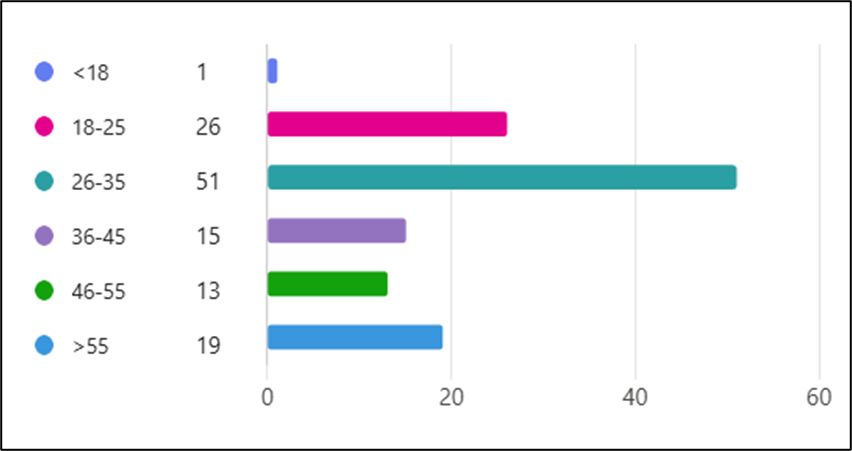
\includegraphics[width=0.7\textwidth]{Images/Quantitative Survey/answers by age.png}
    \captionsetup{font=footnotesize}
    \caption{\textit{Number of respondents by agre range. Source: Author’s own elaboration.}}
    \label{fig:answers_by_age}
\end{figure}

\indent Regarding gender (Figure~\ref{fig:answers_by_gender}), the sample shows a relatively balanced representation across genders.

\begin{figure}[ht]
    \centering
    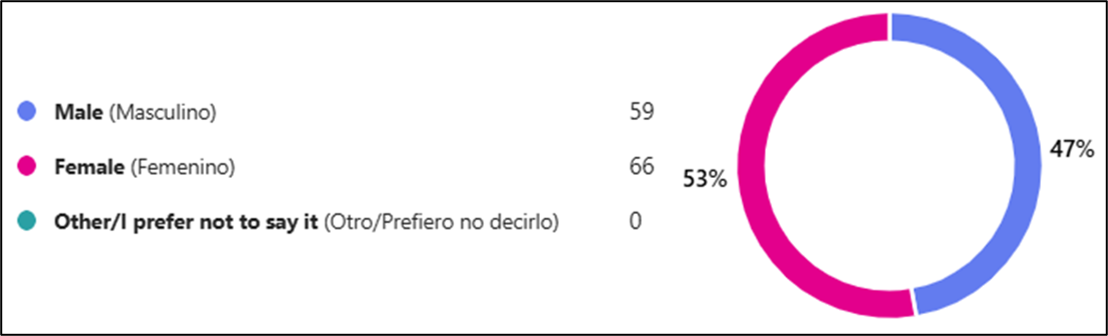
\includegraphics[width=0.7\textwidth]{Images/Quantitative Survey/answers by gender.png}
    \captionsetup{font=footnotesize}
    \caption{\textit{Number of respondents by gender. Source: Author’s own elaboration.}}
    \label{fig:answers_by_gender}
\end{figure}

\indent With respect to the region of residence the survey was mainly aimed to get respondents from South America and Europe. This last case was opened between Italian and Non-Italian respondents, as mentioned before, the case of reference is Ascoli Piceno, and this is an important difference as it can compare national vs international tourism. As shown in Figure~\ref{fig:answers_by_residence}, most respondents were located in South America (54) and Italy (44), followed by participants from Europe excluding Italy (23). This distribution aligns with the recruitment strategy, which focused on reaching individuals familiar with the European travel context while maintaining an international perspective.

\begin{figure}[ht]
    \centering
    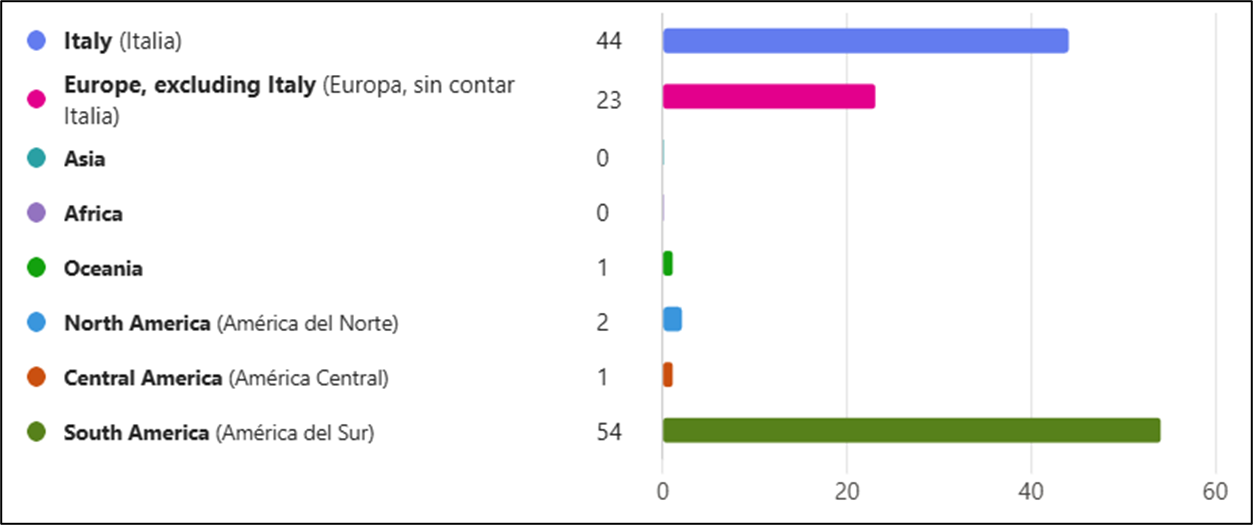
\includegraphics[width=0.7\textwidth]{Images/Quantitative Survey/answers by residence.png}
    \captionsetup{font=footnotesize}
    \caption{\textit{Number of respondents by residence. Source: Author’s own elaboration.}}
    \label{fig:answers_by_residence}
\end{figure}

\indent Finally, regarding occupational status (Figure~\ref{fig:answers_by_profession}), employed individuals accounted for the largest share of the sample (56 participants), followed by students (31) and self-employed professionals (27). This variety of employment situations reflects different travel capacities and motivations among respondents.

\begin{figure}[ht]
    \centering
    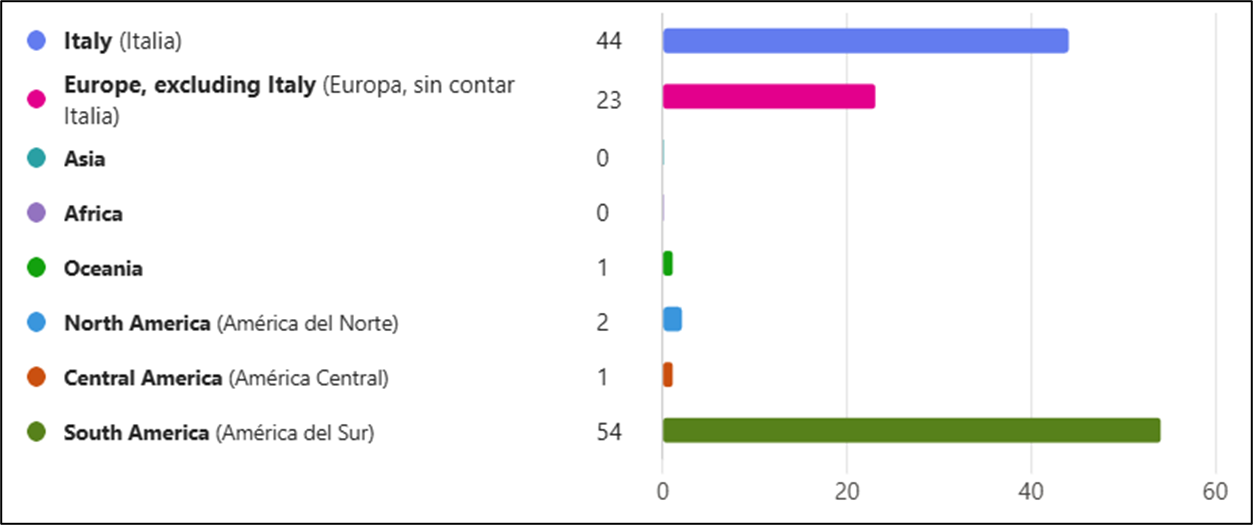
\includegraphics[width=0.7\textwidth]{Images/Quantitative Survey/answers by residence.png}
    \captionsetup{font=footnotesize}
    \caption{\textit{Number of respondents by profession. Source: Author’s own elaboration.}}
    \label{fig:answers_by_profession}
\end{figure}

\indent Overall, the demographic composition of the sample ensures a balanced mix of respondents across key sociodemographic variables, providing a solid basis for the subsequent analysis of tourist segmentation and behavioural patterns.

\subsubsection{Ranking vs Likert Scale}

\indent The inclusion of Likert-scale questions proved valuable as a control mechanism to assess whether respondents answered the ranking section consciously rather than arbitrarily. As shown in Figure~\ref{fig:spearman_results}, the correlation between the ranking values and their corresponding Likert-scale evaluations was both positive and statistically significant for all attributes, with Spearman’s $\rho$ values ranging between 0.40 and 0.60. This indicates a consistent alignment between the two measures, confirming that participants generally evaluated the attributes coherently. The only exception was the manually modified attribute, ``City located outside major tourist circuits'', which displayed a weaker correlation ($\rho = 0.208$, $p = 0.020$), likely reflecting its distinct conceptual framing compared to the rest of the attributes that were correclty obtained from the methodology suggested in this research.

\begin{figure}[ht]
    \centering
    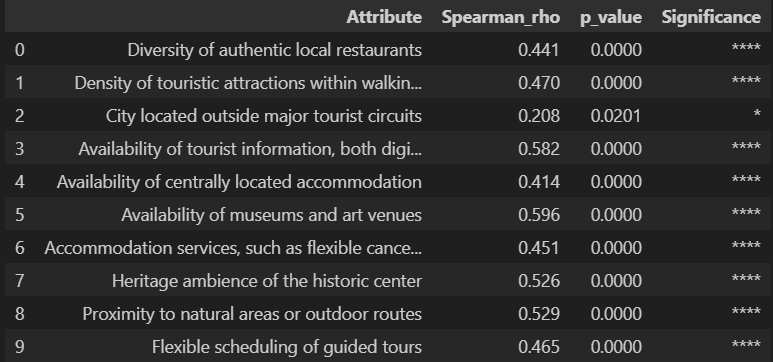
\includegraphics[width=0.7\textwidth]{Images/Quantitative Survey/rank_likert_corr.png}
    \captionsetup{font=footnotesize}
    \caption{\textit{Spearman correlation between ranking and Likert-scale responses. Source: Author’s own elaboration.}}
    \label{fig:spearman_results}
\end{figure}

\indent Although these results validate the reliability of the ranking data, the moderate level of correlation suggests that the Likert scale is less informative for segmentation purposes. As illustrated in Figure~\ref{fig:likert_distribution}, most respondents tended to rate nearly all attributes as important or very important (values 3–5 on the scale). This pattern of limited variability indicates that the Likert responses alone would not provide sufficient discrimination power for clustering, as the majority of participants expressed uniformly positive evaluations across attributes.

\begin{figure}[ht]
    \centering
    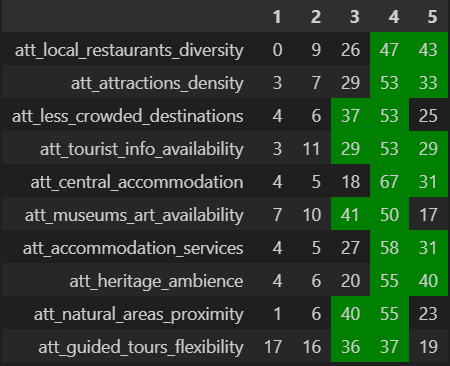
\includegraphics[width=0.5\textwidth]{Images/Quantitative Survey/likert_count.png}
    \captionsetup{font=footnotesize}
    \caption{\textit{Likert-scale count. Source: Author’s own elaboration.}}
    \label{fig:likert_distribution}
\end{figure}

\subsubsection{Defining Optimal K}

\indent Based on the results obtained from the clustering validation methods, the optimal number of clusters was determined to be $k = 4$. As shown in Figure~\ref{fig:elbow_plot}, the Elbow method did not display a sharply defined inflection point; however, a noticeable change in the slope was observed starting at $k = 4$, with a similar variation at $k = 5$. This suggested that four and 5 clusters might represent a reasonable balance between model simplicity and internal cohesion. Using more than one validation method allows a better definition of $k$.

\begin{figure}[ht]
    \centering
    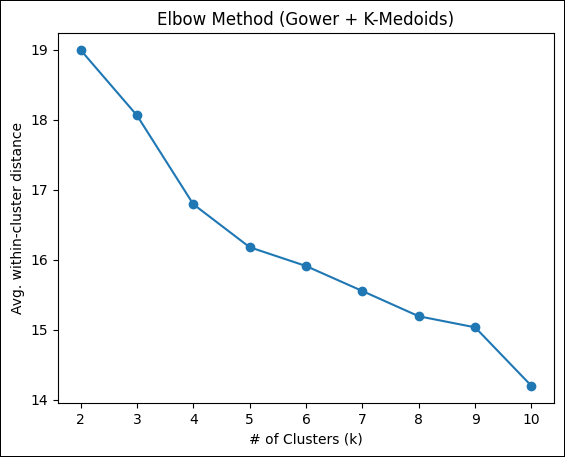
\includegraphics[width=0.7\textwidth]{Images/Quantitative Survey/elbow_method.png}
    \captionsetup{font=footnotesize}
    \caption{\textit{Elbow plot. Source: Author’s own elaboration.}}
    \label{fig:elbow_plot}
\end{figure}

\indent The Silhouette score analysis (Figure~\ref{fig:silhouette_plot}) provided clearer evidence, indicating $k = 4$ as the most appropriate choice, with the highest score of $0.087$. This result shows that, although the clusters are not perfectly separated—an expected outcome in behavioural data—the overall structure still reflects a meaningful segmentation of tourist preferences.

\begin{figure}[ht]
    \centering
    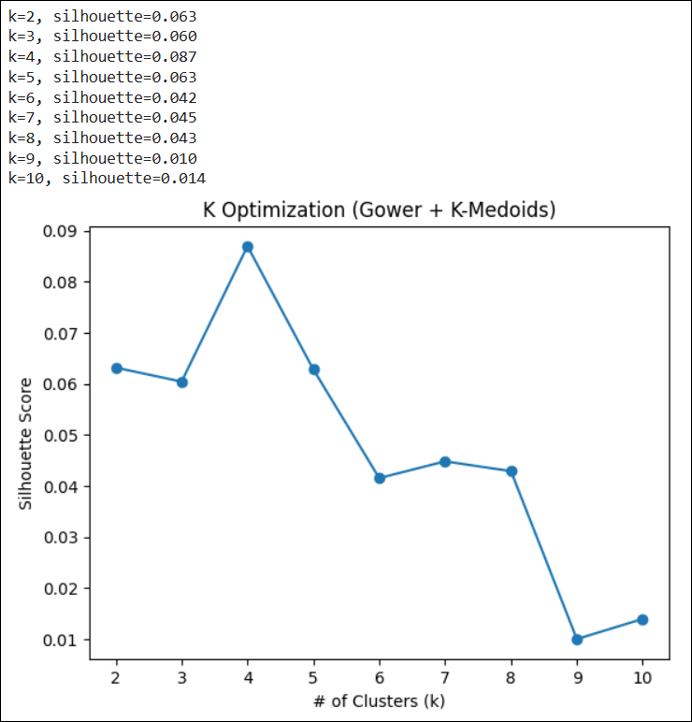
\includegraphics[width=0.7\textwidth]{Images/Quantitative Survey/silhouette.png}
    \captionsetup{font=footnotesize}
    \caption{\textit{Silhouette scores and plot. Source: Author’s own elaboration.}}
    \label{fig:silhouette_plot}
\end{figure}

\indent The Davies–Bouldin Index (DBI) supported this conclusion, with the lowest index value also occurring at $k = 4$ (DBI = 3.088), compared with higher values for other configurations as shown in igure~\ref{fig:dbi_scores}. Taken together, the three methods consistently indicated that the most coherent and stable partition of the data corresponds to four clusters, which was therefore adopted for the subsequent analyses.

\begin{figure}[ht]
    \centering
    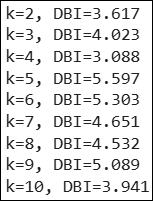
\includegraphics[width=0.2\textwidth]{Images/Quantitative Survey/dbi.png}
    \captionsetup{font=footnotesize}
    \caption{\textit{DBI scores. Source: Author’s own elaboration.}}
    \label{fig:dbi_scores}
\end{figure}

\indent Overall, after applying multiple validation methods to determine the optimal number of clusters, the analysis concluded that the most appropriate solution was $k = 4$. The final segmentation included clusters as follows:

\begin{itemize}
    \item Cluster~1: 35 (28\%).
    \item Cluster~2: 36 (28\%).
    \item Cluster~3: 23 (18\%).
    \item Cluster~4: 31 (24\%).
\end{itemize}


\indent Figure~\ref{fig:clusters_means} presents the mean values of the segmentation variables by cluster, illustrating how the importance assigned to each attribute varies among groups. As shown, Cluster~1 exhibits relatively low mean values across most attributes, suggesting a segment that places less emphasis on cultural and informational aspects of the destination. Cluster~2, on the other hand, scores higher on attributes related to culture and heritage, particularly the availability of museums and the historic ambience, indicating a preference for culturally rich destinations. Cluster~3 stands out for prioritising convenience and flexibility, showing higher scores for accommodation services and the diversity of local restaurants, and moderately high values for proximity to outdoor areas. Finally, Cluster~4 is characterised by high scores across almost all variables, especially for attributes such as the density of tourist attractions, flexible guided tours, and accommodation amenities, suggesting a highly engaged segment that values accessibility, variety, and comfort during travel.

\begin{figure}[ht]
    \centering
    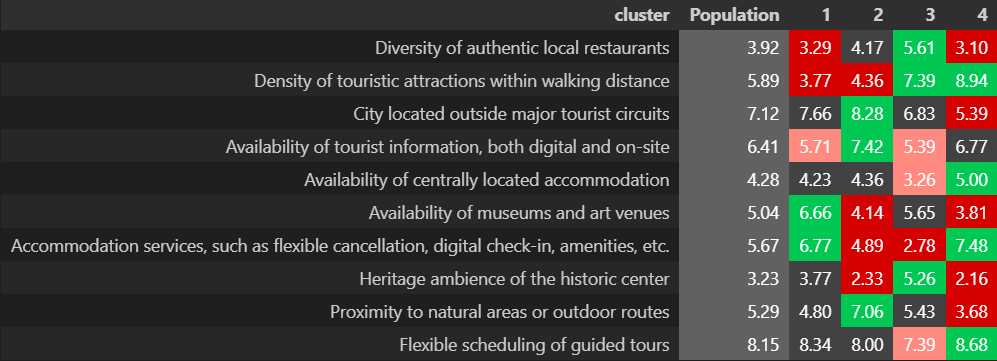
\includegraphics[width=0.9\textwidth]{Images/Quantitative Survey/variables by segmentation.png}
    \captionsetup{font=footnotesize}
    \caption{\textit{Means of segmentation variables by segment. Source: Author’s own elaboration.}}
    \label{fig:clusters_means}
\end{figure}

\subsubsection{Dimensionality Reduction: Principal Component Analysis (PCA)}

\indent Although PCA was initially performed to explore potential data reduction and visualization, its explanatory power proved insufficient for clear interpretation. The first six principal components, as shown in Figure~\ref{fig:accumm_pca}, together explained most of the variance in the dataset, but no two-dimensional or three-dimensional representation could adequately capture the underlying structure. For this reason, PCA was not useful for graphical visualization of clusters (see Figure~\ref{fig:pca_clusters} in Appendix~\ref{sec:pca_clustering}), and the interpretation relied instead on clustering metrics and attribute-level analysis.

\begin{figure}[ht]
    \centering
    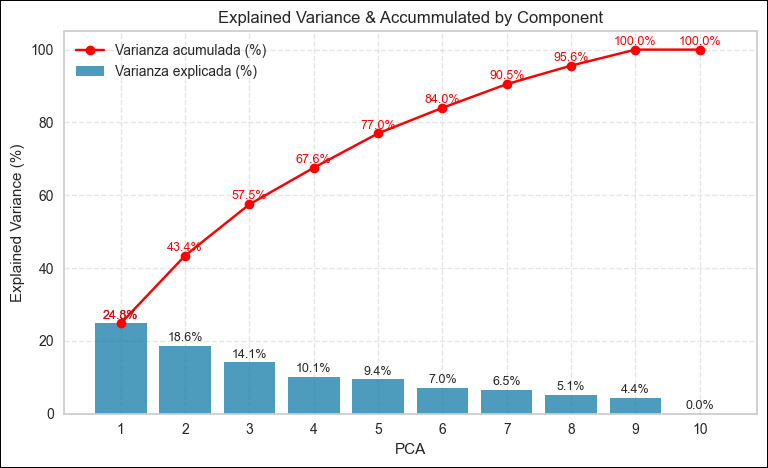
\includegraphics[width=0.9\textwidth]{Images/Quantitative Survey/pca.png}
    \captionsetup{font=footnotesize}
    \caption{\textit{Cumulative Explained Variance (PCA). Source: Author’s own elaboration.}}
    \label{fig:accumm_pca}
\end{figure}


\chapter{Discussion}

\section{Qualitative Approach}

\indent In the Chapter 2, section 2.1, it was described some potential risks that may appear when developing and conducting a qualitative interview. One of them is compliance bias, where responses could be influenced by participants’ personal impression of what they were expected to answer. This was addressed by avoiding any disclosure of the project’s purpose and by formulating questions without references to what other people might do. Interviewees were simply invited to participate in an interview, and once the session began, they were explained only that the topic was tourism before moving directly to the questions. The approach followed the principles of the ``Mom Test" described by Rob Fitzpatrick, where participants are asked ``questions that even your mom could answer honestly" \cite{massimo}. Another potential risk concerned offset bias, in which participants might be forced to reflect on problems they were not aware of or to consider certain issues as more complex than they normally would. This was mitigated by avoiding the introduction of unfamiliar terms and by ensuring that the evaluation of a problem remained entirely with the interviewee. Finally, speculation bias was the last potential risk mentioned, where participants could be asked to predict their own behaviour in hypothetical future situations. Since people are not generally good at determining what they would do in an hypothetical scenario that never happened to them, participants were instead asked about past and present experiences, and to tell ``stories” about what they normally do and don’t do. In this way, deeper questions were asked progressively and with patience, as individuals are not able to correctly determine the underlying reasons for their own behavior \cite{massimo}. It is important to note that this exercise did not involve speculation bias, since participants were not asked to predict hypothetical future behaviours. Instead, they were asked to apply their usual, real-life trip planning process to the case of Ascoli Piceno, following the same steps, tools, and resources they normally use.

\indent In this way, the approach sought to address the limitations of reliability and subjectivity. On the other hand, although the process was labour-intensive, only ten interviews were conducted, and generalisability was not considered a limitation, since the main purpose of this first stage was to generate a list of attributes to be tested in the following stages, and with the final survey, the larger sample makes generalisation possible.

\chapter{Conclusion}

\newpage

\sloppy
\begin{thebibliography}{9}
\raggedright

\bibitem{unwtocovid}
"Tourism and COVID-19 – Unprecedented Economic Impacts", \textit{World Tourism Organization (UN Tourism)}, n.d. \url{https://www.unwto.org/tourism-and-covid-19-unprecedented-economic-impacts}.

\bibitem{unwtoppt}
"World Tourism Barometer (PPT version)", \textit{World Tourism Organization (UN Tourism)}, January 2025. \url{https://webunwto.s3.eu-west-1.amazonaws.com/s3fs-public/2024-01/barometer-turism-data-ppt-jan24.pdf?VersionId=ua6xuwZCeveZWEzbIFVP5eXUmGszXhXs}

\bibitem{unwtodash}
"UN Tourism Data Dashboard", \textit{World Tourism Organization (UN Tourism)}, n.d. \url{https://www.unwto.org/tourism-data/un-tourism-tourism-dashboard}.

\bibitem{italia_it}
"Ascoli Piceno, the city of a hundred towers and good living", \textit{Italia.it – Official Italian Tourism Website}, n.d. \url{https://www.italia.it/en/marche/ascoli-piceno/guide-history-facts}

\bibitem{istat}
"Movimento dei clienti (arrivi e presenze) negli esercizi ricettivi per tipologia ricettiva, residenza dei clienti e comune di destinazione", \textit{ISTAT – Italian National Institute of Statistics}, n.d. \url{https://esploradati.istat.it/databrowser/#/it/dw/categories/IT1,Z0700SER,1.0/SER_TOURISM/SER_TOURISM_RELATED_FILES}.

\bibitem{vw_model}
Rebecca Shaddix. "How To Price Your Product: A Guide To The Van Westendorp Pricing Model", \textit{Forbes}, January 9, 2023. \url{https://www.forbes.com/sites/rebeccasadwick/2020/06/22/how-to-price-products/}

\bibitem{tashakkori}
A. Tashakkori, and C. Teddlie. "Mixed methodology: Combining qualitative and quantitative approaches", \textit{Sage Publications, Inc.}, 1998.

\bibitem{creswell}
J. W. Creswell. "Research design: Qualitative \& quantitative approaches", \textit{Sage Publications, Inc.}, 1994.

\bibitem{creswelletal}
J.W. Creswell, A.C. Klassen, V.L. Plano Clark, and K. Clegg Smith. "Best Practices for Mixed Methods Research in the Health Sciences", \textit{Office of Behavioral and Social Sciences Research (OBSSR)}, n.d. \url{https://obssr.od.nih.gov/sites/obssr/files/Best_Practices_for_Mixed_Methods_Research.pdf}

\bibitem{finnetal}
M. Finn, M. Elliott-White, and M. Walton. "Tourism and Leisure Research Methods: Data Collection, Analysis and Interpretation", \textit{Pearson Education Ltd.}, 2000.

\bibitem{mcdowell}
I. McDowell, and L. MacLean. "Blending qualitative and quantitative study methods in health services research", 1998.

\bibitem{scribbr}
Pritha Bhandari. "What Is Qualitative Research? | Methods \& Examples", \textit{Scribbr}, January 14, 2025. \url{https://www.scribbr.com/methodology/qualitative-research/?utm_source=chatgpt.com}

\bibitem{amaratunga}
D. Amaratunga, D. Baldry, M. Sarshar, and R. Newton. "Qualitative and quantitative research in the built environment: application of "mixed" research approach", 2002.

\bibitem{gilmore}
Audrey Gilmore, and David Carson. "Integrative qualitative methods in a services context", \textit{University of Ulster}, November, 1996.

\bibitem{allan}
G. Allan, and C. Skinner. "Qualitative Handbook for Research Students in the Social Sciences", \textit{Palmer Press}, 1991.

\bibitem{lincoln}
Yvonna S. Lincoln, and Egon G. Guba. "Naturalistic Inquiry", \textit{Sage}, 1985.

\bibitem{deruyter}
K. de Ruyter, and N. Scholl. "Qualitative Market Research: An International Journal", 1998.

\bibitem{veal}
A. J. Veal. "Research Methods for Leisure and Tourism: A Practical Guide", \textit{Financial Times Management}, 1997.

\bibitem{murphyblack}
Tricia Murphy-Black. "The research process: a mind map", \textit{British Journal of Midwifery}, November, 1994.

\bibitem{scribbrquant}
Pritha Bhandari. "What Is Quantitative Research? | Definition, Uses \& Methods", \textit{Scribbr}, June 22, 2023. \url{https://www.scribbr.com/methodology/quantitative-research/}

\bibitem{bernard}
H. Bernard. "Social Research Methods: Qualitative and Quantitative Approaches", \textit{Sage, Thousand Oaks}, 2000.

\bibitem{neuman}
William Lawrence Neuman. "Social Research Methods: Qualitative and Quantitative Approaches", \textit{Sage Publications}, 1991.

\bibitem{cooper}
Donald R. Cooper, amd Pamela S. Schindler. "Business Research Methods", \textit{McGraw-Hill}, 1998.

\bibitem{carsonetal}
D. Carson, Audrey Gilmore, Chad Perry, and Kjell Grønhaug. "Qualitative Market Research", \textit{Sage Publications Ltd}, January, 2001.

\bibitem{jick}
Todd D. Jick. "Mixing Qualitative and Quantitative Methods: Triangulation in Action", \textit{Sage Publications, Inc.}, December, 1979.

\bibitem{whisperx}
Max Bain. "WhisperX", \textit{GitHub repository}, June 27, 2025. \url{https://github.com/m-bain/whisperX?utm_source=chatgpt.com}

\bibitem{massimo}
Massimo Aliberti. "Customer - Problem Interview", \textit{Imperial College London}, 2017. \url{https://drive.google.com/file/d/1pa8EQhqbvVkq0DwAQcdvMnTzyhnwMM4x/view?pli=1}

\bibitem{destinationimg}
Seyhmus Baloglu and Ken W. McCleary. "A Model of Destination Image Formation", \textit{Annals of Tourism Research}, 1999.

\bibitem{clustering}
Juho Pesonen and Antti Honkanen. "Using cluster analysis to segment tourists: response-style effects", \textit{Matkailututkimus}, 2014.

\bibitem{discretechoice}
Astrid Kemperman. "A review of research into discrete choice experiments in tourism: Launching the Annals of Tourism Research Curated Collection on Discrete Choice Experiments in Tourism", \textit{Annals of Tourism Research}, 2021.

\bibitem{conjointaltin}
Altin, M. "Conjoint Analysis in Tourism", \textit{Springer Nature}, 2023.

\bibitem{hypotheticalbias}
David A. Hensher. "Hypothetical bias, choice experiments and willingness to pay", \textit{Elsevier}, 2010.

\bibitem{touristheterogenity}
Lingling Wu, Junyi Zhang, and Akimasa Fujiwara . "Representing tourists’ heterogeneous choices of destination and travel party with an integrated latent class and nested logit model", \textit{Elsevier}, 2011.

\bibitem{textmining}
Qing Zhu, Yiqiong Wu, Yuze Li, and Renxian Zuo, ``A Text Mining Based Approach for Mining Customer Attribute Data on Undefined Quality Problem'' \textit{The Seventeenth Wuhan International Conference on E-Business}, 2018.

\bibitem{ghani}
Rayid Ghani, Katharina Probst, Yan Liu, Marko Krema, and Andrew Fano, ``Text Mining for Product Attribute Extraction'' \textit{SIGKDD Explorations. Volume 8, Issue 1}, 2006.

\bibitem{datamining}
Er. Rupampreet Kaur and Er.Kiranbir Kaur, ``Data Mining on Customer Segmentation: A Review'' \textit{International Journal of Advanced Research in Computer Science. Volume 8}, May-June 2017.

\bibitem{unlockinginsights}
Na Li, Yu-Tao Liu, and Zhan Chen, ``Unlocking insights: integrated text mining and interpretive structural modeling for enhanced user review analysis'' \textit{PeerJ Computer Science}, 2024.

\bibitem{bookingdata}
The Devastator. \textit{Booking.com Hotel Reviews}. Kaggle, 2019. Available at: \url{https://www.kaggle.com/datasets/thedevastator/booking-com-hotel-reviews?resource=download}.

\bibitem{airbnbdata}
"Get the Data". \textit{Inside Airbnb}. Available at: \url{https://insideairbnb.com/get-the-data/}.

\bibitem{cld2}
CLD2Owners. "Compact Language Detector 2". \textit{Github}, 2015. Available at: \url{https://github.com/CLD2Owners/cld2}.

\bibitem{vanwestern}
Rebecca Shaddix. "How To Price Your Product: A Guide To The Van Westendorp Pricing Model". \textit{Forbes}, June 22, 2020. \url{https://www.forbes.com/sites/rebeccasadwick/2020/06/22/how-to-price-products/}.

\bibitem{spearman}
"Spearman's Rank-Order Correlation". \textit{Laerd Statistics}, n.d. \url{https://statistics.laerd.com/statistical-guides/spearmans-rank-order-correlation-statistical-guide.php}.

\bibitem{KaufmanRousseeuw1990}
Leonard Kaufman, and Peter Rousseeuw, ``Finding Groups in Data: An Introduction To Cluster Analysis'' \textit{Wiley}, January 1990.

\bibitem{Gower1971}
J. C. Gower, ``A General Coefficient of Similarity and Some of Its Properties'' \textit{International Biometric Society. Vol. 27, No. 4 (Dec., 1971), pp. 857-871}, December 1971.

\bibitem{Hennig2015}
Christian Hennig, ``What are the true clusters?'' \textit{Pattern Recognition Letters 27}, February 2015.

\bibitem{Podani1999}
Janos Podani, ``Extending Gower's General Coefficient of Similarity to Ordinal Characters'' \textit{Taxon 48(2):331}, May 1999.

\bibitem{elbow}
ZalaRushirajsinh, "The Elbow Method: Finding the Optimal Number of Clusters". \textit{Medium}, November 4, 2023. \url{https://medium.com/@zalarushirajsinh07/the-elbow-method-finding-the-optimal-number-of-clusters-d297f5aeb189}.

\bibitem{Rousseeuw1987}
Peter Rousseeuw, ``Silhouettes: A graphical aid to the interpretation and validation of cluster analysis'' \textit{Journal of Computational and Applied Mathematics 20:53-65}, November 1987.

\bibitem{DaviesBouldin1979}
Don Bouldin, ``A Cluster Separation Measure'' \textit{IEEE Transactions on Pattern Analysis and Machine Intelligence PAMI-1(2):224 - 227}, May 1979.

\bibitem{Jolliffe2002}
I. T. Jolliffe, ``Principal Componentes Analysis, Second Edition'' \textit{Springer Series in Statistics}, 2002.


\end{thebibliography}

\newcounter{appendixsection}
\renewcommand{\theappendixsection}{\Alph{appendixsection}}

\newcommand{\appendixsection}[2][]{%
  \refstepcounter{appendixsection}%
  \section*{\theappendixsection. #2}%
  \addcontentsline{toc}{section}{\theappendixsection. #2}%
  \ifx&#1&%
  \else%
    \label{#1}%
  \fi%
}

\chapter*{Appendix}
\addcontentsline{toc}{chapter}{Appendix}


\appendixsection[sec:previouswork]{Example of Qualitative Interview from Previous Project}
\input{Material/2. Interviews & SUrveys/1. Qualitative Interview/Example Qualitative Interview - Previous Porject.txt}


\appendixsection[sec:interview]{Example of Qualitative Interview from Actual Thesis}
\input{Material/2. Interviews & Surveys/1. Qualitative Interview/1. Interview 31-07-2025 18-15/1. Interview 31-07-2025 18-15 (ENGLISH).txt}


\includepdf[
  pages=1,
  pagecommand={\appendixsection[sec:interviewnotes]{Qualitative Interview Notes}}
]{Material/2. Interviews & Surveys/1. Qualitative Interview/Attributes (for thesis).pdf}

\includepdf[
  pages=2-,
  pagecommand={}
]{Material/2. Interviews & Surveys/1. Qualitative Interview/Attributes (for thesis).pdf}

{
\setlength{\textfloatsep}{5pt}
\setlength{\intextsep}{5pt}
\setlength{\floatsep}{5pt}
\setlength{\parskip}{0pt}

\titlespacing*{\section}{0pt}{*1}{15pt}
\appendixsection[sec:textmining]{Pseudocodes for Text Mining}

\begin{algorithm}[H]
\caption{text\_pipeline}\label{alg:textpipeline}
\begin{algorithmic}[1]
\Require DataFrame $df$, input column name $input\_col$, and stopword removal flag
\For{each text in $df[input\_col]$}
    \If{text is missing}
        \State Append an empty token list and continue
    \EndIf
    \State Convert text to lowercase
    \State Remove all non-alphanumeric characters (keep spaces)
    \State Tokenize and lemmatize the text
    \If{stopword removal is enabled}
        \State Keep only alphabetic tokens that are not stopwords
    \Else
        \State Keep all alphabetic tokens
    \EndIf
    \State Append the resulting tokens to the list of processed texts
\EndFor
\State Add a new column \texttt{final\_tokens} to the DataFrame containing the processed tokens
\Ensure DataFrame $df$ with a column of cleaned, lemmatized tokens
\end{algorithmic}
\end{algorithm}

\vspace{-0.1em}

\begin{algorithm}[H]
\caption{chunk\_text}\label{alg:chunktext}
\begin{algorithmic}[1]
\Require Text string $text$, number of sentences per chunk $n\_sentences = 6$
\State Tokenise $text$ into sentences using \texttt{sent\_tokenize} from NLTK
\State Initialize empty list $chunks$
\For{$i \gets 0$ to length($sentences$) step $n\_sentences$}
    \State $chunk \gets$ concatenate sentences[$i : i+n\_sentences$]
    \If{length($chunk$) $>$ 30}
        \State Append $chunk$ to $chunks$
    \EndIf
\EndFor
\Ensure List $chunks$ containing all valid text segments
\end{algorithmic}
\end{algorithm}

\vspace{-0.1em}

\begin{algorithm}[H]
\caption{compute\_tfidf\_ngrams}\label{alg:compute_tfidf_ngrams}
\begin{algorithmic}[1]
\Require Data frame $df\_cleaned\_interviews$ with column \texttt{final\_tokens}, custom stopword list $custom\_stops$
\State Initialize empty list $docs$
\For{each row in $df\_cleaned\_interviews$}
    \State Concatenate tokens in \texttt{final\_tokens} into a single string
    \State Append the resulting string to $docs$
\EndFor

\Comment{--- Compute TF-IDF for unigrams ---}
\State Initialize $vectorizer\_words \gets$ TfidfVectorizer(ngram\_range=(1,1), stop\_words=$custom\_stops$)
\State Fit and transform $docs$ with $vectorizer\_words$ to obtain matrix $X\_words$
\State Compute mean TF-IDF per term: $tfidf\_means \gets mean(X\_words, axis=0)$
\State Extract feature names: $words \gets vectorizer\_words.get\_feature\_names\_out()$
\State Sort indices by decreasing importance: $top\_words\_idx \gets argsort(tfidf\_means)[::-1]$
\State Create table $top\_words$ with columns ``ngram'' and ``tfidf'' using top 30 entries

\Comment{--- Compute TF-IDF for bigrams ---}
\State Initialize $vectorizer\_bigrams \gets$ TfidfVectorizer(ngram\_range=(2,2), stop\_words=$custom\_stops$)
\State Fit and transform $docs$ with $vectorizer\_bigrams$ to obtain $X\_bigrams$
\State Compute mean TF-IDF per bigram: $tfidf\_means\_bigrams \gets mean(X\_bigrams, axis=0)$
\State Extract feature names: $bigrams \gets vectorizer\_bigrams.get\_feature\_names\_out()$
\State Sort indices: $top\_bigrams\_idx \gets argsort(tfidf\_means\_bigrams)[::-1]$
\State Create table $top\_bigrams$ with columns ``bigram'' and ``tfidf'' using top 20 entries

\Comment{--- Compute TF-IDF for trigrams ---}
\State Initialize $vectorizer\_trigrams \gets$ TfidfVectorizer(ngram\_range=(3,3), stop\_words=$custom\_stops$)
\State Fit and transform $docs$ with $vectorizer\_trigrams$ to obtain $X\_trigrams$
\State Compute mean TF-IDF per trigram: $tfidf\_means\_trigrams \gets mean(X\_trigrams, axis=0)$
\State Extract feature names: $trigrams \gets vectorizer\_trigrams.get\_feature\_names\_out()$
\State Sort indices: $top\_trigrams\_idx \gets argsort(tfidf\_means\_trigrams)[::-1]$
\State Create table $top\_trigrams$ with columns ``trigram'' and ``tfidf'' using top 20 entries

\Ensure Data frames $top\_words$, $top\_bigrams$ and $top\_trigrams$ contain the most relevant $n$-grams by average TF-IDF score
\end{algorithmic}
\end{algorithm}

\vspace{-0.1em}

\begin{algorithm}[H]
\caption{bertopic\_implementation}\label{alg:bertopic}
\begin{algorithmic}[1]
\Require Data frame $df\_interviews$ containing column ``text''
\State Initialize empty lists $documents$ and $origin$
\For{each row $(idx, text)$ in $df\_interviews$}
    \State $chunks \gets$ \texttt{chunk\_text}($text$)
    \State Append all $chunks$ to $documents$
    \State Append $idx$ to $origin$ for each $chunk$
\EndFor

\State Load sentence embedding model \texttt{all-MiniLM-L6-v2} from SentenceTransformers
\State Compute embeddings for all $documents$
\State Define custom stopword list combining English stopwords and domain-specific fillers
\State Configure \texttt{TfidfVectorizer} with token pattern $[a-zA-Z]\{4,\}$ and $min\_df = 2$
\State Initialize \texttt{KeyBERTInspired} as the representation model

\State Initialize BERTopic model with:
\begin{itemize}
    \item embedding\_model = MiniLM
    \item representation\_model = KeyBERTInspired
    \item vectorizer\_model = TF-IDF
    \item low\_memory = True
    \item min\_topic\_size = 8
    \item verbose = True
\end{itemize}

\State Fit BERTopic on $documents$ using the generated embeddings
\State Obtain topic assignments $topics$ and their probabilities $probs$
\Ensure Trained BERTopic model and topic distribution across text segments
\end{algorithmic}
\end{algorithm}
}

\appendixsection[sec:chatgpt_prompts]{Prompts for ChatGPT}

\noindent\fbox{
  \parbox{0.95\linewidth}{
  \small
  \textbf{Prompt used:}\\[4pt]
  \textit{I'm going to send you several text files. I want you to read them carefully and then give me a detailed analysis that includes:
  \begin{itemize}\setlength{\itemsep}{2pt}\setlength{\topsep}{2pt}
    \item A list of specific tourism attributes (\emph{in English}) found in each interview (not general ones like price or accommodation).
    \item The frequency of each attribute (across a total of 10 interviews).
    \item A table showing the attributes in English, their frequency, and which interviews they appear in.
  \end{itemize}
  When I send you the files, confirm that you’ve read them, and then start the analysis. Don’t write anything until I confirm that I’ve sent all the files.}}}

\vspace{0.5em}

\noindent\fbox{
  \parbox{0.95\linewidth}{
  \small
  \textbf{Refinement prompt:}\\[4pt]
  \textit{Continuing with this, it’s important to understand that sometimes an attribute can be ambiguous for different respondents. For example, if I include “Historical architecture \& monuments,” it’s not clear whether it refers to the availability of monuments, the presence of a historic center, etc.\\[4pt]
  That’s why I need you to conclude with more detailed, clearly defined attributes that avoid ambiguity and don’t overlap with other attributes.}}}

\newpage
\appendixsection[sec:manual_att]{Manual Attribute Identification}

\begin{figure}[H]
    \centering
    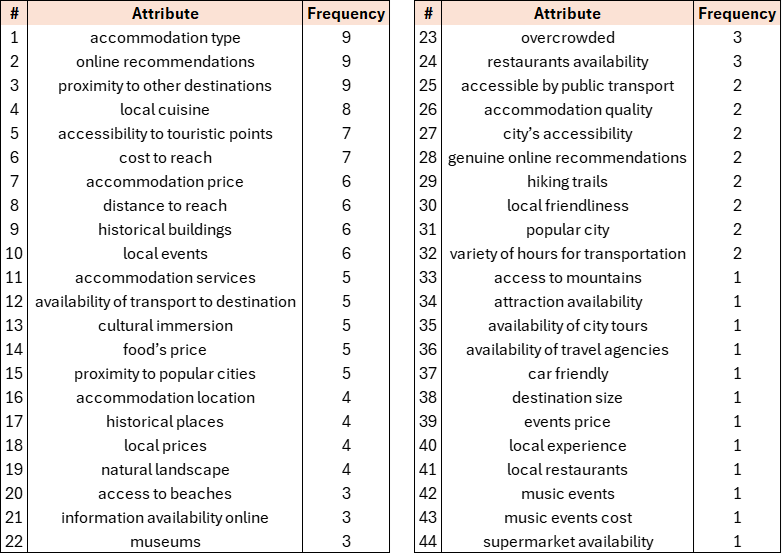
\includegraphics[width=0.9\textwidth]{Images/Qualitative Interviews/attributes_freq.png}
    \captionsetup{font=footnotesize}
    \caption{\textit{Preliminary attributes with their frequency. Source: Author’s own elaboration.}}
    \label{fig:attributesfreq}
\end{figure}


\appendixsection[sec:chatgpt_att]{ChatGPT Attributes}

\begin{figure}[H]
    \centering
    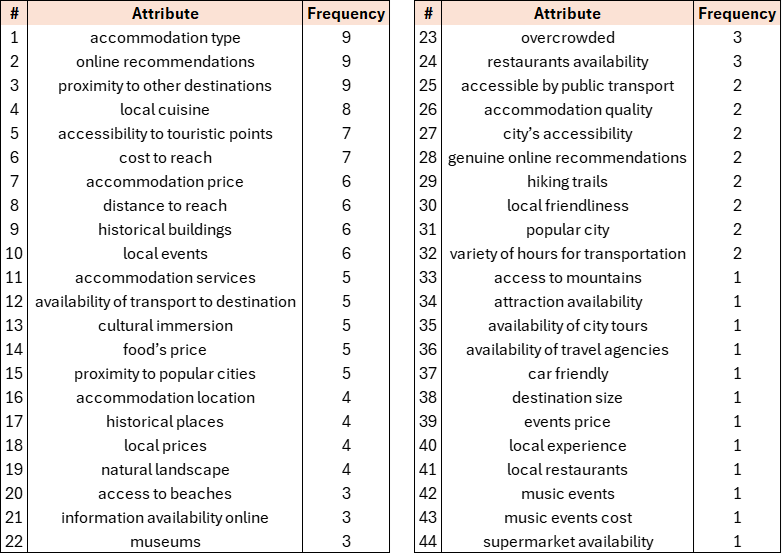
\includegraphics[width=0.9\textwidth]{Images/Qualitative Interviews/attributes_freq.png}
    \captionsetup{font=footnotesize}
    \caption{\textit{Attributes Suggested by ChatGPT. Source: ChatGPT.}}
    \label{fig:chatgpt_I}
\end{figure}

\newpage

\appendixsection[sec:airbnbwords]{Airbnb Top Words}

\begin{figure}[ht]
    \centering
    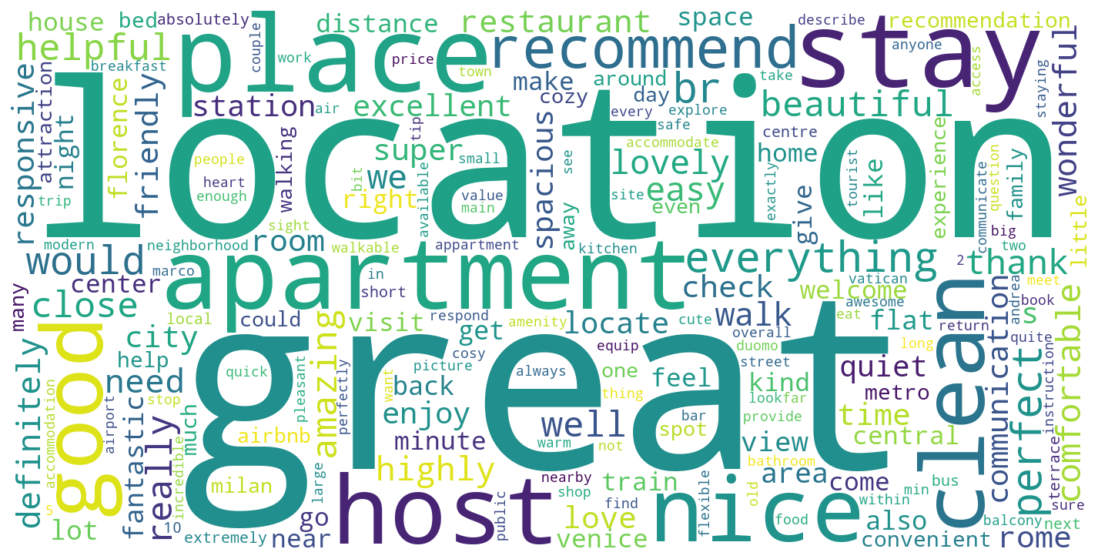
\includegraphics[width=0.7\textwidth]{Analysis/Airbnb Top Words.png}
    \captionsetup{font=footnotesize}
    \caption{\textit{Airbnb Reviews' Top Words. Source: Author’s own elaboration based on Inside Airbnb.}}
    \label{fig:airbnbunigram}
\end{figure}


\appendixsection[sec:bookingtopwords]{Booking.com Top Words}

\begin{figure}[ht]
    \centering
    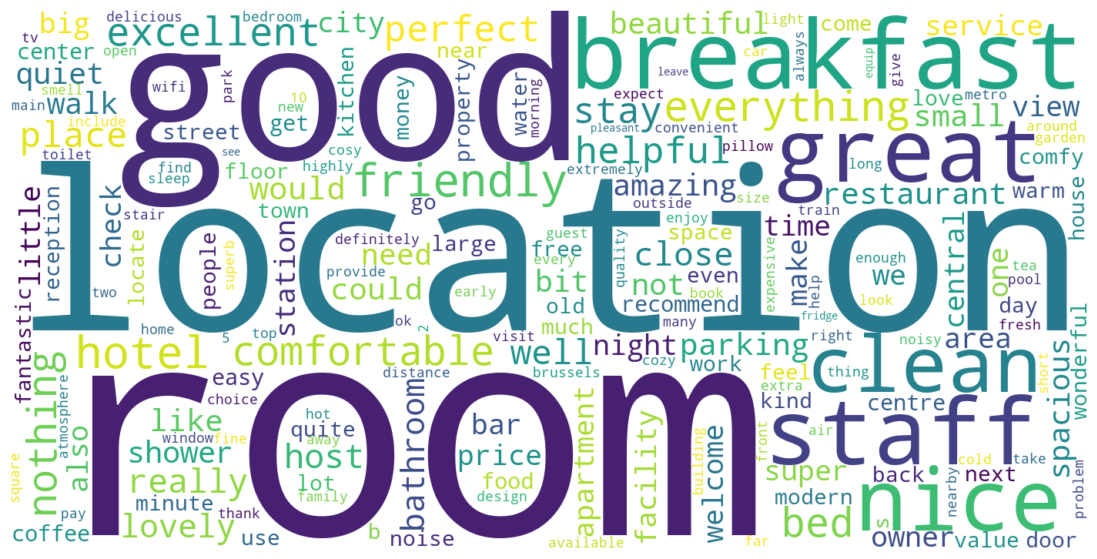
\includegraphics[width=0.7\textwidth]{Analysis/Booking Positive Scores Top Words.png}
    \captionsetup{font=footnotesize}
    \caption{\textit{Booking.com Positive Reviews' Top Words. Source: Author’s own elaboration based on a Kaggle's dataset}}
    \label{fig:bookingpword}
\end{figure}

\begin{figure}[H]
    \centering
    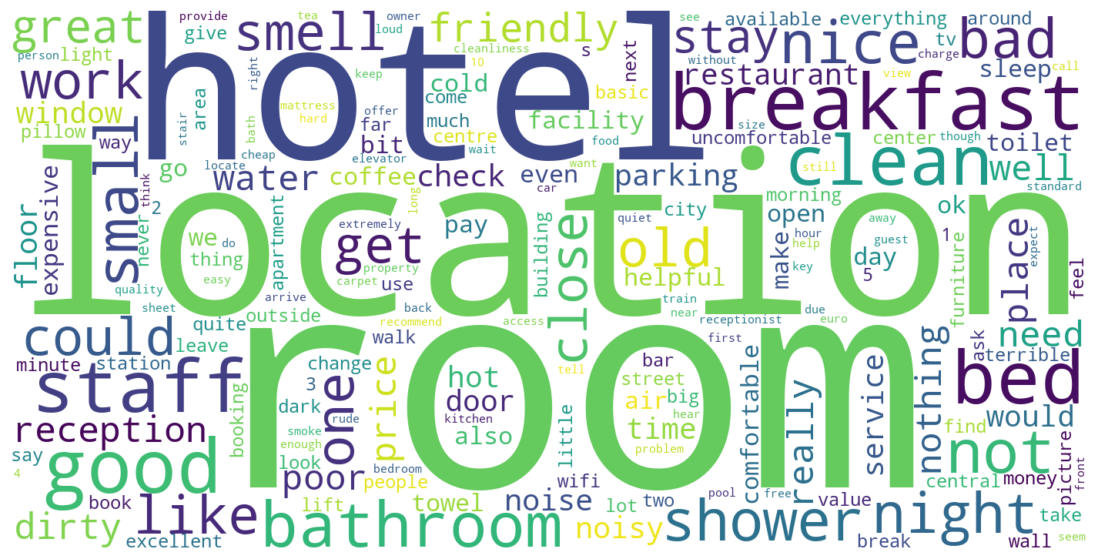
\includegraphics[width=0.7\textwidth]{Analysis/Booking Negative Scores Top Words.png}
    \captionsetup{font=footnotesize}
    \caption{\textit{Booking.com Negative Reviews' Top Words. Source: Author’s own elaboration based on a Kaggle's dataset}}
    \label{fig:bookingnword}
\end{figure}



\includepdf[
  pages=1,
  pagecommand={\appendixsection[sec:explanatorysurvey]{Explanatory Survey}}
]{Material/2. Interviews & Surveys/2. Explanatory Survey/Explanatory Survey (for thesis).pdf}

\includepdf[
  pages=2-,
  pagecommand={}
]{Material/2. Interviews & Surveys/2. Explanatory Survey/Explanatory Survey (for thesis).pdf}

\appendixsection[sec:vwcode]{Pseudocodes for Van Westendorp Model}

\begin{algorithm}[ht]
\caption{Van Westendorp}\label{alg:vw_code}
\begin{algorithmic}[1]
\Require Two curves defined by $(x_1, y_1)$ and $(x_2, y_2)$
\Ensure List of intersection points between the two curves
\State Define common $x$-axis grid $common\_x \gets$ linearly spaced values between the overlapping range of $x_1$ and $x_2$ (500 points)
\State Interpolate $y_1$ and $y_2$ on $common\_x$ using linear interpolation
\State Compute difference $diff \gets y_1^{interp} - y_2^{interp}$
\State Identify sign changes in $diff$ to detect zero-crossings $\rightarrow sign\_change$
\State Initialize empty list $intersections \gets [\,]$
\For{each index $i$ in $sign\_change$}
    \State Estimate $x_{intersect}$ by interpolating where $diff$ crosses zero
    \State Estimate corresponding $y_{intersect}$ from $y_1$
    \State Append $(x_{intersect}, y_{intersect})$ to $intersections$
\EndFor
\State \Return $intersections$
\end{algorithmic}
\end{algorithm}

\newpage
\begin{algorithm}[H]
\caption{Van Westendorp Analysis}\label{alg:van_westendorp_analysis}
\begin{algorithmic}[1]
\Require Data frame $df$ with columns \texttt{too\_cheap}, \texttt{cheap}, \texttt{expensive}, and \texttt{too\_expensive}
\Ensure Intersection points for Van Westendorp price analysis and plotted sensitivity curves

\Function{calculate\_cumulative\_percent}{$series$, $invert$}
    \State Sort values in $series$
    \State Compute cumulative percentages from 1 to 100
    \If{$invert = \text{True}$}
        \State Invert cumulative percentage: $100 - cum\_percent$
    \EndIf
    \State \Return sorted values and cumulative percentages
\EndFunction

\State Compute cumulative percentages for each price perception:
\Statex \hspace{1em} $too\_cheap$, $cheap$, $expensive$, $too\_expensive$

\Comment{--- Compute intersection points ---}
\State $marginal\_cheapness \gets$ \Call{find\_intersection}{$too\_cheap$, $expensive$}
\State $marginal\_expensiveness \gets$ \Call{find\_intersection}{$too\_expensive$, $cheap$}
\State $indifference\_price\_point \gets$ \Call{find\_intersection}{$cheap$, $expensive$}
\State $optimal\_price\_point \gets$ \Call{find\_intersection}{$too\_cheap$, $too\_expensive$}

\Comment{--- Extract x-values for range of acceptable prices ---}
\State $x\_{marginal\_cheapness} \gets$ first element of $marginal\_cheapness$ (if exists)
\State $x\_{marginal\_expensiveness} \gets$ first element of $marginal\_expensiveness$ (if exists)

\Comment{--- Plot curves and intersection points ---}
\State Plot cumulative curves for each price perception
\State Mark intersection points with scatter markers and vertical lines
\State Shade region between marginal cheapness and marginal expensiveness to indicate acceptable price range

\Comment{--- Report numerical results ---}
\State Print:
\begin{itemize}
    \item Point of Marginal Cheapness
    \item Point of Marginal Expensiveness
    \item Indifference Price Point
    \item Optimal Price Point
\end{itemize}

\end{algorithmic}
\end{algorithm}

\newpage
\appendixsection[sec:expsurvresults]{Explanatory Survey Results}

\begin{figure}[H]
    \centering
    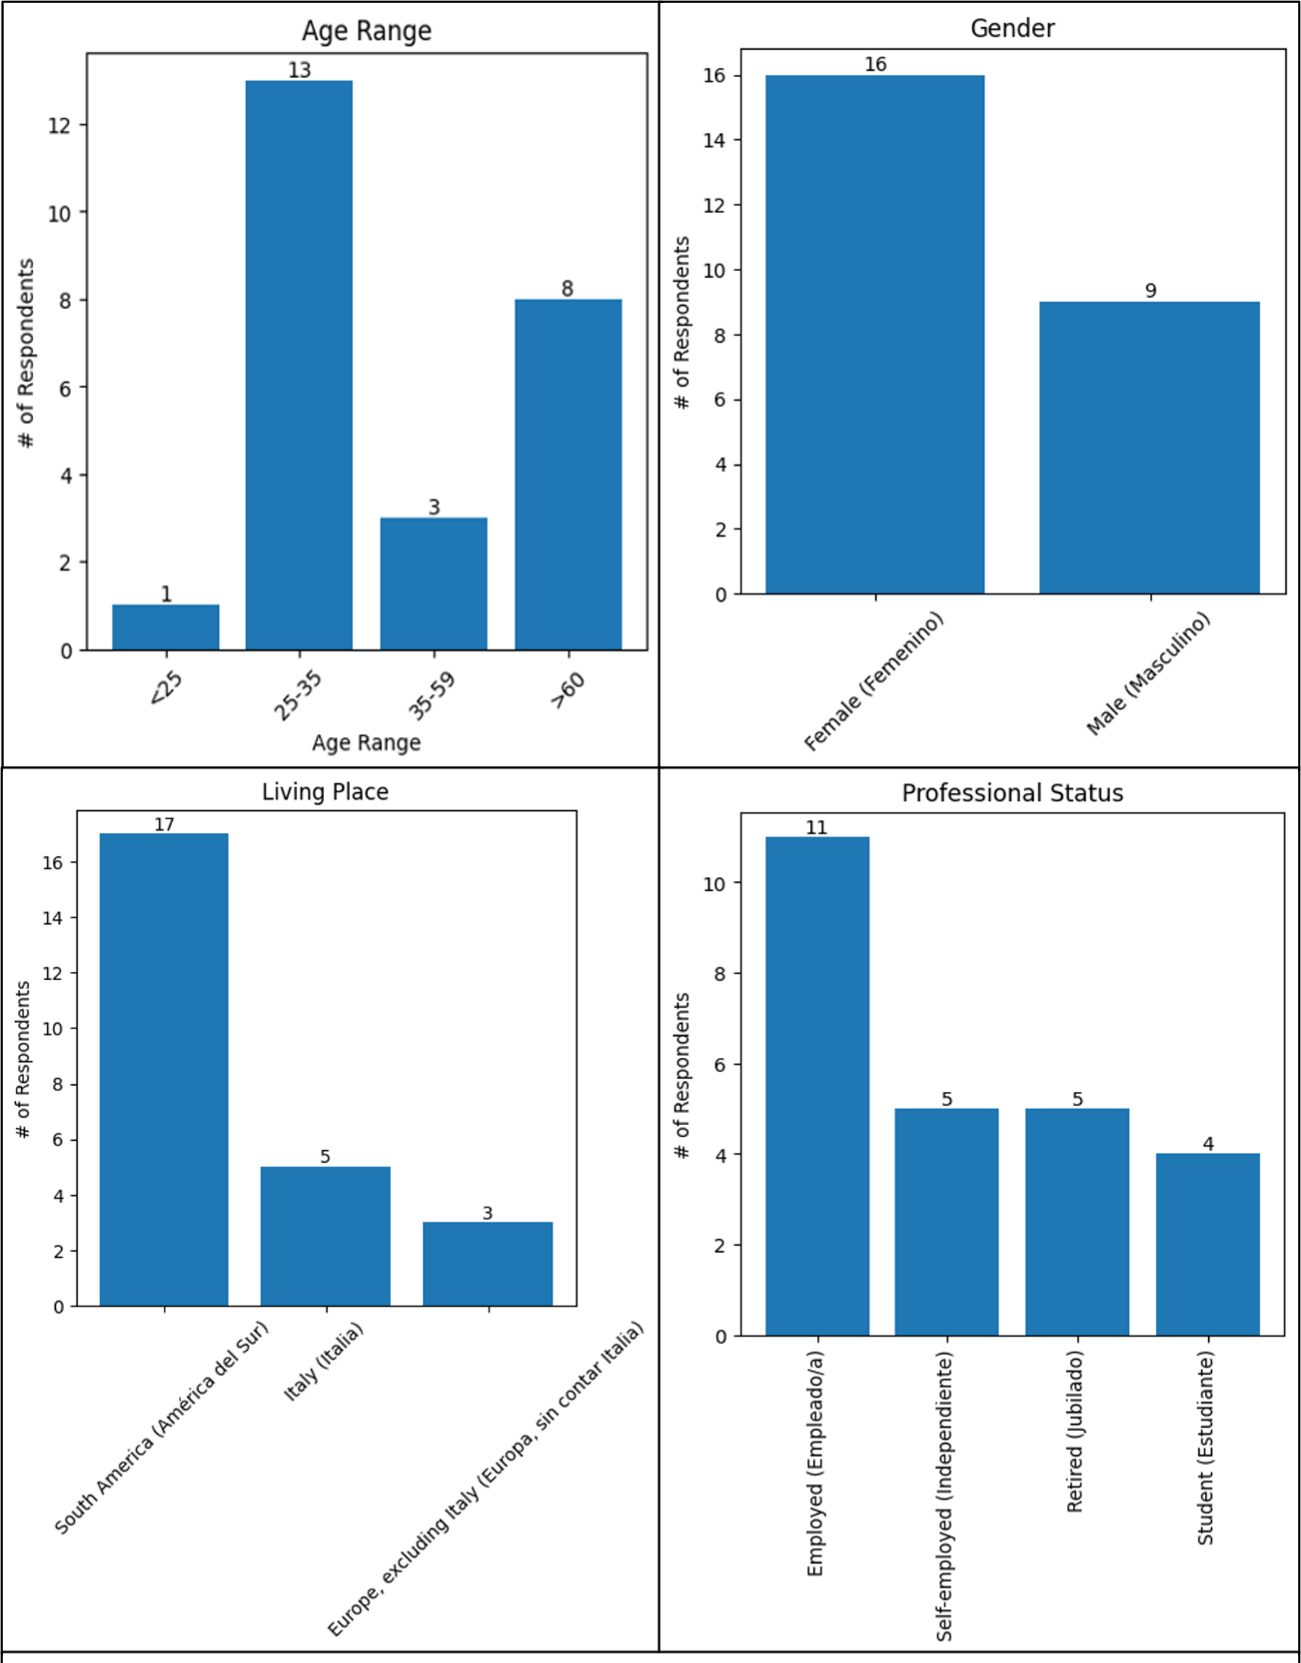
\includegraphics[width=0.9\textwidth]{Images/Explanatory Survey/Descriptive.png}
    \captionsetup{font=footnotesize}
    \caption{\textit{Description of Explanatory Survey's Respondents. Source: Author’s own elaboration.}}
    \label{fig:descriptivedata}
\end{figure}

\newpage
\begin{figure}[H]
    \centering
    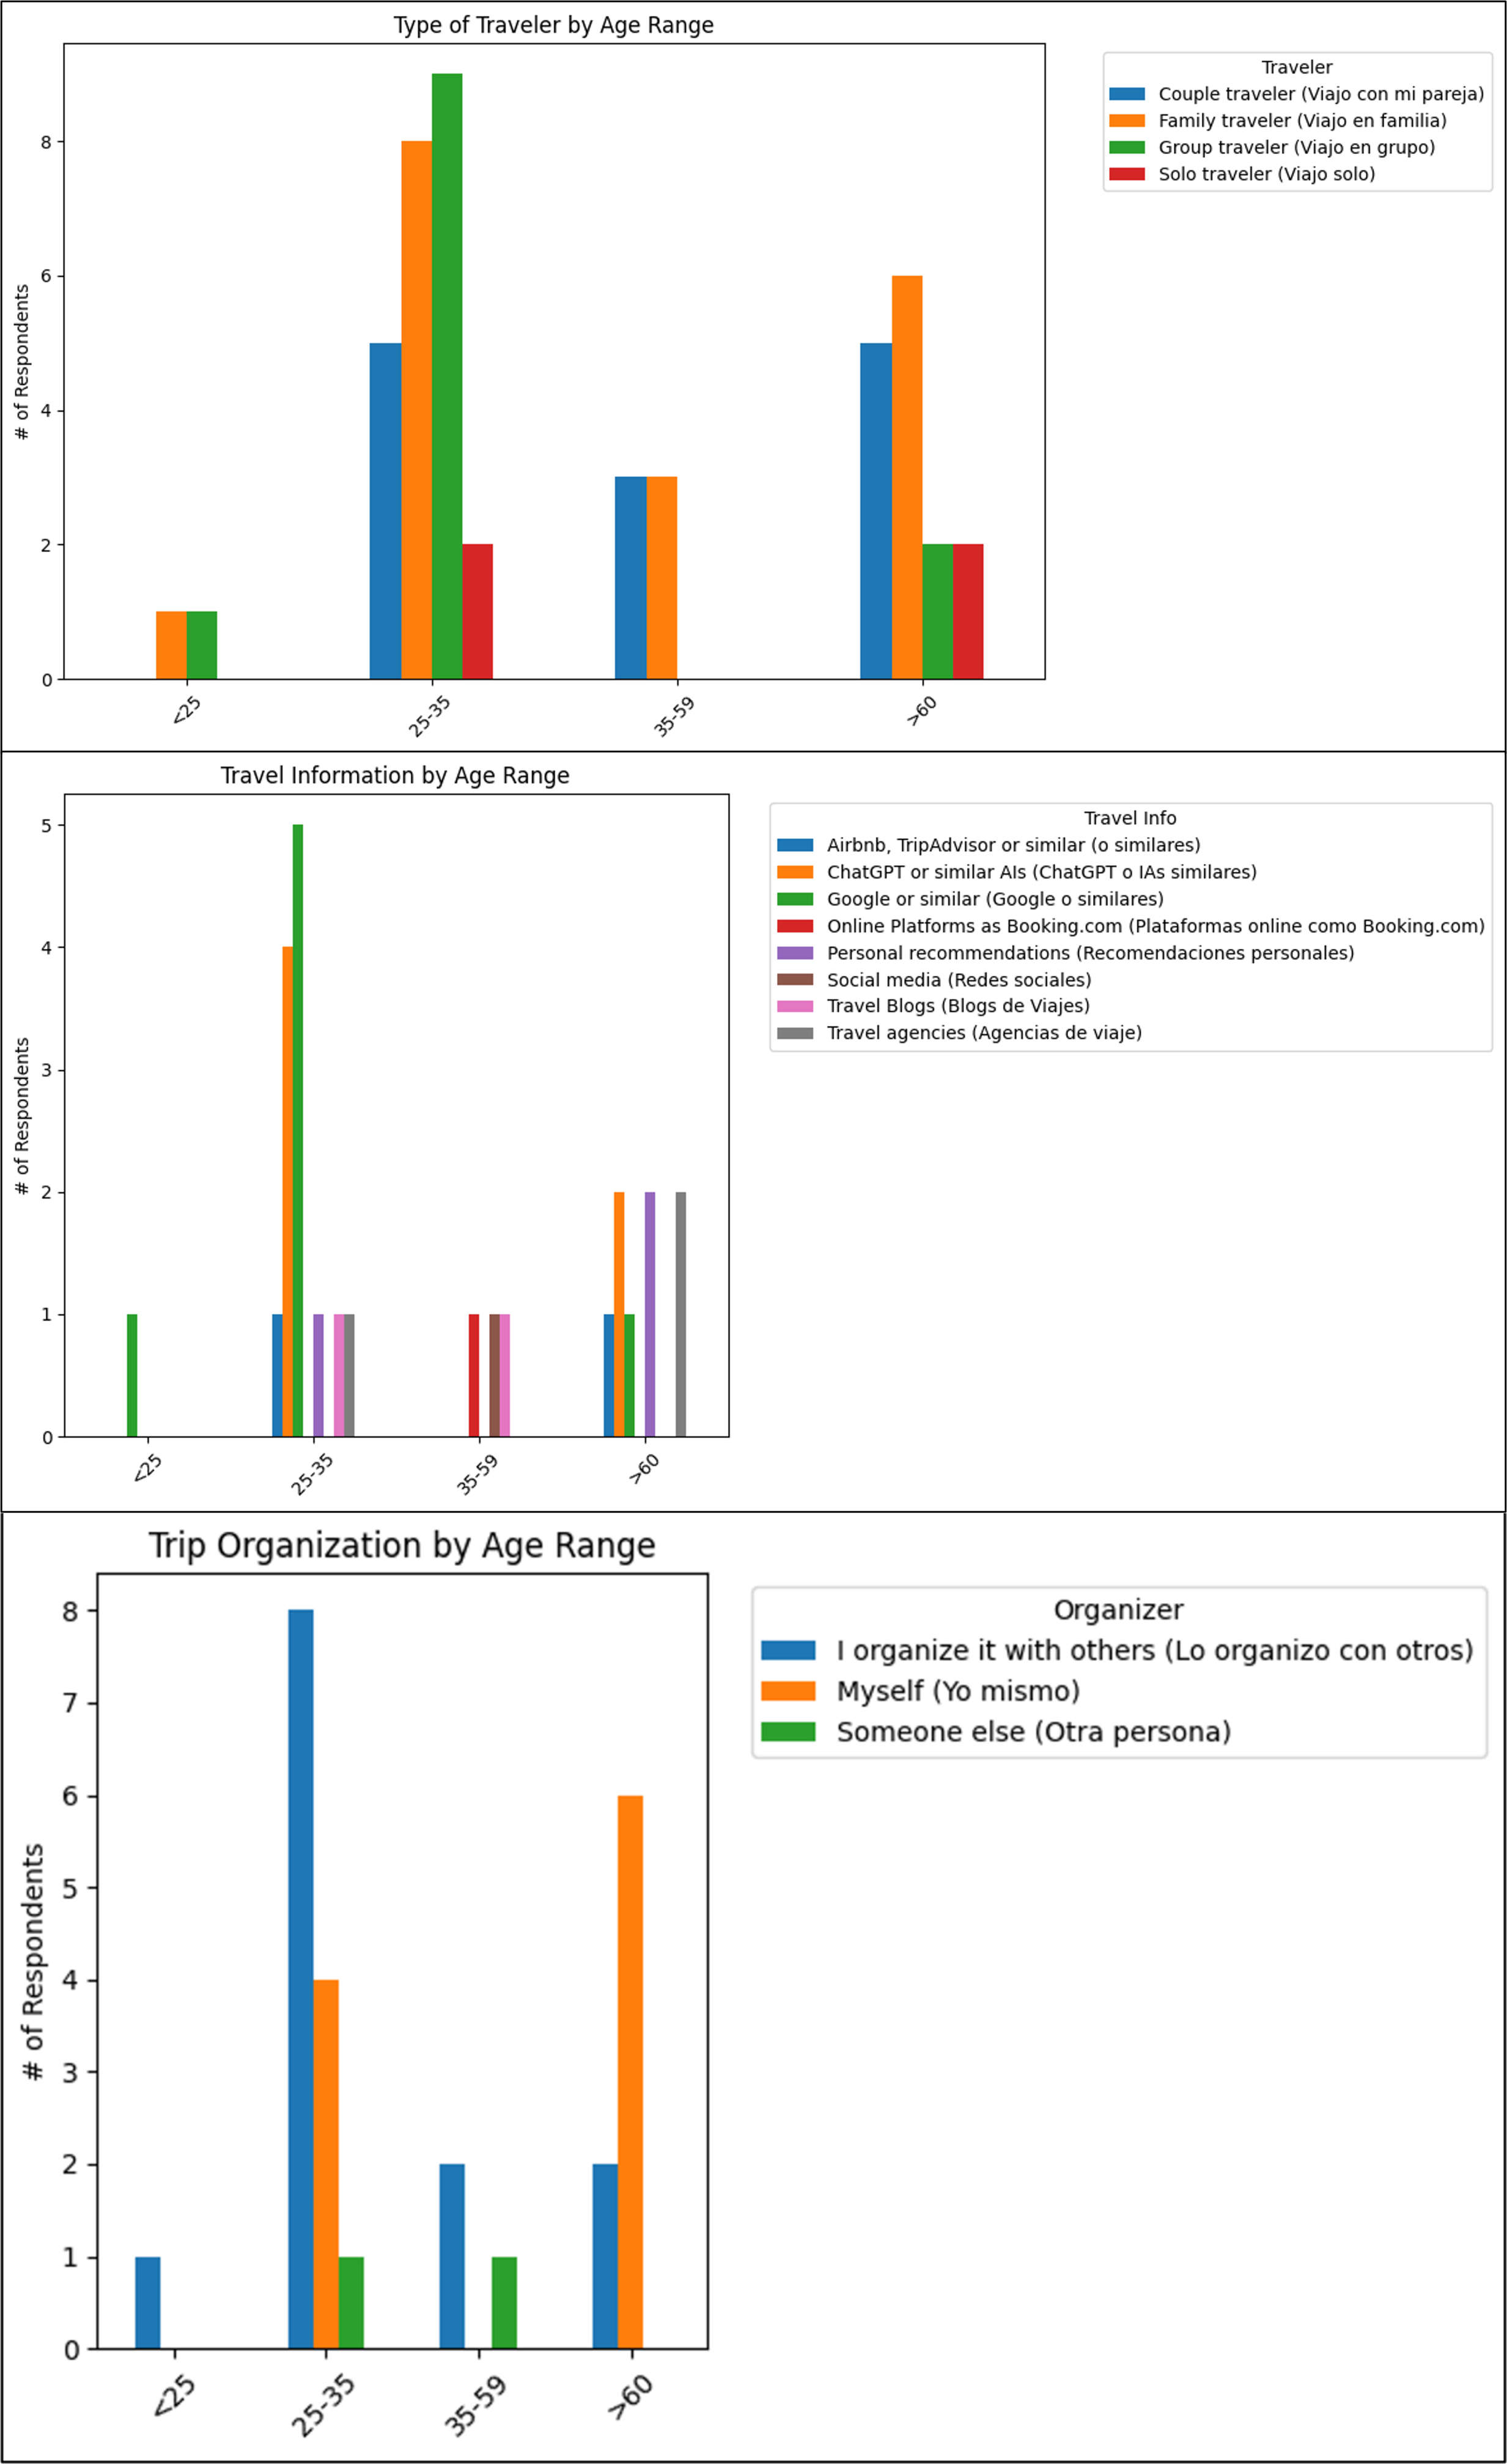
\includegraphics[width=0.9\textwidth]{Images/Explanatory Survey/Descriptive2.png}
    \captionsetup{font=footnotesize}
    \caption{\textit{Description of Explanatory Survey's Respondents. Source: Author’s own elaboration.}}
    \label{fig:descriptivedata2}
\end{figure}


\appendixsection[sec:vanwestendorp]{Van Westendorp Results by Age Group}

\begin{figure}[H]
    \centering
    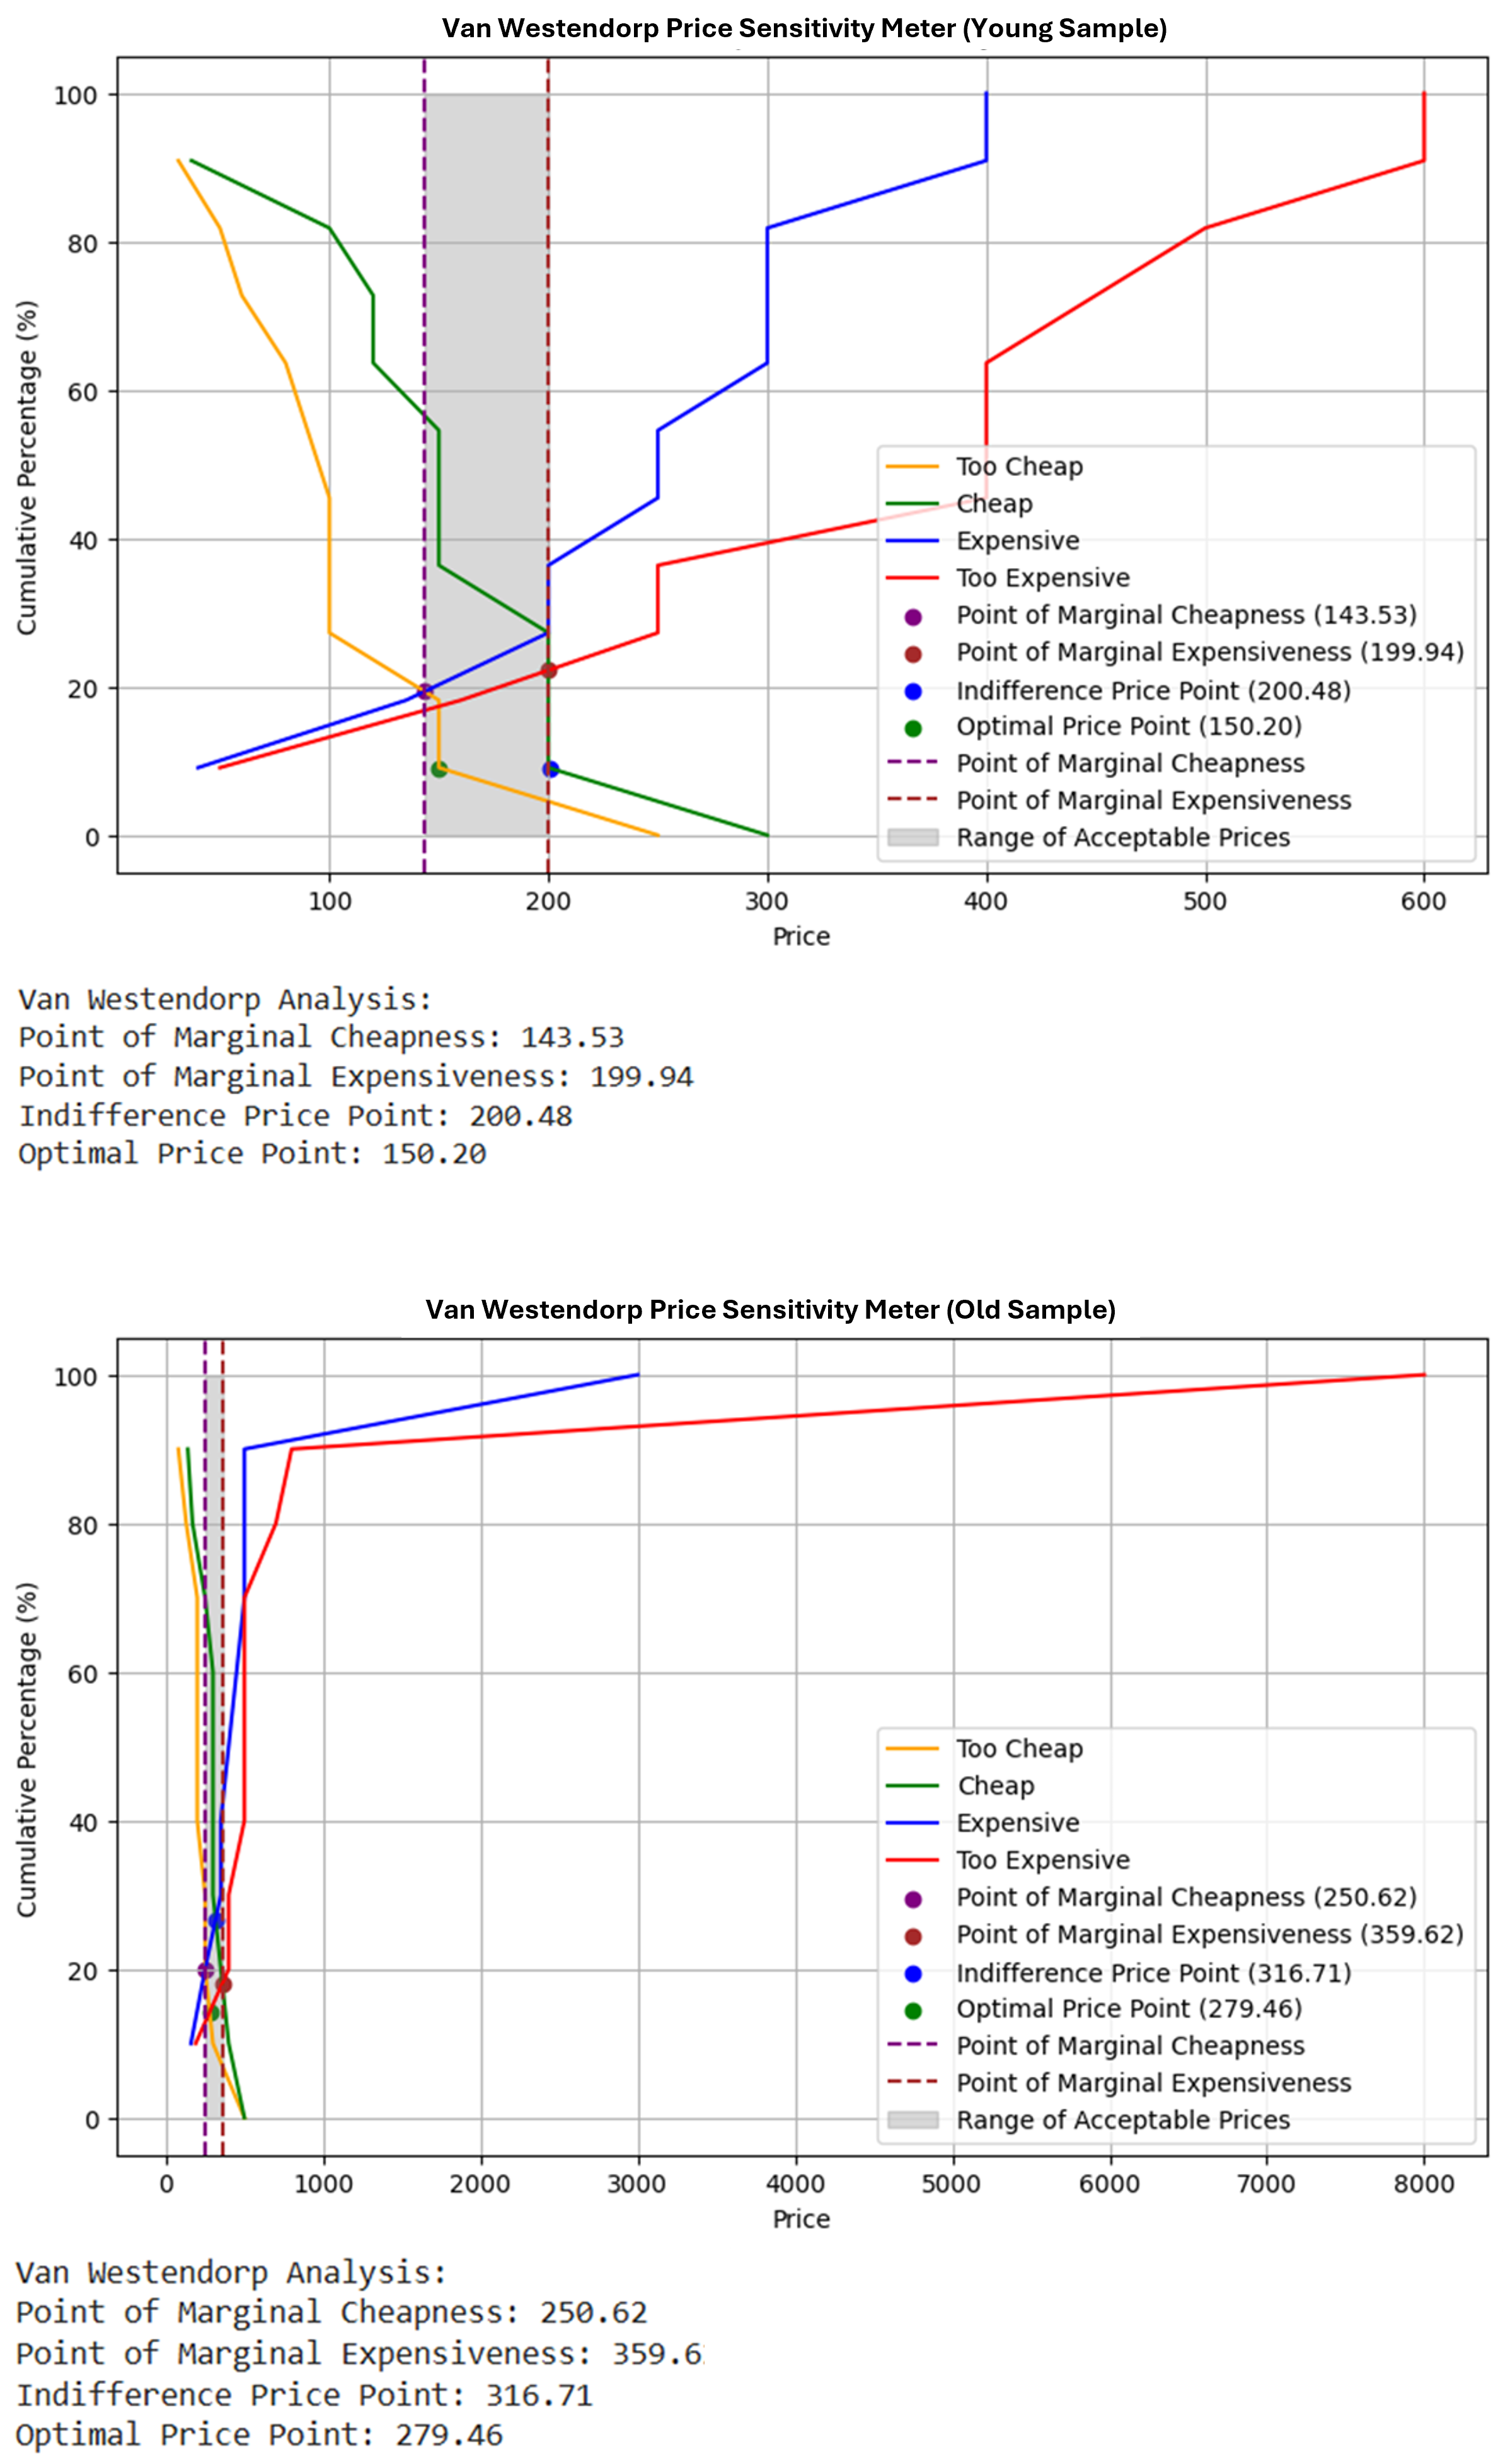
\includegraphics[width=0.7\textwidth]{Images/Explanatory Survey/Van Westendorp (Young & Old).png}
    \captionsetup{font=footnotesize}
    \captionof{figure}{\textit{Van Westendorp Pricing Method by Age Group. Source: Author’s own elaboration.}}
    \label{fig:vwage}
\end{figure}

\includepdf[
  pages=1,
  pagecommand={\appendixsection[sec:quantitativesurvey]{Quantitative Survey}}
]{Material/2. Interviews & Surveys/3. Quantitative Survey/Final Survey_VF.pdf}

\includepdf[
  pages=2-,
  pagecommand={}
]{Material/2. Interviews & Surveys/3. Quantitative Survey/Final Survey_VF.pdf}


\appendixsection[sec:elbowcode]{Pseudocode for Elbow Method}

\begin{algorithm}[H]
\caption{Elbow Method with Gower + KMedoids}\label{alg:elbow}
\begin{algorithmic}[1]
\Require Dataset $X$, range of clusters $k \in [2, 10]$
\State Compute Gower distance matrix: $D \gets gower\_matrix(X)$
\Function{total\_within\_cluster\_distance}{$D, labels$}
    \State $total \gets 0$
    \For{each cluster $c$ in unique($labels$)}
        \State $idx \gets$ indices of points in $c$
        \If{$|idx| > 1$}
            \State $dist \gets D[idx, idx]$
            \State $total \gets total + \frac{\text{sum}(dist)}{2 \times |idx|}$
        \EndIf
    \EndFor
    \State \Return $total$
\EndFunction
\For{each $k$ in $[2, 10]$}
    \State Fit K-Medoids using $D$
    \State Compute within-cluster distance: $score_k \gets$ total\_within\_cluster\_distance($D$, labels)
    \State Append $score_k$ to list
\EndFor
\State Plot $k$ vs. average within-cluster distance
\Ensure Optimal $k$ estimated from the Elbow curve
\end{algorithmic}
\end{algorithm}


\appendixsection[sec:silhouettescore]{Pseudocode for Silhouette Score}

\begin{algorithm}[H]
\caption{Silhouette score Gower KMedoids}\label{alg:silhouette}
\begin{algorithmic}[1]
\Require Distance matrix $D$, range of clusters $k \in [2, 10]$
\For{each $k$ in range}
    \State Fit K-Medoids using $D$
    \State $labels \gets$ model cluster assignments
    \State Compute Silhouette score: $sil_k \gets silhouette(D, labels)$
    \State Append $sil_k$ to list
\EndFor
\State Plot $k$ vs. $silhouette\_score$
\Ensure Optimal $k$ maximizes Silhouette score
\end{algorithmic}
\end{algorithm}

\appendixsection[sec:dbicode]{Pseudocode for Davies Bouldin Index}

\begin{algorithm}[H]
\caption{Davies Bouldin Index with Gower + KMedoids}\label{alg:dbi}
\begin{algorithmic}[1]
\Require Distance matrix $D$, range of clusters $k \in [2, 10]$
\Function{DBI}{$D, labels$}
    \State Identify clusters and compute medoids
    \For{each cluster $i$}
        \State Compute internal dispersion $S_i$
    \EndFor
    \For{each pair $(i,j)$ of clusters}
        \State Compute $M_{ij} \gets \frac{S_i + S_j}{D_{medoid_i, medoid_j}}$
    \EndFor
    \State \Return mean of maximum $M_{ij}$ across clusters
\EndFunction
\For{each $k$ in range}
    \State Fit K-Medoids using $D$
    \State $DBI_k \gets DBI(D, labels)$
    \State Append $DBI_k$ to list
\EndFor
\State Output DBI for each $k$
\Ensure Optimal $k$ minimizes the DBI value
\end{algorithmic}
\end{algorithm}


\appendixsection[sec:pca_clustering]{Biplot with First 2 Components}

\begin{figure}[H]
    \centering
    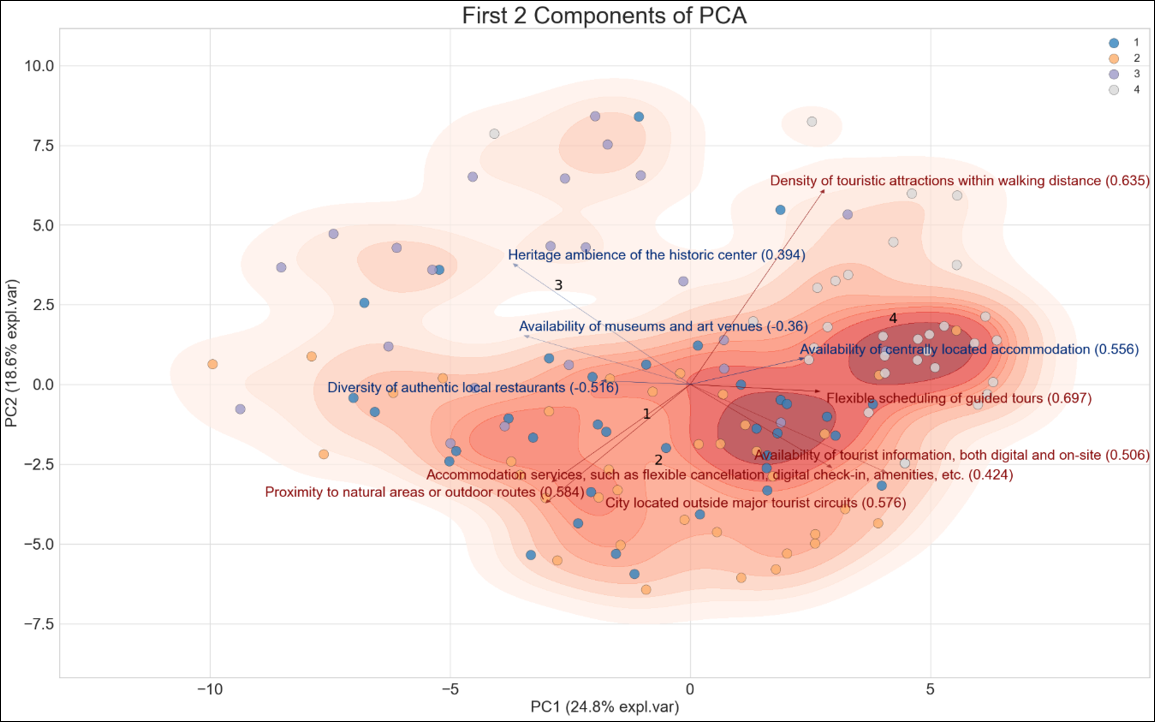
\includegraphics[width=0.9\textwidth]{Images/Quantitative Survey/pca_clusters.png}
    \captionsetup{font=footnotesize}
    \caption{\textit{Biplot with First 2 Components. Source: Author’s own elaboration.}}
    \label{fig:pca_clusters}
\end{figure}



\end{document}